%
%  Top-Level File for PhD Thesis
%  Ryan Kelly
%


\documentclass[a4paper,british,twoside,12pt]{book}

\usepackage{graphics}
\usepackage{graphicx}
\usepackage{subfigure}
\usepackage{amsmath}
\usepackage{amssymb}
\usepackage{amsthm}
\usepackage{verbatim}
\usepackage{algorithm}
\usepackage{algorithmic}
\usepackage{color}
\usepackage{tikz}
\usepackage{bibentry}
\usepackage[numbers]{natbib}
\usepackage{setspace}
\usepackage{fancyhdr}

\definecolor{black}{rgb}{0,0,0}
\definecolor{lightgrey}{rgb}{0.80,0.80,0.80}

% Page margins etc
\topmargin	-13mm
\headheight     6mm
\oddsidemargin  12mm       %left margin of odd page =28mm +oddsidemargin
\evensidemargin 1mm        %left margin of even page =29mm +evensidemargin
\textheight     245mm      
\textwidth      145mm      %width of text across the page =textwidth -5mm

% Page headers and footers for fancy-style pages
\fancyhf{}
\fancyhead[RO]{\sffamily\bfseries \rightmark}
\fancyhead[LE]{\sffamily\bfseries \leftmark}
\fancyfoot[LE]{\setlength{\fboxsep}{2mm}
     \fcolorbox{black}{lightgrey}{\rule{0mm}{4mm}\bfseries \thepage}}
\fancyfoot[RO]{\setlength{\fboxsep}{2mm}
     \fcolorbox{black}{lightgrey}{\rule{0mm}{4mm}\bfseries \thepage}}
\renewcommand{\headrulewidth}{0.3mm}
\renewcommand{\footrulewidth}{0.3mm}
\renewcommand{\footruleskip}{0mm}
\pagestyle{fancy}                   

% matching footers for plain-style pages
\fancypagestyle{plain}{
\fancyhf{}
\fancyfoot[LE]{\setlength{\fboxsep}{2mm}
     \fcolorbox{black}{lightgrey}{\rule{0mm}{4mm}\bfseries \thepage}}
\fancyfoot[RO]{\setlength{\fboxsep}{2mm}
     \fcolorbox{black}{lightgrey}{\rule{0mm}{4mm}\bfseries \thepage}}
\renewcommand{\headrulewidth}{0mm}
\renewcommand{\footrulewidth}{0.3mm}
\renewcommand{\footruleskip}{0mm}
}

% ensure blank pages are completely blank
\makeatletter
\def\cleardoublepage{\clearpage\if@twoside \ifodd\c@page\else
        \hbox{}
        \vspace*{\fill}
        \thispagestyle{empty}
        \newpage
        \if@twocolumn\hbox{}\newpage\fi\fi\fi}
\makeatother


% Proper naming for bibliography
\renewcommand\bibname{References} 

% Redfine default figure placement to "here" (default is {tbp})
\makeatletter
\def\fps@figure{htbp}
\makeatother

% Environment Definitions
\newenvironment{proofsketch}{\begin{proof}[Proof Sketch]}{\end{proof}}
\newtheorem{thm}{Theorem}
\newtheorem{lemma}{Lemma}
\newtheorem{prop}{Proposition}
\newtheorem{example}{Example}
\newtheorem{defn}{Definition}
\newtheorem{defnL}[defn]{Definition}
\newtheoremstyle{thmext}{\topsep}{\topsep}{\itshape}{}{\bfseries}{.}{ }{\thmname{#1}\thmnote{ #3}}
\theoremstyle{thmext}
\newtheorem*{thmext}{Theorem}
\theoremstyle{plain}
\theoremstyle{thmext}
\newtheorem*{lemmaext}{Lemma}
\theoremstyle{plain}

% Pinched from LyX
\newcommand{\noun}[1]{\textsc{#1}}

% Enable fancy chapter headings
\usepackage[Lenny]{fncychap}



\begin{document}

\newcommand{\isdef}{\stackrel{\mbox{\tiny def}}{=}}
\newcommand{\Dt}{\mathcal{D}}
\newcommand{\Reg}{\mathcal{R}}
\newcommand{\Pst}{\mathcal{P}}
\newcommand{\Trn}{\mathcal{T}}
\newcommand{\Kln}{\mathcal{K}}
\newcommand{\TrnA}{\Trn_{a}}
\newcommand{\EKnows}{\mathbf{EKnows}}
\newcommand{\Knows}{\mathbf{Knows}}
\newcommand{\CKnows}{\mathbf{CKnows}}
\newcommand{\KnowsZ}{\mathbf{Knows_{0}}}
\newcommand{\PKnowsZ}{\mathbf{PKnows_{0}}}
\newcommand{\PKnows}{\mathbf{PKnows}}
\newcommand{\KTrans}{\mathbf{KDo}}
\newcommand{\KDo}{\mathbf{KDo}}
\newcommand{\EDo}{\mathbf{EDo}}
\newcommand{\vars}[1]{\bar{#1}}
\newcommand{\PbU}{PbU}
\newcommand{\LNTP}{\mathbf{LNTP}}
\newcommand{\PNA}{\mathbf{PNA}}
\newcommand{\Do}{\mathbf{Do}}
\newcommand{\PstD}{\Pst_{\Dt}}
\newcommand{\PstDI}{\Pst^{1}_{\Dt}}


\begin{titlepage}
\begin{center}
\ \\
\vspace{2cm}
{\bf\LARGE  ASYNCHRONOUS }\\ \vspace{0.5cm}
{\bf\LARGE  MULTI-AGENT REASONING }\\ \vspace{0.5cm}
{\bf\LARGE  IN THE SITUATION CALCULUS } \\
\vspace{3cm}
{\LARGE      Ryan Francis Kelly       }\\
\vspace{5cm}
{\em\large Submitted in total fulfilment of the requirements}\\ \vspace{0.1cm}
{\em\large        of the degree of Doctor of Philosophy     }\\
\vspace{0.5cm}
{\Large             October 2008        }\\
\vspace{2.5cm}
{\bf\large Department of Computer Science\\ and Software Engineering}\\ \vspace{0.5cm}
{\bf\Large        The University of Melbourne     }\\
\vspace{0.5cm}
\end{center}
\end{titlepage}

%Roman numeral numbering for initial section of thesis
\cleardoublepage
\pagenumbering{roman}


\chapter*{Abstract}

This thesis develops several powerful extensions to the situation calculus,
enabling it to reasoning about and planning for teams of agents in rich 
multi-agent domains.  Driven by the desire to cooperative plan and perform
the execution of shared program, we add support for: hidden actions, common knowledge, joint executions.




\chapter*{Declaration}
This is to certify that:
\begin{itemize}
\item[(i)] the thesis comprises only my original work towards the PhD except where indicated in the Preface,
\item[(ii)] due acknowledgement has been made in the text to all other material used,
\item[(iii)] the thesis is less than 100,000 words in length, exclusive of tables, maps, bibliographies, and appendices.
\end{itemize}
\vspace{3cm}
\rule{70mm}{0.1mm}\\
\emph{Ryan Francis Kelly}

\chapter*{Preface}
During the course of this research, a number of public presentations have been
 made which are based on the work presented in this thesis. They are listed
 here for reference.

\nobibliography*
\begin{itemize}
\item \bibentry{kelly06hlp_dps}
\item \bibentry{kelly07sc_persistence}
\item \bibentry{kelly07sc_know_obs}
\item \bibentry{kelly08complex_epistemic_modalities}
\end{itemize}


\chapter*{Acknowledgements} 

First, my heartfelt thanks to my supervisor, Adrian Pearce, for his support
and guidance throughout this research: for constantly reminding me to remember
the bigger picture; for encouraging me to explore any number of wild tangents; 
and for asking the deep questions about how they all fit back together.
Thank you also for trusting me to work in my own time, in my own way, and for
always remaining confident that we would get there in the end.

To my advisory committee, Leon and James, thank you for providing the the
clear heads needed to keep the overall story in focus.  It seems like I
entered each of our progress meetings armed with a vague collection of ideas,
 and left each with a cohesive picture of the road ahead.

I must also acknowledge the generous support of TODO in providing the
Australian Postgraduate Award, without which this research would not have
been possible.

To my fellow students and colleagues at the University of Melbourne -- particularly my office-mates Alan, Terrence, Michelle, Arif, and my CSSEPG accomplices Alauddin, Kapil, Archana, Andrea, Macros -- thanks for making the whole postgrad
experience so rewarding.  And to Sebastian, thanks for our many fascinating
conversations and for being my link into the wider sitcalc community.

For my parents Don and Judy, my brother Matt, and my grandparents Val and
George, thank you for your unwavering support -- financial, physical and emotional -- throughout all of my studies.  Despite the constant jokes about me being ready
for retirement by the time I graduate (those \emph{were} just jokes, right??) I
have always known that I could count on your unconditional love and support.

Finally, but of course most importantly, to my wife Lauren: thank you
for your unending love and understanding; for tolerating weeks of procrastination
followed by weeks fervent study; for keeping me firmly grounded in the real
world; and for simply being so excited about the whole 
endeavour.  Thank you.



% Contents and other lists are single-spaced
\singlespace
\cleardoublepage
\tableofcontents
\listoftables
\listoffigures
\listofalgorithms

% One-half line spaces for main body
% Also swicth to arabic page numbers
\cleardoublepage
\onehalfspace
\pagenumbering{arabic}

\chapter{Introduction}
%\minitoc

This thesis develops techniques for the cooperative execution of a shared 
program by a team of agents in rich multi-agent domain.  To make this more 
concrete, let us begin with a short motivating example which will be used 
throughout the thesis:

\begin{quote}
You have just taken possession of a team of robotic chefs.  It is your 
task to program the chefs to prepare a delicious meal.
\end{quote} 



\begin{itemize}
\item motivating example: cooking agents
\item introduce HLP paradigm, briefly argue in its favour
\item major limitation: focused on single-agent systems
\item the "MIndiGolog Vision": cooperative execution of a HLP
\item secondary aim: general-purpose tools for HLP in multi-agent domains
\item achievements in this thesis:
  \begin{itemize}
  \item MIndiGolog: HLP semantics suitable for multi-agent domains
  \item New reasoning technique for univsersally quantified queries
  \item Robustly multi-agent account of knowledge, common knowledge
  \item Semantics and techniques for cooperative planning of a legal execution
  \item Techniques for online execution using "social laws" coordination
  \item Implementations in Oz with distributed execution planning
  \end{itemize}
\end{itemize}




\chapter{Background}

\label{ch:background}

This chapter covers general background material for the thesis, and
serves as a brief literature review. More specific background material
may be found at the beginning of each subsequent chapter.

We begin by introducing the base language of the situation calculus
in section \ref{sec:Background:The-Situation-Calculus}, along with
the {}``cooking agents'' example domain which will be used throughout
the thesis. Section \ref{sec:Background:Golog} introduces the Golog
family of programming languages, which are the standard formalism
for representing complex tasks in the situation calculus. Reasoning
about knowledge is covered in section \ref{sec:Background:Epistemic-Reasoning}.
Finally, section \ref{sec:Background:Mozart/Oz} introduces the Mozart
programming system, which forms the basis of our implementation. Basic
familiarity with with formal logic (including first-order, second-order,
and modal logic) is assumed throughout; readers requiring background
on such material may find a gentle introduction in \citep{kelly96logic}
and a more detailed treatment in \citep{fitting96fol_book,blakcburn02modal_logic}.

While there are no new results presented in this chapter, it does
introduce some novel notation which will be needed later in the thesis.
It is introduced here to maintain consistency of the presentation.


\section{The Situation Calculus\label{sec:Background:The-Situation-Calculus}}

The situation calculus is a formalism for describing and reasoning
about dynamic worlds. It was first introduced by \citet{McCHay69sitcalc}
and has since been significantly expanded and formalised \citep{reiter91frameprob,pirri99contributions_sitcalc}.
We use the particular variant due to Reiter et. al. at the University
of Toronto, sometimes called the {}``Toronto school'' or {}``situations-as-histories''
version \citep{levesque98sc_foundations,pirri99contributions_sitcalc}.

A brief overview is presented below. Readers familiar with the situation
calculus should note our generalised characterisation of the background
theory $\Dt_{bg}$, our generalisation of the $Poss$ fluent to action
description predicates, and the parameterised {}``future situation''
predicate $s<_{\alpha}s'$.


\subsection{Notation\label{sec:Background:SC:Notation}}

The language $\mathcal{L}_{sitcalc}$ of the situation calculus is
a many-sorted language of first-order logic with equality, augmented
with a second-order induction axiom, containing the following disjoint
sorts:

\begin{itemize}
\item \emph{\noun{Action}} terms are functions denoting individual instantaneous
events that can cause the state of the world to change; 
\item \noun{Situation} terms are histories of the actions that have occurred
in the world, with the initial situation represented by $S_{0}$ and
successive situations built using the function $do\,:\, Action\times Situation\rightarrow Situation$; 
\item \noun{Object} terms represent any other object in the domain. 
\end{itemize}
\emph{Fluents} are predicates or functions that represent properties
of the world that may change between situations, and so take a situation
term as their final argument. Predicates and functions that do not
take a situation term are called \emph{rigid}. No functions other
than $S_{0}$ and $do$ take values of sort \noun{Situation.}

$\mathcal{L}_{sitcalc}$ contains the standard alphabet of logical
connectives, countably infinitely many variables of each sort, countably
infinitely many predicates of each arity, etc; for a complete definition,
consult the foundational paper by \citet{pirri99contributions_sitcalc}.
We follow standard naming conventions for the situation calculus:
upper-case roman names indicate constants; lower-case roman names
indicate variables; greek names indicate meta-variables or formula
templates. All axioms universally close over their free variables
at outermost scope. The notation $\vars{t}$ indicates a vector of
terms of context-appropriate arity and type. The connectives $\wedge$,
$\neg$, $\exists$ are taken as primitive, with $\vee$, $\rightarrow$,
$\equiv$, $\forall$ defined in the usual manner.

In multi-agent domains it is customary to introduce the sort \noun{Agent
}as a sub-sort of \noun{Object} to explicitly represent the agents
operating in the world, and we will do so here. The first argument
of each action term gives the performing agent.

\medskip{}


For concreteness, let us present some formulae from an example domain
that will be used throughout the thesis. In the {}``cooking agents''
domain a group of robotic chefs inhabit a kitchen containing various
ingredients and utensils, and they must cooperate to prepare a meal.
Some example statements from this domain include {}``Ann is not holding
the knife initially'' and {}``Bob is holding the knife after he
picks it up''. Formally:\begin{gather*}
\neg Holding(Ann,Knife1,S_{0})\\
Holding(Bob,Knife1,do(pickup(Bob,Knife1),S_{0}))\end{gather*}


\medskip{}


Complex properties of the state of the world are represented using
\emph{uniform formulae}. These are basically logical combinations
of fluents referring to a common situation term. For the moment we
restrict ourselves to \emph{objective} uniform formulae; the complete
definition includes statements about knowledge and will be introduced
following that material.

\begin{defnL}
[{Uniform~Terms}] Let $s$ be a fixed situation term, $r$
an arbitrary rigid function symbol, $f$ an arbitrary fluent function
symbol, and $x$ a variable that is not of sort \noun{Situation}.
Then the terms uniform in $s$ are the smallest set of syntactically-valid
terms satisfying:\[
\tau\,::=s\,|\, x\,|\, r(\vars{\tau})\,|\, f(\vars{\tau},s)\]

\begin{defnL}
[{Objective~Uniform~Formulae}] Let $s$ be a fixed situation
term, $R$ an arbitrary rigid predicate, $F$ an arbitrary fluent
predicate, $\tau$ an arbitrary of term uniform in $s$, and $x$
an arbitrary variable that is not of sort \noun{Situation}. Then the
objective formulae uniform in $s$ are the smallest set of syntactically-valid
formulae satisfying:\[
\phi::=F(\vars{\tau},s)\,|\, R(\vars{\tau})\,|\,\tau_{1}=\tau_{2}\,|\,\phi_{1}\wedge\phi_{2}\,|\,\neg\phi\,|\,\exists x:\phi\]

\end{defnL}
\end{defnL}
The meta-variable $\phi$ is used throughout to refer to an arbitrary
uniform formula. Since they represent properties of the world, it
is frequently useful to evaluate uniform formulae at several different
situation terms. The notation $\phi[s']$ represents a uniform formula
with the particular situation $s'$ inserted into all its fluents.
We will often suppress the situation term in $\phi$ to simplify the
presentation, using $\phi^{-1}$ to represent a uniform formula with
the situation argument removed from all its fluents. For example,
if $\phi=Holding(Ann,Knife,s)\wedge Holding(Bob,Bowl,s)$, then we
have:\begin{gather*}
\phi[s']\,=\, Holding(Ann,Knife,s')\wedge Holding(Bob,Bowl,s')\\
\phi^{-1}\,=\, Holding(Ann,Knife)\wedge Holding(Bob,Bowl)\end{gather*}


\newpage{}


\subsection{Axioms\label{sec:Background:SC:Axioms}}

The dynamics of a particular domain are captured by a set of sentences
from $\mathcal{L}_{sitcalc}$ called a \emph{basic action theory}.
Queries about the behaviour of the world are posed as logical entailment
queries relative to this theory.

\begin{defnL}
[{Basic~Action~Theory}] A basic action theory, denoted
$\Dt$, is a set of situation calculus sentences (of the specific
syntactic form outlined below) describing a particular dynamic world.
It consists of the following disjoint sets: the foundational axioms
of the situation calculus ($\Sigma$); action description axioms defining
preconditions etc for each action ($\Dt_{ad}$); successor state axioms
describing how primitive fluents change between situations ($\Dt_{ssa}$);
axioms describing the value of primitive fluents in the initial situation
($\Dt_{S_{0}}$); and axioms describing the static background facts
of the domain ($\Dt_{bg}$):\[
\Dt=\Sigma\cup\Dt_{ad}\cup\Dt_{ssa}\cup\Dt_{S_{0}}\cup\Dt_{bg}\]

\end{defnL}
These axioms must satisfy some simple consistency criteria to constitute
a valid domain description \citep{pirri99contributions_sitcalc}.
We assume an arbitrary, but fixed, basic action theory.

\medskip{}


The set $\Dt_{bg}$ characterises the static aspects of the domain,
and contains all axioms defining rigid predicates or functions. It
contains unique names axioms asserting that action terms with different
types or arguments are in fact different, e.g.:\begin{gather*}
pickup(agt,obj)\neq drop(agt,obj)\\
pickup(agt_{1},obj_{1})=pickup(agt_{2},obj_{2})\,\rightarrow\, agt_{1}=agt_{2}\,\wedge\, obj_{1}=obj_{2}\end{gather*}


It also contains domain closure axioms for the sorts \noun{Action,
Agent} and \noun{Object}, and defines the function $actor(a)$ to
give the agent performing an action.

\medskip{}


The set $\Dt_{ssa}$ contains one \emph{successor state axiom} for
each primitive fluent in the domain, providing a monotonic solution
to the frame problem for that fluent. These axioms have the following
general form: \[
F(\vars{x},do(a,s))\equiv\Phi_{F}^{+}(\vars{x},a,s)\,\,\vee\,\, F(\vars{x},s)\wedge\neg\Phi_{F}^{-}(\vars{x},a,s)\]


Here $\Phi_{F}^{+}$ and $\Phi_{F}^{-}$ are formulae uniform in $s$.
This may be read as {}``$F$ is true after performing $a$ if $a$
made it true, or it was previously true and $a$ did not make it false''.
For example, the $Holding$ fluent may be specified using:\begin{multline*}
Holding(agt,obj,do(a,s))\,\equiv\, a=pickup(agt,obj)\\
\vee\, Holding(agt,obj,s)\wedge a\ne drop(agt,obj)\end{multline*}


\medskip{}


The set $\Dt_{ad}$ generalises the standard \emph{action precondition
axioms} \citep{pirri99contributions_sitcalc} to define fluents describing
various aspects of the performance of an action, which we call \emph{action
description predicates}. The predicate $Poss(a,s)$ is the canonical
example, indicating whether it is possible to perform an action in
a given situation. For example, it is only possible for an agent to
pickup an object if nobody is currently holding it:\[
Poss(pickup(agt,obj),s)\equiv\neg\exists agt_{2}:\, Holding(agt_{2},obj,s)\]
 $\Dt_{ad}$ contains one axiom of the form $Poss(A(\vars{x}),s)\equiv\Phi_{Poss}^{A}(\vars{x},s)$
for each type of action $A$. Any number of predicates and functions
can be defined in this way, and we will use the meta-variable $\alpha$
for an arbitrary action description predicate.

We assume that these definitions are finitely enumerable and well-founded,
allowing them to be expanded down to primitive fluents even when they
refer to an action variable. For example, we assume that $Poss(a,s)$
can be replaced by an enumeration over action types such as the following:\[
Poss(a,s)\equiv\,\, a=A_{1}(\vars{x}_{1})\wedge\Phi_{Poss}^{A_{1}}(\vars{x}_{1},s)\,\vee\,\dots\,\vee a=A_{n}(\vars{x}_{n})\wedge\Phi_{Poss}^{A_{n}}(\vars{x}_{n},s)\]


\medskip{}


The foundational axioms $\Sigma$ ensure that situations form a branching-time
account of the world state. There is a distinguished situation $S_{0}$
called the \emph{initial situation}. Situations in general form a
tree structure with the initial situation at the root and $do(a,s)$
constructing the successor situation resulting when the action $a$
is performed in $s$. All situations thus produced are distinct:\[
do(a_{1},s_{1})=do(a_{2},s_{2})\,\rightarrow\, a_{1}=a_{2}\,\wedge\, s_{1}=s_{2}\]


We abbreviate the performance of several successive actions by writing:\[
do([a_{1},\dots,a_{n}],s)\,\isdef\, do(a_{n},do(\dots,do(a_{1},s)))\]


The relation $s\sqsubset s'$ indicates that $s'$ is in the future
of $s$ and is defined as follows:\begin{gather*}
\neg(s\sqsubset S_{0})\\
s\sqsubset do(a,s')\equiv s\sqsubseteq s'\end{gather*}


Here $s\sqsubseteq s'$ is the standard abbreviation for $s\sqsubset s'\vee s=s'$.
There is also a second-order induction axiom asserting that all situations
must be constructed in this way, which is needed to prove statements
that universally quantify over situations:\[
\forall P:\,\left[P(S_{0})\wedge\forall s,a:\,\left(P(s)\rightarrow P(do(a,s))\right)\right]\,\rightarrow\,\forall s:\, P(s)\]


The notation for {}``in the future of'' can be extended to consider
only those futures in which all actions satisfy a particular action
description predicate. We include a relation $<_{\alpha}$ for each
action description predicate $\alpha$, with the following definitions:\begin{gather*}
\neg\left(s<_{\alpha}S_{0}\right)\\
s<_{\alpha}do(a,s')\equiv s\leq_{\alpha}s'\wedge\alpha(a,s')\end{gather*}


The \emph{legal situations} are those in which every action was possible
to perform in the preceding situation. These are of fundamental importance,
as they are the only situations that could be reached in the real
world. The \emph{root} of a situation is the initial situation from
which it was constructed:\begin{gather*}
root(S_{0})=s\\
root(do(c,s))=root(s)\\
Legal(s)\,\equiv\, root(s)\leq_{Poss}s\end{gather*}


\medskip{}


The set $\Dt_{S_{0}}$ describes the actual state of the world before
any actions are performed. It is a collection of sentences of the
form $\phi[S_{0}]$ stating what holds in the initial situation.\medskip{}



\subsection{Reasoning}

One of the attractions of the situation calculus is the existence
of effective reasoning procedures for certain types of query. These
are generally based on syntactic manipulation of a query into a form
that is more amenable to reasoning -- for example, because it can
be proven without using some of the axioms from $\Dt$.


\subsubsection{Types of Reasoning}

TODO: reasoning in the {}``fluent domain''

In the general case, answering a query about a basic action theory
$\Dt$ is a theorem-proving task in second-order logic (denoted SOL)
due to the induction axiom included in the foundational axioms:\[
\Dt\models_{SOL}\psi\]
 This is clearly problematic for effective automated reasoning, but
fortunately there exist particular syntactic forms for which some
of the axioms in $\mathcal{D}$ are not required.

If a query existentially quantifies over situation terms, it can be
answered without the induction axiom (denoted $I$) and thus using
only first-order logic (FOL) \citep{pirri99contributions_sitcalc}:\[
\Dt\models_{SOL}\exists s:\,\psi(s)\,\,\,\,\mathrm{iff}\,\,\,\,\Dt\models_{FOL}\exists s:\,\psi(s)\]


Even simpler are queries uniform in the initial situation, which can
be answered using only first-order logic and a limited set of axioms:\[
\mathcal{D}\models_{SOL}\phi[S_{0}]\,\,\,\,\,\mathit{\mathrm{iff}}\,\,\,\,\,\Dt_{S_{0}}\cup\Dt_{bg}\models_{FOL}\phi[S_{0}]\]


Since the axioms $\Dt_{S_{0}}\cup\Dt_{bg}$ often satisfy the closed-world
assumption, provers such as Prolog can be employed to handle this
type of query quite effectively. Effective reasoning depends on transforming
queries into more easily-handled forms such as this. \\



\subsubsection{Regression}

TODO: more thorough explanation of regression, and relation to other
formulations (e.g. all-at-once regression)\\


The principle tool for effective reasoning in the situation calculus
is the regression meta-operator $\Reg_{\Dt}$ \citep{pirri99contributions_sitcalc},
a syntactic manipulation that can transform a formula uniform in $do(a,s)$
into an equivalent formula that is uniform in $s$:\[
\Dt\,\models\,\phi[do(a,s)]\equiv\Reg_{\Dt}(\phi[do(a,s)])[s]\]


Since $\Dt$ is fixed, we drop the subscript and simply write $\Reg$
for regression. Its operation is defined by a set of \emph{regression
rules} such as those shown below:\begin{align*}
\Reg(\phi_{1}\wedge\phi_{2})\isdef & \,\,\,\Reg(\phi_{1})\wedge\Reg(\phi_{2})\\
\Reg(Poss(a,s))\isdef & \,\,\,\bigvee\exists\vars{x}:\, a=A(\vars{x})\wedge\Reg(\Phi_{Poss}^{A}(\vars{x},s))\\
\Reg(F(\vars{x},do(a,s)))\isdef & \,\,\,\Phi_{F}^{+}(\vars{x},a,s)\,\,\vee\,\, F(\vars{x},s)\wedge\neg\Phi_{F}^{-}(\vars{x},a,s)\end{align*}


Each application of the regression operator replaces action description
predicates with their definitions from $\Dt_{ad}$ and primitive fluents
with their successor state axioms from $\Dt_{ssa}$, {}``unwinding''
a single action from each situation term in the query.

Repeated applications of this operator, denoted by $\Reg^{*}$, can
transform a query about some future situation into a query about the
initial situation only, which is much easier to answer. The axioms
$\Dt_{ad}$ and $\Dt_{ssa}$ are essentially {}``compiled into''
the query. The trade-off is that the length of the regressed query
may be exponential in the length of $\phi$. While an efficiency gain
is not guaranteed, regression has proven a very effective technique
in practice \citep{levesque97golog,pirri99contributions_sitcalc}.

When dealing with situation-suppressed uniform formulae, we will use
a two-argument operator $\Reg(\phi,a)$ to indicate the regression
of $\phi$ over the action $a$. It should be read as a shorthand
for $\Reg(\phi[do(a,s)])^{-1}$ using the situation-suppression operator
from section \ref{sec:Background:SC:Notation}.

One shortcoming of the regression operator is the potential for an
exponential growth in the length of the query \citep{reiter91frameprob}.
While this cannot be completely overcome in general, there are certain
restrictions that can be placed on the domain to ensure it is not
a problem. TODO: find references: context-free SSAs, local-effect
SSAs.


\subsubsection{Decidability}

Even given the use of regression to reduce the number of axioms required,
reasoning still requires first-order logic and is thus only semi-decidable
in general. Practical systems implemented on top of the situation
calculus typically enforce additional restrictions on the domain in
order to gain decidability. For example, implementations in Prolog
typically assume that the axioms about the initial situation satisfy
the closed-world assumption, so initial situation reasoning can be
performed using Prologs more effecient theorem proving instead of
a full first-order prover.

Another option is to assume the \noun{Action} and \noun{Object} domains
are finite, allowing static domain reasoning to be performed using
propositional logic, which is decidable \citep{giacomo99impl_robots,levesque04krr_book}.
Recent work by \citet{yu07twovar_sitcalc} shows how domains can be
restricted to the two-variable fragment of first-order logic, which
is also decidable.\\



\subsubsection{TODO: Progression}


\subsection{Extensions}

The base language of the situation calculus may seem quite simplistic,
lacking many features that would be desirable for modelling rich multi-agent
domains. However, a number of important extensions have been proposed
which increase the domain features that can be modelled while maintaining
the elegance and simplicity of the base situation calculus. We will
now discuss several such extensions that are important when modelling
mtul-agent domains.


\subsubsection{Concurrent Actions}

In the basic situation calculus only a single action can occur at
any instant. While suitable for most single-agent domains, this limitation
is emphatically not suitable for multi-agent systems - several actions
can easily occur simultaneously if performed by different agents.
Modeling this \emph{true concurrency} is necessary to avoid problems
with conflicting or incompatible actions. There is also the potential
to utilize concurrency to execute tasks more efficiently. Clearly
a solid account of concurrency is required for programming multi-agent
teams.

The work of \citep{lin92sc_conc,reiter96sc_nat_conc} adds true concurrency
to the situation calculus by replacing action terms with \emph{sets}
of actions that are performed simultaneously. The additional sort
\noun{Concurrent} is added to $\mathcal{L}_{sitcalc}$, and the axioms
for set theory are added to $\Dt_{bg}$. All functions and predicates
that take an action are modified to take sets of actions instead.
For example, $do(a,s)$ becomes $do(\{a_{1},a_{2},...\},s)$. Successor
state axioms are modified to test for set membership rather than equality
of action terms. For example, the axiom for $Holding$ would become:\begin{multline*}
Holding(agt,obj,do(c,s))\equiv pickup(agt,obj)\in c\\
\vee\,\, Holding(agt,obj,s)\,\wedge drop(agt,obj)\not\in c\end{multline*}


This seemingly simple modification introduces a complication - a combination
of actions is not guaranteed to be possible even if each of the individual
actions are. For example, two agents may not be able to acquire the
same resource at the same time. This is known as the precondition
interaction problem \citep{pinto94temporal} and is an area of ongoing
research. We make no explicit commitment towards a solution for this
problem. Rather, we assume that the axioms in $\Dt_{ad}$ are structured
to account for it.

TODO: better story about precondition interaction and $\Dt_{ad}$


\subsubsection{TODO: Time}

An explicit notion of time can make coordination between agents easier,
as joint actions may be performed at a particular time. It also allows
a richer description of the world, particularly in domains such as
the cooking agents where time can play an important part in tasks
to be performed.

The standard approach to time in the situation calculus is that of
\citep{pinto94temporal,reiter96sc_nat_conc}. An additional sort \noun{Timepoint}
is introduced, which can be any appropriate-behaved sequence such
as integers or reals. The axiomatisation of timepoints is added to
$\Dt_{bg}$, and each action gains an extra argument indicating the
time at which is was performed. The functions $time$ and $start$
are introduced to give the performance time of an action and the start
time of a situation respectively. The start time of the initial situation
is typically defined to be zero.

However, this approach requires an additional predicate $Coherent$
to ensure that the performance time is the same for all members in
a set of concurrent actions. The $Poss$ fluent for concurrent actions
must be further refined to ensure that only coherent sets of actions
are possible:\begin{multline*}
Poss(c,s)\equiv\forall a.\left[a\in c\rightarrow Poss(a,s)\right]\\
\wedge\, time(c)>start(s)\,\wedge\, Coherent(c)\end{multline*}


To avoid this extra complexity, we follow the approach taken in the
related formalism of the Fluent Calculus \citep{martin03conc_flux}
and attach the temporal component to the situation term, rather than
to each individual action.

TODO: finish this


\subsubsection{Long-Running Tasks}

This representation of time is accompanied by a standard approach
to actions with a finite duration: they are decomposed into instantaneous
$start$ and $end$ actions and a fluent indicating that the action
is in progress. For example, a long-running task may be represented
by the actions $beginTask$ and $endTask$ along with a fluent $doingTask$.


\subsubsection{Natural Actions}

These are a special class of exogenous actions, those actions which
occur outside of an agent's control \citep{reiter96sc_nat_conc}.
They are classified according to the following requirement: natural
actions must occur at their predicted times, provided no earlier actions
prevent them from occurring. For example, a timer will ring at the
time it was set for, unless it is switched off. The action $endTask$
from above is another example - it must occur whenever it is possible,
which is at the time when the agent finishes the task. In domains
where many agents may be simultaneously engaged in many long-running
tasks, strong semantic support for natural actions will therefore
be of significant benefit.

Natural actions are indicated by the truth of the predicate $Natural(a)$.
The times at which natural actions may occur are specified by the
$Poss$ predicate as usual. For example, suppose that the fluent $TimerSet(m,s)$
represents the fact that a timer is set to ring in $m$ minutes in
situation $s$. The possibility predicate for the $ringTimer(t)$
action would be:\begin{multline*}
Poss(ringTimer(t),s)\equiv\\
\exists m.\left[TimerSet(m,s)\wedge t=start(s)+m\right]\end{multline*}
 The timer may thus ring only at its predicted time. To enforce the
requirement that natural actions \emph{must} occur whenever possible,
a predicate $Legal(s)$ is introduced which is true only for situations
that respect this requirement. Legal situations are the only situations
that could be brought about in the real world:\begin{multline*}
Legal(S_{0})\equiv True\\
\shoveleft{Legal(do(c,s))\equiv Legal(s)\wedge Poss(c,s)}\\
\wedge\,\forall a.\left[Natural(a)\wedge Poss(a,s)\rightarrow\left[a\in c\vee t<time(a)\right]\right]\end{multline*}
 An important concept when dealing with natural actions is the least
natural time point (LNTP) of a situation, defined as the earliest
time at which a natural action may occur. We assume that the theory
of action avoids certain pathological cases, so that absence of an
LNTP implies that no natural actions are possible.\begin{multline*}
Lntp(s,t)\equiv\\
\exists a.\left[Natural(a)\wedge Poss(a,s)\wedge time(a)=t\right]\wedge\\
\forall a.\left[Natural(a)\wedge Poss(a,s)\rightarrow t\leq time(a)\right]\end{multline*}



\subsubsection{TODO: state constraints}

TODO: state constraints\citep{Lin94-StateConstraints}


\subsection{Applications}

The most prominent application of the situation calculus has been
the programming language Golog \citep{levesque97golog} and its descendants,
which will be discussed in detail in section \ref{sec:Background:Golog}.
That the Situation Calculus and Golog are viable tools for specifying
and implementing agent behavior is highlighted by the many successful
applications of the techniques in different planning tasks, including:
open-world planning \citep{Finzi00open_world_sitcalc}; planning with
natural actions \citep{pirri00planning_nat_acts}; planning under
uncertainty \citep{baier03golog_planning}; control and coordination
in robotic soccur \citep{Ferrein2005readylog}; and specifying the
behavior of computer-controlled characters in video games \citep{jacobs05unrealgolog}.

In more theoretical settings, the situation calculus has formed the
basis for reasoning about multi-agent games \citep{delgrande01sitcalc_cleudo}
and system specifications \citep{shapiro02casl,lesperance05ecasl}.
It has formed the basis for a standard process specification language
in manufactoring \citep{gruninger04psl} and has been applied to the
automated composition of semantic web services \citep{mcilraith02golog_web_services}.

TODO: more on applications


\subsection{TODO: Related Formalisms}

There are a wide range of related formalisms for reasoning about knowledge,
action and change, which we do not directly consider in this thesis.

TODO: fluent calculus \citep{thielscher99fluentcalc}

TODO: event calculus \citep{kowalski86event_calculus}

We find the notation and meta-theory of the situation calculus particularly
suitable for expressing our main ideas. Moreover, the strong underlying
similarities between the major action formalisms should allow the
these ideas to transcend the specifics of the situation calculus \citet{thielscher06reconcile_sc_fc,thielscher07unifying_action_calculus,vanbentham07ml_sitcalc}.


\section{Golog\label{sec:Background:Golog}}

Golog is a declarative agent programming language based on the situation
calculus \citep{levesque97golog}. Testimony to its success are its
wide range of applications and many extensions to provide additional
functionality \citep{giacomo00congolog,giacomo99indigolog,Ferrein2005readylog}.
We use the name {}``Golog'' to refer to the family of languages
based on this technique, including ConGolog \citep{giacomo00congolog}
and IndiGolog \citep{giacomo99indigolog}.


\subsection{Notation}

To program an agent using Golog one specifies a situation calculus
theory of action, and a program consisting of actions from the theory
connected by programming constructs such as if-then-else, while loops,
and nondeterministic choice. Table \ref{tbl:Background:Golog-Operators}
lists some of the operators available in various incarnations of the
language.%
\begin{table}[h]
\begin{centering}
\begin{tabular}{|c|c|}
\hline 
Operator  & Meaning\tabularnewline
\hline
\hline 
$a$  & Execute action $a$ in the world\tabularnewline
\hline 
$\phi?$  & Proceed if condition $\phi$ is true\tabularnewline
\hline 
$\delta_{1};\delta_{2}$  & Execute $\delta_{1}$followed by $\delta_{2}$\tabularnewline
\hline 
$\delta_{1}|\delta_{2}$  & Execute either $\delta_{1}$ or $\delta_{2}$\tabularnewline
\hline 
$\pi(x,\delta(x))$  & Nondet. select arguments for $\delta$\tabularnewline
\hline 
$\delta*$  & Execute $\delta$ zero or more times\tabularnewline
\hline 
$\mathbf{if}\,\phi\,\mathbf{then}\,\delta_{1}\,\mathbf{else}\,\delta_{2}$  & Exec. $\delta_{1}$ if $\phi$ holds, $\delta_{2}$ otherwise\tabularnewline
\hline 
$\mathbf{while\,}\phi\mathbf{\, do}\,\delta$  & Execute $\delta$ while $\phi$ holds\tabularnewline
\hline 
$\mathbf{proc}P(\overrightarrow{x})\delta(\overrightarrow{x})\mathbf{end}$  & Procedure definition\tabularnewline
\hline 
$\delta_{1}||\delta_{2}$  & Concurrent execution\tabularnewline
\hline 
$\Sigma\delta$  & Plan execution offline\tabularnewline
\hline
\end{tabular}
\par\end{centering}

\caption{Golog Operators\label{tbl:Background:Golog-Operators} }

\end{table}


Readers familiar with dynamic logic will recognise some of these operators,
but others are unique to first-order formalisms such as Golog. Many
Golog operators are nondeterministic and may be executed in a number
of different ways. It is the task of the agent to plan a deterministic
instantiation of the program, a sequence of actions that can legally
be performed in the world. Such a sequence is called a \emph{legal
execution} of the Golog program.

To get a feel for how these operators can be used, consider some example
programs. Figure \ref{fig:Background:Golog:Washing-Dishes} shows
a simple program for Bob to wash the dishes. It makes use of the nondeterministic
{}``pick'' operator to select a dish that needs cleaning, until
no such dishes remain. The legal executions of this program are sequences
of $clean(Bob,d)$ actions, one for each dirty dish in the domain,
performed in any order.

%
\begin{figure}
\begin{centering}
\framebox{%
\begin{minipage}[t][1\totalheight]{0.85\columnwidth}%
\begin{flalign*} \mathbf{while}\,\exists d:\, Dirty(d)\,\mathbf{do}\\
 \pi(d,\, clean(Bob,d))\\
 \mathbf{end}\end{flalign*} %
\end{minipage}} 
\par\end{centering}

\caption{A Golog program for wasing the dishes\label{fig:Background:Golog:Washing-Dishes}}

\end{figure}


Figure \ref{fig:Background:Golog:MakeSalad} shows a program that
we will return to throughout the thesis, giving instructions for how
to prepare a simple salad. The procedure $ChopTypeInto$ (not shown)
directs the specified agent to acquire an ingrediate of the specified
type, chope it, and place it into the indicated bowl. The procedure
$MakeSalad$ nondeterministically selects an agent to do this for
a lettuce, a carrot, and a tomato, and allows the chopping to proceed
concurrently if possible. Note the nondeterminism in this program
- the agent assigned to handling each ingredient is not specified
($\pi$ construct), nor is the order in which they should be added
($||$ construct). There is thus considerable scope for cooperation
between agents to effectively carry out this task.

%
\begin{figure}
\begin{centering}
\framebox{%
\begin{minipage}[t][1\totalheight]{0.85\columnwidth}%
\begin{multline*}
\mathbf{proc}\, MakeSalad(dest)\\
\left[\pi(agt)(ChopTypeInto(agt,Lettuce,dest))\,||\right.\\
\pi(agt)(ChopTypeInto(agt,Carrot,dest))\,||\\
\left.\pi(agt)(ChopTypeInto(agt,Tomato,dest))\right]\,;\\
\pi(agt)\left[acquire(agt,dest)\,;\,\right.\\
beginTask(agt,mix(dest,1))\,;\\
\left.\, release(agt,dest)\right]\,\,\mathbf{end}\end{multline*}
 %
\end{minipage}} 
\par\end{centering}

\caption{A Golog program for making a salad\label{fig:Background:Golog:MakeSalad}}

\end{figure}



\subsection{Semantics}

Two predicates $Trans$ and $Final$ define the semantics for each
operator. $Trans(\delta,s,\delta',s')$ holds when executing a step
of program $\delta$ can cause the world to move from situation $s$
to situation $s'$, after which $\delta'$ remains to be executed.
It thus characterises single steps of computation. $Final(\delta,s)$
holds when program $\delta$ may legally terminate its execution in
situation $s$. We base our work on the semantics of IndiGolog, which
builds on ConGolog and is the most feature-full of the standard Golog
variants. The full semantics are available in the references, but
as an example consider equation (\ref{eqn:trans_conc_orig}), which
specifies the concurrent-execution operator as an \emph{interleaving}
of computation steps. It states that it is possible to single-step
the concurrent execution of $\delta_{1}$ and $\delta_{2}$ by performing
either a step from $\delta_{1}$ or a step from $\delta_{2}$, with
the remainder $\gamma$ left to execute concurrently with the other
program:\begin{multline}
Trans(\delta_{1}||\delta_{2},s,\delta',s')\equiv\\
\shoveright{\exists\gamma.Trans(\delta_{1},s,\gamma,s')\wedge\delta'=(\gamma||\delta_{2})}\\
\vee\,\exists\gamma.Trans(\delta_{2},s,\gamma,s')\wedge\delta'=(\delta_{1}||\gamma)\label{eqn:Background:trans_conc_orig}\end{multline}
 Clearly there are two notions of concurrency to be considered: the
possibility of performing several actions at the same instant (\emph{true
concurrency}), and the possibility of interleaving the execution of
several programs (\emph{interleaved concurrency}). These were combined
in \citet{pinto99tcongolog} by modifying Golog to incorporate sets
of concurrent actions. However, they give a semantics which may call
for actions to be performed that are not possible and which can result
in unintuitive program behaviour. A key aspect of our work is a more
robust integration of these two notions of concurrency.

If the theory of action $\mathcal{D}$ is enriched with $Trans$ and
$Final$, planning an execution of a Golog program $\delta$ is basically
a theorem proving task as shown in equation (\ref{eqn:golog_execution}).
Here $Trans*$ indicates reflexive transitive closure. The situation
$s$ gives a sequence of actions forming a legal execution of the
program.\begin{equation}
\mathcal{D}\models\exists s.\left[Trans*(\delta,S_{0},\delta',s)\wedge Final(\delta',s)\right]\label{eqn:Background:golog_execution}\end{equation}
 In IndiGolog agents can also proceed without planning a full terminating
execution of their program, by searching for a legal {}``next step''
action $a$ such that $\mathcal{D}\models\exists a\,.\, Trans*(\delta,s,\delta',do(a,s))$.
The search operator ($\Sigma$) controls which parts of the program
are subject to full execution planning, providing fine-grained control
over nondeterminism and the amount of planning work required.


\subsection{Extensions}

There has been a wide range of Golog extensions developed which we
will not consider in this thesis. Among them have been extensions
to include decision-theoretic \citep{boutilier00dtgolog} and game-theoretic
aspects \citep{finzi03gtgolog,finzi05pogtgolog}, additional control
operators such as partial ordered sequencs of actions \citep{son00htn_golog}
and hierarchical task networks \citep{Gabaldon02htn_in_golog,Son04golog+htn+time},
controlling cooperating members of a team \citep{farinelli07team_golog},
and accounting for contiuous change and event triggering \citep{grosskreutz00ccgolog}.

While we will not consider these Gologs in any detail, we do note
that each has been a relatively straightforward matter of extending
the underlying situation calculus theory and/or the semantics of the
Golog operators, and as a resul there has been rich cross-pollination
between different works. We therefore expect that our work in turn
may be combined with some of these extensions to provide an even richer
formalism.


\section{Epistemic Reasoning\label{sec:Background:Epistemic-Reasoning}}

In multi-agent domains, it is important to be able to reason not only
from the global perspective of the system designer, but also from
the local perspective of each individual agent -- after all, agents
can only be expected to act based on their own local information.
This requires \emph{epistemic} reasoning, or reasoning about the knowledge
of an agent, the standard tool for which is modal logic. We will focus
on epistemic reasoning in the situation calculus; for a general overview
consult \citep{fagin95}.


\subsection{Logics of Knowledge}

The standard semantics of epistemic logic are given by the Kripke
structures of modal logic, based on the idea of \emph{possible worlds}.
If an agent is unsure about the state of the world, then there must
be several candidate states of the world that it considers possible.
The agent is then said to \emph{know }a proposition if it is true
in all worlds considered possible. In modal epistemic logics this
is typically written as $[K_{agt}]\phi$, but we will consistently
use the standard situation calculus notation of $\Knows(agt,\phi,s)$.

While this works well for a static knowledge base, there is also the
question of how each agent's knowledge changes over time as actions
are performed in the world. Various formal systems have been devised
to represent the interaction between knowledge and action, including
those of \citet{fagin95}, \citet{parikh85dist_knowledge} and \citet{baltag98pa_ck}.
Recent work on the foundations of epistemic dynamic logic has shown
these different perspectives to be essentially equivalent \citep{vanBentham06tree_of_knowledge,pacuit07history_structures},
and we will present quite a high-level overview here.

A system is considered to have a set of possible events which could
occur, and the system state at any time is given by a sequence of
events. Each agent has some subset of these events which it can observe,
and in any state of the system thus has a local history of events
that it has observed. From the agent's perspective, the system may
be in any of the states that would produce its current local history.
This equivalance relation between the states of the system defines
the agent's possible worlds, and thus its knowledge.

TODO: do I need a picture or something here? It's a pretty important
concept


\subsection{Knowledge in the Situation Calculus}

Epistemic reasoning was first introduced to the situation calculus
by \citet{moore80know_act}, and formalised extensively by \citet{scherl03sc_knowledge}
whose paper is now the canonical reference for these techniques. Their
work has been extended to include concurrent actions \citep{scherl03conc_knowledge}
and multiple agents \citep{shapiro98specifying_ma_systems}. We further
extend this family of techniques in this paper.

The semantics of knowledge are based on a reification of the {}``possible
worlds'' semantics of modal logic, using situation terms rather than
abstract worlds. A special fluent $K(agt,s',s)$ is used to indicate
that {}``in situation $s$, the agent $agt$ considers the alternate
situation $s'$ to be possible''. The macro $\Knows$ is then defined
as a shorthand for the standard possible-worlds definition of knowledge,
stating that an agent knows $\phi$ when $\phi$ is true in all situations
considered possible: \begin{equation}
\Knows(agt,\phi,s)\isdef\forall s':\, K(agt,s',s)\rightarrow\phi[s']\label{eqn:Background:knows_def}\end{equation}


Readers familiar with modal logic will recognise $K(agt,s',s)$ as
the situation calculus analogue of the modal reachability relation
$K_{agt}$, and the macro $\Knows(agt,\phi,s)$ as the equivalent
of the modal box operator $[K_{agt}]\phi$.

TODO: regression, synchronicity


\subsection{Group-Level Knowledge}

TODO: group-level knowledge, important of common knowledge, inability
to do regression


\subsection{Belief}

When reasoning about knowledge, it is generally assumed that the \emph{actual}
state of the world is among those considered possible, so that an
agent's knowledge is always true:\[
\Knows(agt,\phi,s)\,\rightarrow\,\phi[s]\]


If this is not the case, one is performing \emph{doxastic} or belif-based
reasoning.


\subsection{Alternative Formalisms }

decidability/weakening \citep{demolombe00tractable_sc_belief} \citep{petrick02knowledge_equivalence}


\subsection{Applications}

TODO: epistemic feasibility of plans \citep{giacomo04sem_delib_indigolog,Lesperance01epi_feas_casl}


\section{Mozart/Oz\label{sec:Background:Mozart/Oz}}

The Mozart system \citep{vanroy99mozart} is an implementation of
the Oz programming language \citep{vanRoyHaridi04ctm} with strong
support for logic programming and distributed computing. While a full
explanation of its features is well outside the scope of this thesis,
we provide a short introduction to the subset of its features we will
be using -- in particular, doing prolog-style logic programming in
Oz. Familiarity with logic programming in the style of prolog is assumed.

Terms, variables and unification in Mozart work similarly to prolog,
although arguments in compound terms are separated by whitespace rather
than a comma. Predicates are implemented as ordinary procedures and
cannot be defined as a set of independent clauses. Figure \ref{fig:Background:Naive-List-Reverse}
shows a Mozart implementation of a classic Prolog example predicate,
naive list reverse. Some things to note about this example include:

\begin{itemize}
\item The syntax for procedure definition is $\mathbf{proc}\,\{Name\, Arg\,\dots\,\}$ 
\item The syntax for procedure calls is $\{Name\, Arg\,\dots\,\}$ 
\item The $\mathbf{case}$ statement is used to pattern match the contents
of a variable 
\item Local variables must be explicitly introduced using the keyword $\mathbf{in}$ 
\item Mozart separates functionality into modules, such as $List$ 
\end{itemize}
%
\begin{figure}[t]
 \programinput{listings/background/Reverse.oz}

\caption{Naive List Reverse implemented in Mozart/Oz\label{fig:Background:Naive-List-Reverse}}

\end{figure}


Procedures in Mozart are deterministic by default, and there is no
default search strategy for exploring different alternatives. Instead,
Mozart provides independent facilities for creating choicepoints and
for exploring procedures that contain choicepoints. The result is
a much more flexible, although syntactically more cumbersome, approach
to logic programming \citep{lpinoz99}.

The creation of choice points is explicit in Mozart, and performed
using the $\mathbf{choice}$ keyword. To demonstrate, consider another
classic Prolog example: the nondeterministic list member predicate
demonstrated in figure \ref{fig:Background:Nondet-Member}. In the
case of the empty list, $Member$ simply fails. For a non-empty list,
$Member$ explicitly creates a \emph{choice point} with two options
- either bind $E$ to the head of the list, or bind $E$ to a member
of the tail of the list.

%
\begin{figure}[t]
 \programinput{listings/background/Member.oz}

\caption{Nondeterministic List Member implemented in Mozart/Oz\label{fig:Background:Nondet-Member}}

\end{figure}


It is at this point that the use of Mozart for logic programming differs
most from Prolog. If the $Member$ procedure is simply invoked directly,
it will suspend its execution when the $\mathbf{choice}$ statement
is reached. To resolve the nondeterminism, one must execute the procedure
inside an explicit \emph{search} \emph{object}. These objects are
responsible for exploring the various choicepoints until a non-failing
computation is achieved. They operate by executing the procedure in
a separate \emph{computation space} through which the state of the
underlying computation can be managed \citep{schulte00constraint_services}.

As a demonstration, figure \ref{fig:Background:All-Pairs} uses the
$Member$ procedure to define a procedure $Pairs$, which nondeterministically
selects a pair of elements from a pair of lists. The procedure $AllPairs$
then uses the builtin $Search.base.all$ object to find all solutions
from this procedure, returning a list of all possible pairs from the
two lists. By encapsulating the calls to nondeterministic procedures
inside a search object, $AllPairs$ will not expose any choicepoints
to code that calls it.

Also of note in figure \ref{fig:Background:All-Pairs} is the use
of a \emph{closure} over the procedure $Pair$ to create the one-argument
procedure $FindP$. Search objects work with a one-argument procedure,
which is expected to bind its argument to a result. The dollar symbol
is used to translate a statement (in this case the $\mathbf{proc}$
definition) into an expression. The value that would be bound to the
dollar synbol by the statement becomes the return value of the expression,
so $FindP=proc\,\{\$\, P\}$ is equivalent to $proc\,\{FindP\, P\}$.

%
\begin{figure}[t]
 \programinput{listings/background/Pairs.oz}

\caption{Finding all pairs in Mozart/Oz\label{fig:Background:All-Pairs}}

\end{figure}


The power of this decoupled approach to nondeterminism becomes apparent
when defining new search strategies, which can then be used to evaluate
any procedure. For example, it is straightforward to implement breadth-first
or iterative-deepening strategies to replace the standard depth-first
traversal of the $Search.base$ object \citep{schulte00constraint_services}.

Coupled with Mozart's strong support for distributed computing, these
programmable search strategies offer a unique opportunity - it becomes
possible to implement a parallel search object which can automatically
distribute work between several networked machines. Moreover, this
parallel search can be applied without modification to any nondeterministic
procedure. Mozart comes with a built-in $ParallelSearch$ object,
which is described in detail in \citep{schulte00oz_parallel} and
which is our main motivation for the use of Oz in this thesis.

To demonstrate the power of the approach, consider figure \ref{fig:Background:Parallel-All-Pairs},
which describes a parallel-search version of the $AllPairs$ procedure.
In this instance we define $FindP$ as a \emph{functor}, a Mozart
abstraction for code that is portable between machines. This functor
imports the module $MyList$ containing the procedures we defined
earlier, and exports a one-argument procedure $Script$ which will
be executed by the parallel search object. The parallel search object
$Seacher$ launches one instance of Mozart on the machine {}``mango''
and two instances on the machine {}``rambutan'', then is asked to
enumerate all solutions for $FindP$.

%
\begin{figure}[t]
 \programinput{listings/background/PPairs.oz}

\caption{Finding all pairs in Mozart/Oz\label{fig:Background:Parallel-All-Pairs}}

\end{figure}


In chapter \ref{ch:mindigolog} we will use this parallel search object
to automatically share the workload of planning a Golog execution
amongst a team of cooperating agents.

As a multi-paradigm programming language with significant research
history, there is much more to Oz than we have described here. However,
these brief examples should be sufficient for a reader well-versed
in Prolog to understand the Oz code used throughout this thesis. For
more information and further examples, consult the general Oz tutorial
\citep{haridi99oz_tutorial} or the specialised tutorial on logic
programming in Oz \citep{lpinoz99}, which are both available online.


\chapter{MIndiGolog: Multi-Agent IndiGolog}\label{ch:mindigolog}
%\minitoc

This will be an expansion of my conference paper on the topic \cite{kelly06hlp_dps}, which is also being turned into a journal paper.

Remaining work: clean up and generalize the implementation code.

\section{Multi-Agent IndiGolog}
\begin{itemize}
\item IndiGolog is unsuited to specifying team behavior
\item We add: True Concurrency, Continuous Time, Natural Actions
\item Explanation of why each is desirable
\item Example programs from the cooking domain
\item Motivate the use of Oz throughout this chapter
\end{itemize}

\section{Continuous Time}
\begin{itemize}
\item Highlight changes to the semantics
\item Explain use of rational constraint solver
\end{itemize}

\section{True Concurrency}
\begin{itemize}
\item Safety restrictions: actions must be possible, no skipping of actions
\item Show changes to concurrency operator
\item Discuss why other operators (e.g. prioritized concurrency) remain unchanged
\item Ways to maximize concurrency
\end{itemize}

\section{Natural Actions}
\begin{itemize}
\item Show changes to atomic action operator
\item Show changes to test operator
\item Contrast with handling of exogenous actions in ConGolog
\item Discuss ways to ensure that online execution consumes natural actions
in a greedy manner
\end{itemize}

\section{Executing the Program}
\begin{itemize}
\item Show an execution from the example program
\item Discuss coordination-without-communication in the style of Readylog
\item Shortcoming: lots of duplication of effort
\end{itemize}

\section{Distributed Execution Planning}
\begin{itemize}
\item Planning is a logic program, so we can use existing techniques
\item Overview of Oz's ParallelSearch functionality
\item Details of implementation in Oz
\item How to coordinate the search operator with multiple agents
  \begin{itemize}
  \item Appoint a controller for the search
  \item signpost further discussion in later chapters
  \end{itemize}
\end{itemize}

\section{Limitations}
\begin{itemize}
\item All actions known to all agents. 
\item No support for sensing actions (e.g. is cake cooked?)
\item Basically signpost the rest of the thesis
\end{itemize}




\chapter{Observations and Views}

\label{ch:observations}

This chapter develops an explicit formalisation of the local perspective
of each agent, representing it using concrete terms in the logic,
so that we can approach reasoning and planning in asynchronous domains
in a systematic way.

Existing work on multi-agent domains in the situation calculus has
left this agent-local perspective largely implicit; for example, it
is customary to introduce different kinds of sensing or communication
actions by directly modifying the axioms that define the dynamics
of knowledge. We choose instead to reify the local perspective of
each agent by explicitly talking about what it has observed, independent
of how this information will be used by the rest of the action theory.

The basic idea is as follows: each occurrence of an action results
in an agent making a set of \emph{observations}. Every situation then
corresponds to a local \emph{view} for that agent: the sequence of
all its observations, excluding cases where the set of observations
was empty. These form agent-local analogues to standard action and
situation terms, which represent the global state of the world. Allowing
the set of observations to be empty lets us model truly asynchronous
domains, in which an agent's local view is not always updated when
the state of the world is changed.

By having views as explicit terms in the logic, we are then in a position
to ensure that agents only reason and act based on their local information.
Having factored out the precise details of each agent's local view,
we can develop reasoning techniques and tools that can be applied
in a variety of different domains, rather than depending on any particular
details of how actions are perceived by each agent.

To demonstrate the appeal of this decoupling, we show how a variety
of domain dynamics can be modelled using our approach. The techniques
we subsequently develop using this foundation of observations and
views - our planning formalism using joint executions, our account
of knowledge with hidden actions, our regression rule for common knowledge
- can be used unmodified in any of these domains.

The chapter begins with additional background material in Section
\ref{sec:Observations:Background}, discussing how an agent's local
information is traditionally modelled in the situation calculus. We
then define the notion of observations and views in Section \ref{sec:Observations:Definitions},
and discuss how they can be specified within the structure of a basic
action theory. Section \ref{sec:Observations:Axiomatising-simple}
discusses how some common domain dynamics can be modelled using observations
and views, while Section \ref{sec:Observations:Axiomatising-extended}
demonstrates the power and flexibility of the approach by axiomatising
more complex domains that have not previously been approached in the
situation calculus. Section \ref{sec:Observations:Reasoning} discusses
how agents can reason using their local view, and Section \ref{sec:Observations:Discussion}
concludes with some general discussion.


\section{Background\label{sec:Observations:Background}}

In many single-agent applications of the situation calculus, there
is no need to consider the local perspective of the agent -- since
the agent has complete knowledge and is the only entity acting in
the world, its local information is precisely equivalent to the global
information captured by the current situation term.

If the agent has incomplete knowledge about the state of the world,
it may need to perform \emph{sensing actions} to obtain additional
information \citep{giacomo99indigolog,scherl03sc_knowledge}. To represent
such actions, a new sort \noun{Result }is added to $\Lsit$, along
with an action description function $SR(a,s)=r$ that specifies the
result returned by each action. The agent's local perspective on the
world is then given by a \emph{history}, a sequence of $a\#r$ pairs
giving each action performed and its corresponding sensing result.

When sensing actions are used in IndiGolog \citep{giacomo99indigolog},
the agent must plan its execution using this history rather than a
raw situation term. This is accomplished without any modifications
to the underlying theory of action, by handling the history as a purely
meta-level structure and modifying the way queries are posed.

First, a pair of macros are defined to convert a history into proper
sentences of the situation calculus that capture the information it
contains. The macro $\mathbf{end}$ gives the situation term corresponding
to a history, while the macro $\mathbf{Sensed}$ produces a formula
asserting that each action produced the given sensing result. Let
$\epsilon$ be the empty history, then the definitions are:\begin{alignat*}{1}
\mathbf{end}[\epsilon] & \isdef S_{0}\\
\mathbf{end}[h\cdot(a\#r)] & \isdef do(a,\mathbf{end}[h])\\
\mathbf{Sensed}[\epsilon] & \isdef\top\\
\mathbf{Sensed}[h\cdot(a\#r)] & \isdef\mathbf{Sensed}[h]\wedge SR(a,\mathbf{end}[h])=r\end{alignat*}


Then, instead of asking whether a query holds at the current situation
$\sigma$:

\[
\Dt\,\models\,\phi[\sigma]\]


The agent asks whether the query holds given its current history $h$:\[
\Dt\,\models\mathbf{Sensed}[h]\,\rightarrow\,\phi[\mathbf{end}[h]]\]


This approach works well for a single agent, but we are aware of no
works extending this meta-level handling of histories to the multi-agent
case.\\


While the meta-level approach of \citep{giacomo99indigolog} allows
an agent to reason based on its local perspective, it is cumbersome
for reasoning \emph{about} that local perspective. To determine whether
an agent \emph{knows} that a formula holds in a given situation, we
must explicitly specify the agent's history of sensing results for
that situation, which may not be available until run-time. This meta-level
approach is not suitable for rich epistemic reasoning, where we may
want to reason offline about what the agent (or a group of agents)
will or will not know after a series actions.

This kind of reasoning requires an explicit representation of an agent's
knowledge, as described in Section \ref{sec:Background:Epistemic}.
We will review such epistemic reasoning in more detail in Chapter
\ref{ch:knowledge}, where we extend existing approaches to handle
asynchronous domains based on the formalism developed in this chapter.
For now we briefly discuss its use in axiomatising the local perspective
of each agent.

The effect of sensing results on an agent's knowledge is axiomatised
in \citep{scherl03sc_knowledge} by directly specifying it in the
successor state axiom for the knowledge fluent $K$. Agents discard
situations that do not agree with the obtained sensing result:\[
K(agt,do(a,s'),do(a,s))\,\equiv\, K(agt,s',s)\wedge Legal(a,s')\wedge SR(a,s')=SR(a,s)\]
 As a variety of richer domains have been modelled on top of this
formalism, their particular accounts of the local information available
to each agent have been specified by progressively modifying this
successor state axiom.

For example, when multiple agents are introduced, the successor state
axiom for $K$ is modified to ensure that an agent knows the results
produced by its own actions, but not by the actions of others \citep{shapiro98specifying_ma_systems}.
When communication actions are introduced, the successor state axiom
for $K$ is modified to ensure that the agent's knowledge is updated
to include the communicated information \citep{shapiro01casl_feat_inter,shapiro07sc_goal_change}.
When concurrent actions and time are introduced, the successor state
axiom for $K$ is modified to ensure that the agent knows how much
time has passed since the last action, while not inadvertently learning
the real value of the current time unless this was already known \citep{scherl03conc_knowledge}.

In these works there is no explicit representation of the local perspective
of each agent -- rather, the information each agent receives from
an action is specified only in terms of its effect on the agent's
knowledge. The formalism developed in this chapter will allow us to
decouple the dynamics of knowledge from the specific details of how
each action affects the agent's local perspective. As we will show
in Chapter \ref{ch:knowledge}, this can produce a much more general
and robust formalism for knowledge.

The observation-based approach will also allow us to work directly
with the local information available to each agent without needing
to make explicit statements about knowledge. For example, when planning
the cooperative execution of a task, we can formulate a reactive plan
in which each agent can act based directly on its local observations,
without having to introspectively reason about what it knows.\\


A related approach to ours is the work by \citet{pinto98sc_observations}
on axiomatising narratives in the situation calculus. Here the term
{}``observation'' is used in a more general sense to mean some partial
information about the state of the world, such as an action occurring
or a fluent holding at a particular time. These are asserted using
predicates such as $occurs(a,t)$ and $holds(F,t)$, and situations
are defined as \emph{proper} if they respect the asserted $occurs$
and $holds$ facts. Although the focus of \citep{pinto98sc_observations}
is on reasoning from a single omniscient perspective, it could easily
be extended to reason about the local perspective of multiple agents.

The crucial difference between \citep{pinto98sc_observations} and
the approach presented in this chapter is that we provide an explicit
axiomatisation not just of \emph{observations} but of \emph{observability.}
We provide a complete account of what each agent would observe if
any particular action occurred in any particular state of the world.
By virtue of not having made particular observations, agents in our
formalism can conclude that certain actions cannot have occurred.
By contrast, the use of $occurs$ and $holds$ in \citep{pinto98sc_observations}
specifies only what \emph{must} have happened, not what \emph{cannot}
have happened. This distinction will play an important role for effective
reasoning for our formalism.


\section{Definitions\label{sec:Observations:Definitions}}

In this section we formally define an explicit representation of the
local information available to each agent, and do so in a manner that
is independent of how that information will eventually be used. Our
approach can be seen as a generalisation of the history-based approach
of \citep{giacomo99indigolog}, explicitly representing the information
available to each agent. However, we encode this information as terms
in the logic rather than in the meta-level reasoning machinery. This
allows us to use this explicit local perspective in more general ways.

We begin by defining the notion of an \emph{observation}, which is
fundamental to the entire approach\emph{.} At the simplest level,
this is an internal notification that an agent receives when some
action has occurred.

\begin{defnL}
[{Observations}] An observation is a notification event received
by an agent, making it aware of some change in the state of the world.
When an agent receives such a notification, we say that it {}``observed'',
{}``made'' or {}``perceived'' that observation. 
\end{defnL}
Since {}``observation'' is quite a loaded term, it is worth re-iterating
this point: our observations are instantaneous \emph{events} generated
internally by each agent in response to actions occurring in the world.
We make no commitment as to how these events are generated, preferring
a clean delineation between the task of observing change and the dynamics
of knowledge update based on those observations.

Since the state of the world may only change in response to some action,
observations can only be made as a result of some action. For simplicity
we assume that agents perceive observations instantaneously, i.e.
in the same instant as the actions that cause them, but see Section
\ref{sec:Observations:Delayed} for a suggestion on how delayed observations
can be modelled.

To make this idea concrete, let us introduce an additional sort \noun{Observation}
to the language $\Lsit$, for the moment without any particular commitment
towards what this sort will contain. We then add an action description
function of the following form to $\Dt_{ad}$:\[
Obs(agt,c,s)=o\]
 This function returns a set of observations, and should be read as
{}``when actions $c$ are performed in situation $s$, agent $agt$
will perceive observations $o$''. Using a set of observations allows
an agent to perceive any number of observations in response to an
action occurrence -- perhaps several observations, perhaps none. When
$Obs(agt,c,s)$ is empty, the agent makes no observations and the
actions $c$ are completely hidden.

The concept of a \emph{view} follows naturally - it is the sequence
of all the observations made by an agent as the world has evolved.

\begin{defnL}
[{Views}] An agent's view in a given situation $\mathrm{s}$
is the corresponding sequence of observations made by the agent as
a result of each action in $\mathrm{s}$, excluding those actions
for which no observations were made. \label{defn:Observations:View} 
\end{defnL}
We introduce another sort \noun{View} consisting of sequences of sets
of observations, with $\epsilon$ being the empty sequence and the
functional fluent $View$ giving the history of observations associated
with a particular situation. Since these definitions will not change
from one domain to another, they are added to the foundational axioms:\begin{align}
Init(s)\,\rightarrow & \, View(agt,s)=\epsilon\nonumber \\
Obs(agt,c,s)=\{\}\,\rightarrow & \, View(agt,do(c,s))=View(agt,s)\nonumber \\
Obs(agt,c,s)\neq\{\}\,\rightarrow & \, View(agt,do(c,s))=Obs(agt,c,s)\cdot View(agt,s)\label{eq:view_defn}\end{align}


Observations and views can be seen as localised analogues of actions
and situations respectively. An action is a global event that causes
the state of the world to change, while an observation is an internal
event that causes an agent's knowledge of the state of the world to
change. Similarly, a situation represents a complete, global history
of all the actions that have occurred in the world, while a view is
an agent's local history of all the observations it has made. The
situation is an omniscient perspective on the world, the view a local
perspective. This distinction will be fundamental to the new techniques
we develop throughout this thesis.

To provide a global account of the results returned by each action,
we can define a \emph{history} in a similar way to IndiGolog, but
represented explicitly as a term in the language. First, we define
the \emph{outcome} of an action as a mapping from agents to the observations
they made. To represent this mapping we use a set of \noun{Agent\#Observation}
pairs:

\begin{defnL}
[{Outcomes}] The outcome of an action $c$ is the set of
$agt\#Obs(agt,c)$ pairs generated by that action:\[
Out(c,s)=y\,\equiv\,\forall agt,o:\, agt\#o\in y\,\equiv\, Obs(agt,c,s)=o\]

\end{defnL}
Then we can build the global history of a situation as a sequence
of actions paired with their respective outcomes:

\begin{defnL}
[{Histories}] The history of a situation $s$ is the sequence
of action\#outcome pairs corresponding to each action in $s$:\begin{gather*}
Init(s)\,\rightarrow\, History(s)=\epsilon\\
History(do(c,s))=h\,\equiv\, h=(c\#Out(c,s))\cdot History(s)\end{gather*}

\end{defnL}
We can also introduce an analogous function $Sit$ that translates
from a history term back into a raw situation:

\begin{gather*}
Sit(\epsilon)=S_{0}\\
Sit((c\#y)\cdot h)=do(c,Sit(h))\end{gather*}


Histories will be useful for planning the cooperative execution of
a shared task, when agents must explicitly reason about both the global
state of the system and the local perspective of each agent. To this
end, we introduce some suggestive notation for accessing the individual
observations in an outcome:\[
Out(c,s)[agt]=o\,\equiv\, agt\#o\in Out(c,s)\]


To ensure that these definitions operate in an intuitively correct
way, we also need a simple consistency constraint. Just as the empty
set of actions is assumed to never be legal, so we should assume that
it generates no observations -- clearly the agents cannot observe
anything if no action has taken place. Formally, we impose the following
consistency requirement on basic actions theories containing $Obs$:

\begin{defnL}
[{Observation~Causality~Requirement}] A basic action theory
$\Dt$ specifying the $Obs$ function must ensure that agents do not
perceive observations that are not caused by some action:\[
\Dt\,\models\,\forall agt,s:\, Obs(agt,\{\},s)=\{\}\]

\end{defnL}
The key distinguishing feature of our approach is that the agent's
view excludes cases where $Obs(agt,c,s)$ is empty, so the agent may
not have enough information to determine how many actions have been
performed in the world. As discussed in Chapter \ref{ch:intro}, this
property is fundamental to modelling truly asynchronous domains. Mirroring
the terminology of \citep{vanBentham06tree_of_knowledge}, we can
explicitly define what it means for a domain to be \emph{synchronous}
in the situation calculus.

\begin{defnL}
[{Synchronous~Action~Theory}] A basic action theory $\Dt$
is synchronous if every agent observes something whenever an action
occurs:\label{def:Synchronous-Action-Theory}\[
\Dt\,\models\,\forall agt,c,s:\, Legal(c,s)\,\rightarrow\, Obs(agt,c,s)\neq\{\}\]

\end{defnL}
As we shall see, such domains make reasoning from the local perspective
of an agent significantly easier, as they do not need to consider
arbitrarily-long sequences of hidden actions. Before proceeding with
some example definitions of $Obs$, let us briefly foreshadow how
observations and views will be used in the coming chapters.

In Chapter \ref{ch:jointexec}, we will define a partially-ordered
branching action structure to be generated as the output of the MIndiGolog
execution planning process. This structure, called a \emph{joint execution,}
represents many possible situations that are legal executions of the
program. Since agents can only be expected to act based on their local
information, we will require that if $s$ and $s'$ are two situations
that could be reached while performing a joint execution, and $View(agt,s)=View(agt,s')$,
then the agent's next action in both situations must be the same.
Moreover, if the joint execution requires an agent to execute some
action $a_{2}$ after another action $a_{1}$, we will require that
$Obs(agt,a_{1},s)$ is not empty, so that it will have some local
observation to trigger the performance of $a_{2}$. These restrictions
ensure that the joint execution can feasibly be carried out by the
agents.

In Chapter \ref{ch:knowledge}, we formalise the intuition that an
agent's knowledge should be based only on its local information. So
if the agent believes that the world might be in situation $s$, then
it must also consider possible any other situation $s'$ such that
$View(agt,s)=View(agt,s')$. By decoupling the axiomatisation of knowledge
from the specific details of how each action affects the agent's local
information, we develop a very general and robust formalism that can
be applied without modification in a wide variety of domains.


\section{Axiomatising Observations\label{sec:Observations:Axiomatising-simple}}

We now show how observations and views can be used to model a variety
of common domain dynamics from the situation calculus literature.
We argue that these axiomatisations intuitively capture the {}``correct''
information in each case, but defer a formal comparison between our
approach and existing axiomatisations until we have developed our
theory of knowledge in Chapter \ref{ch:knowledge}.


\subsection{Public Actions}

By far the most common assumption about the observability of actions
is that {}``all actions are public'', which can be rephrased as
{}``when an action occurs, all agents will observe that action''.
Letting the \noun{Observation }sort contain \noun{Action }terms, this
can be captured using the following axiom in the definition of $Obs$:\begin{equation}
a\in Obs(agt,c,s)\,\equiv\, a\in c\label{eq:Observations:ObsStd1}\end{equation}


When sensing actions are included, it is typically assumed that only
the performing agent has access to the sensing results. This can be
modelled by extending the \noun{Observation} sort to contain \noun{Action\#Result}
pairs, and including the following in the definition for $Obs$:\begin{equation}
a\#r\in Obs(agt,c,s)\,\equiv\, a\in c\wedge actor(a)=agt\wedge SR(a,s)=r\label{eq:Observations:ObsStd2}\end{equation}


Note that since $Obs$ is an action description function, technically
we must specify it using a single axiom as described in Section \ref{sec:Background:SC:Axioms}.
For the sake of clarity we specify these two cases independently,
and assume that the final axiom defining $Obs$ takes the completion
of the individual cases in the standard way.

It should be clear that these definitions capture the intuition behind
this most common model of action observability. When we develop our
new axiomatisation of knowledge in Chapter \ref{ch:knowledge}, we
will demonstrate that these definitions provide an equivalent account
to the standard knowledge axioms of \citet{scherl03sc_knowledge}.

This approach clearly leads to synchronous domains, since an agent's
set of observations can only be empty if the set of actions is also
empty, and the empty action set is never legal to perform.


\subsection{Private Actions}

Another common model for action observability is to assume that {}``all
actions are private'', which can be rephrased as {}``when an action
occurs, only the performing agent will observe it''. This can be
modelled by simply dropping the public-observability axiom from equation
\ref{eq:Observations:ObsStd1}, leaving the following definition of
$Obs$:\[
a\#r\in Obs(agt,c,s)\,\equiv\, a\in c\wedge actor(a)=agt\wedge SR(a,s)=r\]


As noted in \citep{Lesperance99sitcalc_approach}, this approach means
that agents need to consider arbitrarily-long sequences of hidden
actions which may or may not have occurred, and thus forego regression
as an effective reasoning technique. By explicitly formalising this
situation, we will be in a position provide the first formal account
of effective reasoning in such asynchronous domains.


\subsection{Guarded Sensing Actions\label{sec:Observations:Guarded-Sensing}}

While the standard approach to sensing actions has the result $SR(a,s)$
returned unconditionally, it is also possible to model actions that
return sensing information only when some additional conditions hold
in the environment \citep{Petrick06thesis}. These can be modelled
in our framework by adding the guard conditions $\Psi$ to the definition
of $Obs$:\[
a\#r\in Obs(agt,c,s)\,\equiv\, a\in c\wedge actor(a)=agt\wedge SR(a,s)=r\wedge\Psi(a,s)\]


For example, an action $sense_{\phi,\psi}$ that senses the truth
of some formula $\phi$ when the guard condition $\psi$ is true would
require the following to be entailed by the definition:\begin{gather*}
sense_{\phi,\psi}\#T\in Obs(agt,c,s)\,\equiv\, sense_{\phi,\psi}\in c\,\wedge\,\phi(s)\wedge\psi(s)\\
sense_{\phi,\psi}\#F\in Obs(agt,c,s)\,\equiv\, sense_{\phi,\psi}\in c\,\wedge\,\neg\phi(s)\wedge\psi(s)\\
sense_{\phi,\psi}\in Obs(agt,c,s)\,\equiv\, sense_{\phi,\psi}\in c\,\wedge\,\neg\psi(s)\end{gather*}


As noted in \citep{Petrick06thesis}, guarded sensing actions can
create difficulties when axiomatising the $K$ fluent. The approach
we develop in Chapter \ref{ch:knowledge} will show that by explicitly
representing the information returned by the action, rather than defining
it implicitly in the axiom for $K$, these difficulties are avoided.


\subsection{Speech Acts}

Communication in the situation calculus is traditionally modelled
using explicit communicative actions or {}``speech acts'' \citep{shapiro01casl_feat_inter,shapiro07sc_goal_change}.
These actions are axiomatised as per standard actions, but special-case
handling is introduced in the axioms for knowledge in order to model
their communicative effects.

Instantaneous communication is modelled using actions such as $inform$,
where $inform(agt_{s},agt_{r},\phi)$ means the sender $agt_{s}$
informs the receiver $agt_{r}$ of the truth of some formula $\phi$.
If we assert that only truthful speech acts are allowed, and all actions
are publicly observable, then this requires no further axiomatisation:\[
Poss(inform(agt_{s},agt_{r},\phi),s)\,\equiv\,\phi[s]\]


The $inform$ action will be included in each agent's observations
whenever it occurs, from which the agent can conclude that it was
possible and thus that the contained formula holds in the world.

However, this simple approach can lead to third-party agents being
aware of what was communicated, which is often not desirable. In \citep{shapiro01casl_feat_inter}
encrypted speech acts are introduced to overcome this limitation,
ensuring that only the intended recipient of a message is able to
access its contents by performing a special \emph{decrypt} action.
While it would be straightforward to copy this approach in our formalism,
the problem it was introduced to solve no longer exists; we can directly
limit the accessibility of the message contents to the receiving agent
without introducing another action:\begin{gather*}
inform(s,r)\in Obs(agt,c,s)\,\equiv\,\exists m:\, inform(s,r,m)\in c\\
inform(s,r,m)\in Obs(agt,c,s)\,\equiv\, inform(s,r,m)\in c\wedge\left(agt=r\vee agt=s\right)\end{gather*}


Here all agents will observe that the communication occurred, but
only the sender and recipient can access the contents of the message.

Non-instantaneous communication can be modelled using a message queue
for each agent with separate $send$ and $check$ actions \citep{Lesperance99sitcalc_approach}.
The $send$ action adds a message to the queue, while the $check$
action returns the details of pending messages as its sensing result.
Since this approach uses the standard sensing-result machinery, it
requires no special axiomatisation in our framework.


\section{New Axiomatisations\label{sec:Observations:Axiomatising-extended}}

From the above examples, it should be clear that our formalism can
capture the information available to each agent under a variety of
domain dynamics already modelled in the situation calculus. We now
demonstrate some new axiomatisations of domains that have not previously
been explored in the situation calculus.


\subsection{Explicit Observability Axioms\label{sec:Observations:CanObs}}

Our approach offers a straightforward way to explore the middle ground
between the two extremes of {}``public actions'' and {}``private
actions'' discussed in the previous section. To axiomatise general
\emph{partial observability} of actions, we introduce a new action
description predicate $CanObs(agt,a,s)$ that defines the conditions
under which agent $agt$ would observe action $a$ being performed
in situation $s$. If $CanObs(agt,a,s)$ is false, then that action
will be hidden. We can then define $Obs$ as follows:\[
a\in Obs(agt,c,s)\equiv a\in c\wedge CanObs(agt,a,s)\]


This permits a great deal of flexibility in the axiomatisation. Consider
a domain in which the agents inhabit several different rooms, and
are aware of all the actions performed in the same room as themselves:\[
CanObs(agt,a,s)\equiv InSameRoom(agt,actor(a),s)\]


It is also possible to allow partial observability of sensing results
using an analo\-gous predicate $CanSense(agt,a,s)$ and the following
definition of $Obs$:\begin{multline*}
a\in Obs(agt,c,s)\equiv a\in c\wedge CanObs(agt,a,s)\wedge\neg CanSense(agt,a,s)\\
\shoveleft{a\#r\in Obs(agt,c,s)\equiv a\in c\wedge SR(a,s)=r}\\
\wedge CanObs(agt,a,s)\wedge CanSense(agt,a,s)\end{multline*}


For example, consider an agent waiting for a train who activates a
speaker to determine when it will arrive. The results of this sensing
action would provide information to any other agent within earshot:\[
CanSense(agt,activateSpeaker(agt_{2}),s)\equiv CloseToSpeaker(agt)\]


We feel that this formulation provides a good balance between simplicity
and expressiveness; it allows the observability of actions to vary
according to the state of the world, but provides agents with a complete
description of each action that they are capable of observing.


\subsection{Observability Interaction}

Reasoning about observability of concurrent actions raises the potential
for \emph{observability interaction}, in which some actions produce
different observations when they are performed concurrently with another
action. Like the precondition interaction problem for $Poss$ discussed
in Section \ref{sec:Background:Concurrent-Actions}, we assume that
the axiom defining $Obs$ contains the appropriate logic to handle
such interaction. A simple axiomatisation might have actions being
{}``masked'' by the co-occurrence of another action, and would appear
like so:\[
a\in Obs(agt,c,s)\equiv a\in c\wedge CanObs(agt,a,s)\wedge\neg\exists a'\in c:\, Masks(a',a,s)\]


The important point is that, given an explicit account of the local
perspective of each agent, such interaction can be axiomatised independently
of the rest of the action theory.


\subsection{Observing the Effects of Actions}

In many domains it would be infeasible for an agent to observe all
of the details of a particular action when it occurs, but it may observe
some of the effects of that action. For example, suppose that an agent
monitors the state of a light in its environment, such that it notices
it changing from dark to light. While it knows that \emph{some} action
must have occurred to produce that effect, it may not be sure precisely
what action took place (e.g. precisely \emph{who} turned on the light).
This can be modelled by further extending the \noun{Observation} sort
to contain a special {}``effect observation'' term $lightCameOn$,
and axiomatising like so:\[
lightCameOn\in Obs(agt,c,s)\equiv\neg lightIsOn(s)\wedge\exists agt':\, turnLightOn(agt')\in c\]


When the light is switched on, each agent's observation set will contain
the term $lightCameOn$, and they will be able to deduce that this
change has occurred without necessarily knowing the specific action
responsible for the change. This is similar to the {}``fluent change''
actions proposed by \citet{degiacomo98execution_monitoring}, but
embedded in the theory itself rather than generated by the agent when
it discovers that it must update its beliefs.


\subsection{Delayed Communication\label{sec:Observations:Delayed}}

Delayed communication can be modelled using separate $send$ and $recv$
actions. However, unlike the use of explicit communication channels
discussed in the previous section, we do not want the receiving agent
to have to poll the message queue. Rather, the $recv$ action should
occur automatically some time after the $send$ action.

This is easily modelled by making $recv$ a natural action. The $send/recv$
pair can then be axiomatised mirroring the standard account of long-running
tasks in the situation calculus. A fluent $PendMsg(s,r,m,t)$ indicates
that some message is pending and will be delivered at time $t$. We
have:\begin{gather*}
natural(recv(agt_{s},agt_{r},m))\\
send(agt_{s},agt_{r},m)\in Obs(agt,c\#t,s)\equiv send(agt_{s},agt_{r},m)\in c\wedge agt=agt_{s}\\
recv(agt_{s},agt_{r},m)\in Obs(agt,c\#t,s)\equiv recv(agt_{s},agt_{r},m)\in c\wedge agt=agt_{r}\\
Poss(recv(agt_{s},agt_{r},m)\#t,s)\equiv PendMsg(agt_{s},agt_{r},m,t,s)\end{gather*}
 \begin{multline*}
PendMsg(s,r,m,t_{m},do(c\#t,s))\,\equiv send(s,r,m)\in c\wedge t_{m}=t+delay(s,r,m,s)\\
\vee PendMsg(s,s,m,t_{m},s)\wedge\left(recv(s,r,m)\not\in c\vee t\neq t_{m}\right)\end{multline*}


A $send$ action thus causes the message to become pending, with its
delivery time determined by the functional fluent $delay$. Once the
delay time has elapsed, the natural action $recv$ will be triggered
and the message delivered. The $send$ and $recv$ messages are observed
only by the sender and receiver respectively.

If the agents have incomplete information about the $delay$ function,
this can easily model domains in which the message delay is unpredictable
or even unbounded, giving asynchronous communication in the style
of \citep{halpern90knowledge_distrib}.


\section{Reasoning from Observations\label{sec:Observations:Reasoning}}

With these definitions in place, we can now give a principled account
of what it means for an agent to reason using its local information.
Recall that in the single-agent setting of IndiGolog \citep{giacomo99indigolog}
a pair of macros is used to construct a query of the following form
given the agent's current history $h$:\[
\Dt\,\models\,\mathbf{Sensed}[h]\,\rightarrow\,\phi[\mathbf{end}[h]]\]


This depends crucially on the assumption that all actions are publicly
observable, so that the macro $\mathbf{end}$ can construct the precise
situation term corresponding to a given history. The resulting query
is in a form that can be answered effectively using the standard regression
operator.

We can pose a similar query using the definition of a global history
in our framework. First, define a history to be legal if it contains
the correct sensing results for a legal situation:\[
Legal(h)\,\isdef\, Legal(Sit(h))\wedge History(Sit(h))=h\]
 Then an appropriate query using the current history $h$ would be:\[
\Dt\,\models\, Legal(h)\,\rightarrow\,\phi[Sit(h)]\]


Since these are no longer macros, but are now actual functions in
the logic, this query is not immediately amenable to standard regression
techniques. However, since a history can always be converted into
a unique corresponding situation term, we can easily provide special-purpose
regression rules as follows: \begin{gather*}
\Reg(\phi[Sit(\epsilon)])\,\isdef\,\phi[S_{0}]\\
\Reg(\phi[Sit((c\#y)\cdot h)])\,\isdef\,\Reg(\phi,c)[Sit(h)]\end{gather*}


These rules mirror the definition of $\mathbf{end}$ and preserve
equivalence given the definition of the $History$ function. Since
$Legal$ and $History$ are ordinary fluents they can be handled by
standard regression rules. Agents can therefore use such a query to
do regression-based reasoning about some hypothetical future state
of the world, for example for the purposes of planning.

An agent could not, however, answer queries about the actual current
state of the world in this manner. They will not have access to the
current history term, and must instead reason based only on their
current view $v$. Since multiple situations can result in the same
view, the appropriate query would be:\[
\Dt\,\models\,\forall s:\, View(agt,s)=v\,\rightarrow\,\phi[s]\]


Here the agent encounters a problem -- this is a much more difficult
query in general. Since it cannot tell how many actions have occurred
based on its local view, it cannot re-write this query into a form
suitable for regression. The agent must instead perform second-order
theorem proving, using the induction axiom over situations, in order
to reason based on its local view. The situation calculus currently
offers no tools for effective reasoning about such queries.

However, suppose the domain is synchronous. Then combining Definition
\ref{def:Synchronous-Action-Theory} with equation \eqref{eq:view_defn},
we can prove that all situations matching a given view will contain
the same number of actions. The agent can therefore construct a query
like the following to reason about the the world using standard regression
techniques:\[
\Dt\,\models\,\forall c_{1},\dots,c_{n}:\, View(agt,do([c_{1},\dots,c_{n}],S_{0}))=v\,\rightarrow\phi[do([c_{1},\dots,c_{n}],S_{0})]\]


Thus in synchronous domains, existing reasoning techniques of the
situation calculus can be used by an agent to reason from its own
local perspective in much the same way as in the single-agent case.
In asynchronous domains, the induction axiom is required and no effective
reasoning procedures currently exist. This restriction, more than
any other, has limited the use of the situation calculus for modelling
asynchronous multi-agent domains.\\


As we shall see in the coming chapters, for offline planning we can
permit the agents to reason using the hypothetical global history
rather than their local observations. For richer epistemic reasoning
about the current state of the world, we will require a technique
capable of performing inductive reasoning.


\section{Discussion\label{sec:Observations:Discussion}}

In this chapter we have constructed an explicit representation of
the local perspective of each agent, in terms of \emph{observations}
and \emph{views}. This terminology has been deliberately chosen to
mirror that used in other formalisms where representing this local
perspective is the norm, such as \citep{parikh85dist_knowledge,halpern90knowledge_distrib}.
As the examples in Sections \ref{sec:Observations:Axiomatising-simple}
and \ref{sec:Observations:Axiomatising-extended} have demonstrated,
this approach is able to capture a very wide variety of domain dynamics
in a flexible way.

Some of our axioms in Sections \ref{sec:Observations:Axiomatising-simple}
and \ref{sec:Observations:Axiomatising-extended} may seem rather
ad-hoc, but we claim they are no more or less ad-hoc than the many
adjustments made to the axioms defining the knowledge fluent $K$
to accommodate different kinds of information-producing action \citep{shapiro98specifying_ma_systems,Lesperance99sitcalc_approach,shapiro01casl_feat_inter,Petrick06thesis,shapiro07sc_goal_change}.
The difference is that these adjustments can now be made separately
from the rest of the theory, rather than in the fundamental axiom
for reasoning about knowledge. This makes our formalism significantly
more elaboration tolerant, a point we will return to in Chapter \ref{ch:knowledge}.
It also means that for certain applications, we can reason about an
agent's local view without the overhead of performing explicit epistemic
reasoning.

Of course, we also pay a price for this extra expressive power: representational
complexity. The theory of action must contain an explicit axiomatisation
of the \noun{Observation} sort and of our new $Obs$ function. There
is something of a tradition in the situation calculus of doing as
much as possible at the meta-level, adding to the theory itself only
when necessary \citep{levesque97golog}. As we will demonstrate in
the remainder of this thesis, the advantages provided by our explicit
representation of each agent's local perspective more than compensate
for the added complexity it introduces to the theory of action.

From the perspective of the rest of the thesis, the key contribution
of this chapter is to provide a uniform representation formalism.
The domain-specific observability dynamics can now be specified independently
from the rest of the theory. By {}``factoring out'' the details
in this way, we are in a position to construct formalisms and reasoning
techniques that do not make any assumptions about action observability.
In particular, we can explicitly represent and reason about asynchronous
domains.




\chapter{Joint Executions}

\label{ch:jointexec}

This chapter constructs a new representation for the actions to be
performed by a team of agents during the cooperative execution of
a shared task. Dubbed \emph{joint executions}, they are partially-ordered
branching sequences of actions that allow independent actions to be
performed independently, while using each agent's local view to ensure
that synchronisation is always possible when required.

The fundamental unit of reasoning in the situation calculus, and the
output of the standard Golog execution planning process, is the \emph{situation}:
a complete, ordered sequence of all actions that are to be performed.
This is suboptimal for representing plans in an asyncrhonous multi-agent
setting in three ways:

\begin{itemize}
\item it does not permit branching depending on information obtained at
run-time 
\item it enforces a strict execution order on actions that are potentially
independent, requiring inter-agent syncrhonisation when it is not
actually necessary 
\item it demands a strict execution order on actions that may be hidden
from some agents, demanding inter-agent synchronisation that is not
actually possible 
\end{itemize}
As we have demonstrated in Chapter \ref{ch:mindigolog}, restricting
the domain to be synchronous and completely known lets the agents
make effective use of raw situation terms for planning. But moving
to asynchronous domains with incomplete knowledge requires a more
powerful structure for representing the actions to be performed.

To build such a structure, we take inspiration from a model of concurrent
computation known as \emph{prime event} \emph{structures}, which are
partially-ordered branching sequences of events. A \emph{joint execution}
is defined as a particular kind of prime event structure that is rich
enough to capture the concurrent execution of independent actions,
and can branch on the sensing results of actions. They can also be
reasoned about using standard regression techniques, and built up
one action at a time in much the same way as ordinary situation terms.
Using our explicit account of the local \emph{view} of each agent
from Chapter \ref{ch:observations}, we identify several restrictions
on a joint execution that ensure it is feasible to execute in the
real world.

Joint executions thus allow us to capture the actions that a team
of agents are to perform in service of some shared task, without requiring
constant synchronization between the agents, and without assuming
that agents know all the actions that have been performed, while utilizing
the existing reasoning methods and planning machinery of the situation
calculus. This is a significant increase in expressiveness over existing
approaches to planning for multi-agent teams. To demonstrate the utility
of the approach, we extend our MIndiGolog interpreter from Chapter
\ref{ch:mindigolog} to show how a team of agents can cooperate to
plan and perform the execution of a shared program in an asynchronous,
partially observable domain.

The chapter proceeds as follows: TODO.


\section{Background\label{sec:JointExec:Background}}

The above discussion highlighted three desirable properties of a plan
representation formalism intended for use in rich multi-agent domains:
it must be \emph{partially-ordered}, \emph{branching}, and \emph{feasible}.
While each of these aspects have been studied in isolation in the
situation calculus, our work is the first to combine them into a single
formalism suitable for a multi-agent setting.


\subsection{Partial Orders}

There has been little work on partial-order planning in the situation
calculus, most likely because the use of situations heavily biases
the reasoning machinery towards totally-ordered sequences of actions.
While \citet{son00htn_golog} allow the programmer to specify partial-orders
on actions by adding operators to the Golog language, the actual plans
produced by their system are still raw situation terms. One exception
is \citep{plaisted97sc_aspect}, which extends the situation calculus
with explicit {}``aspects'' and allows partial ordering between
actions that affect different aspects of the world state. By contrast,
we seek to leverage the existing meta-theory of the standard situation
calculus.

Partial-order planning is the mainstay of the closely-related event
calculus formalism. Here each action is specified to happen at a specific
time, and the constraints on relative occurrence times of actions
determine a partial ordering. \citet{Shanahan97ec_planning} has shown
that abductive theorem proving in the event calculate generates partially-ordered
plans, and the mechanics of the theorem prover naturally mirror various
concepts from partial-order planning literature, such as threats and
links \citep{peot92conditional_nonlinear}.

The close similarities between the situation and event calculi are
well understood, as are the advantages of the event calculus when
it comes to working with partially-ordered action sequences \citep{belleghem97sitcalc_evtcalc}.
Indeed, it is possible to implement a Golog interpreter on top of
the event calculus that naturally generates partially-ordered plans
\citep{pereira04ec_golog}. Perhaps we should simply adopt a formalism
such like the event calculus that is naturally partially-ordered,
rather than trying to construct partial orders on top of the naturally
sequential situation calculus?

While having a partial-order representation is important, it is not
the complete picture. We don't want the agents to have to synchronise
their actions unnecessarily, but we also need to ensure the converse:
that when an explicit ordering between actions is necessary, the required
synchronisation is actually possible. It is not clear how techniques
such as \citep{pereira04ec_golog} would extend to the asynchronous
multi-agent case.

As we shall see, the formalism we develop in this chapter enables
these dual requirements - that some actions don't need to be ordered,
while other actions must not be ordered - to be captured in the situation
calculus in quite an elegant way.


\subsection{Branching}

Several single-agent formalisms based on the situation calculus have
introduced some form of branching into the structures returned by
the planner, including the conditional action trees of of sGolog \citep{lakemeyer99golog_cats}
and the branching IndiGolog plans of \citep{giacomo04sem_delib_indigolog}.
These structures typically branch based on the truth or falsehood
of test conditions included in the program, rather than directly on
the sensing results returned by an action. For example, the definition
of conditional action trees in \citep{lakemeyer99golog_cats} includes
the following branching case:\[
c=[\phi,c_{1},c_{2}]\]


This instructs the agent to execute the sub-tree $c_{1}$ if $\phi$
is true and the sub-tree $c_{2}$ if $\phi$ is false. While this
works well for a single agent, it is not clear how to extend it to
cooperative execution in a multi-agent setting, where some members
of the team may not know whether or not $\phi$ holds.


\subsection{Feasibility\label{sec:JointExec:BG:Feasibility}}

To allow an agent to execute a plan that depends on information collected
at run-time, it is not sufficient to simply introduce branching into
the plan representation formalism. One must also ensure that, at execution
time, the agent will always \emph{know} which branch of the plan to
take. For example, suppose this simple branching plan will provably
achieve a goal:\[
\mathbf{if}\,\phi\,\mathbf{then}\, action_{1}\,\mathbf{else\,}\, action_{2}\]


The agent can only execute this program if it knows whether or not
$\phi$ holds; otherwise, although one of the branches is guaranteed
to achieve the goal, the agent does not know which branch to take.
Feasibility is typically guaranteed by including sensing actions to
ensure that the test conditions are known:\[
sense_{\phi}\,;\,\mathbf{if}\,\phi\,\mathbf{then}\, action_{1}\,\mathbf{else\,}\, action_{2}\]


This requirement that an agent {}``knows how'' to execute a plan
is formalised by various notions of \emph{epistemic feasibility},
including those of \citep{levesque98what_robots_can_do,levesque00knowing_how,Lesperance01epi_feas_casl,giacomo04sem_delib_indigolog,baier06programs_that_sense}.

One approach to ensuring feasibility, embodied by \citep{levesque00knowing_how,giacomo04sem_delib_indigolog,baier06programs_that_sense},
is to represent plans by arbitrary programs formulated in a control
language such as Golog. One then semantically characterises the class
of epistemically feasible programs, using direct assertions about
the knowledge of each agent at each stage of execution. While this
allows for potentially very rich, very succinct plans, it is not clear
how to systematically generate an epistmically feasible plan using
such a general characterisation.

Another approach, advocated by \citep{levesque96what_is_planning,levesque98what_robots_can_do}
and used in the implementation section of \citep{giacomo04sem_delib_indigolog},
is to restrict the structure of plans so that they are always epistemically
feasible. For example, the {}``robot programs'' of \citep{levesque98what_robots_can_do}
are restricted to simple operators such as:\begin{gather*}
action\\
seq(\delta_{1},\delta_{2})\\
branch(action,\delta_{1},\delta_{2})\\
loop(branch(action,\delta,exit))\end{gather*}


These programs do not contain test conditions, but rather branch directly
on the (binary) sensing results returned from each action. There is
therefore no potential for confusion when executing such programs;
they are essentially equivalent to a kind of finite automaton that
can be executed reactively. Nevertheless, \citet{levesque98what_robots_can_do}
show that these programs are universal, in the sense that any achievable
goal can be achieved by suitable a robot program. We are not aware
of any work extending this approach to represent programs to be exeuted
cooperatively by a team of agents.

This notion of epistemic feasibility can be characterised as \emph{knowing
what}. At each stage of execution, each agent must know what its next
action is. In synchronous domains with public actions, as typically
studied in the situation calculus, this is sufficient to ensure the
feasibility of executing a plan.

In asynchronous domains it is not enough for an agent to know \emph{what}
its next action is; it must also know \emph{when} that action should
be performed. For example, suppose that the following simple plan
provably achieves a goal:\[
action_{1}(agt_{1})\,;\, action_{2}(agt_{2})\]


In a synchrononous domain this plan can be executed directly. But
suppose the domain is asynchronous, and $agt_{2}$ is unable to observe
the occurrence of $action_{1}$. Since $agt_{2}$ has no way of knowing
whether or not $action_{1}$ has been performed, it will not know
when to perform $action_{2}$ and the plan cannot be executed.

In this chapter we ensure plan feasibility by restricting the structure
used to represent plans, in an approach similar to \citep{levesque98what_robots_can_do}
but without looping constructs. We use the explicit account of each
agent's local view developed in the previous chapter to ensure that
each agent will always have enough information to determine what action
to perform next, and when to perform it.


\subsection{Event Structures}

To tackle cooperative execution in a multi-agent setting, we have
adopted a model of concurrent computation known as \emph{event structures}
\citep{npw79event_structures}. The particular variant we are interested
in are \emph{prime event structures}, canonically defined as a four-tuple
as follows.

\begin{defnL}
[{Prime~Event~Structure}] A prime event structure is a
four-tuple $(\mathcal{V},\gamma,\prec,\oplus)$ where: $\mathcal{V}$
is a set of events; $\gamma$ is a function assigning a label to each
event; $\prec$ is the precedence relation, a strict partial order
on events; $\oplus$ is the conflict relation, a binary symmetric
relation indicating events that are mutually exclusive. 
\end{defnL}
The labels assigned by $\gamma$ represent the actions that may occur
in the world, and each event represents a potential occurrence of
an action. Which events can occur at each stage of execution is determined
by $\prec$ and $\oplus$. A \emph{configuration} is a sequence of
events consistent with $\prec$ in which no pair of events conflict.
Each configuration represents a potential partial run of execution
of the system.

As it can be cumbersome to specify $\prec$ and $\oplus$ in their
entirety, we will frequently give only the direct \emph{enablers}
and \emph{alternatives} for each event, denoted by $ens(i)$ and $alts(i)$
respectively. Construction of $(\prec,\oplus)$ from $(ens,alts)$
is a straightforward transitive closure. Formally, the enablers and
alternatives of an event are the largest sets satisfying:\begin{gather*}
j\in ens(i)\equiv j\prec i\,\wedge\,\forall k\in ens(i):\,\neg(j\prec k)\\
j\in alts(i)\equiv j\#i\,\wedge\,\forall k\in ens(i):\,\neg(j\oplus k)\end{gather*}


Considered in this way, event structures form a directed acyclic graph
of the events that could occur during execution of the system. As
shown in \citep{pratt91modeling_conc_with_geom}, these structures
are a canonical representation of a variety of formalisms for representing
concurrent execution, and it is straightforward to convert them into
a kind of finite automaton for efficient execution.


\section{Joint Executions\label{sec:JointExec:JEs}}

This section defines the precise structure of a joint execution, first
using a high-level intuitive description, and then formally as a set
of axioms to be included in the theory of action $\Dt$. Since we
intend for agents to synthesise joint executions as the output of
a planning process, they must exist as concrete terms in the logic.


\subsection{Intuitions}

We define a \emph{joint execution} as a special kind of prime event
structure as follows:

\begin{defnL}
[{Joint~Execution}] A joint execution is a tuple $(\mathcal{A},\mathcal{O},ens,alts,\gamma,<)$
where: action events $\mathcal{A}$ represent actions to be performed;
outcome events $\mathcal{O}$ represent possible outcomes of actions;
$(\mathcal{A}\cup\mathcal{O},ens,alts,\gamma)$ forms a prime event
structure with precedence relation $\prec$; $<$ is a total order
on events that is consistent with $\prec$. 
\end{defnL}
It contains two disjoint sets of events: \emph{action} events $\mathcal{A}$
representing the actions to be performed, and \emph{outcome} events
$\mathcal{O}$ representing the possible outcomes of each action.
For each action event $i\in\mathcal{A}$, its enablers $ens(i)$ is
a set of outcome events, its alternatives $alts(i)$ is empty, and
its label $\gamma(i)$ is the action to be performed. For each outcome
event $i\in\mathcal{O}$, $ens(i)$ is a single action event for which
it is a possible outcome, $alts(i)$ is the set of all other outcome
events $j$ such that $ens(j)=ens(i)$, and $\gamma(i)$ is an outcome
as produced by the $Out(a,s)$ function for the action $\gamma(ens(i))$.

Each action event thus represent a single action to be performed,
which enables several alternate outcome events corresponding to the
potential results returned by that action. Each of these outcome events
can then enable further actions, and so forth. A simple example of
a joint execution is shown in Figure \ref{fig:example-je}. Here action
$act1$ has two possible outcomes, which enable different actions
$act2$ and $act3$.

%
\begin{figure}
\framebox{%
\begin{minipage}[t][1\totalheight]{1\columnwidth}%
\textsf{\textbf{\tiny 
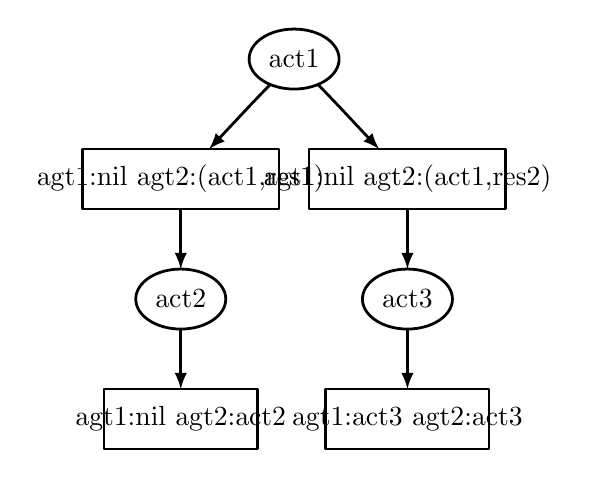
\begin{tikzpicture}[>=latex,join=bevel,scale=0.60]
  \pgfsetlinewidth{1bp}
%
\pgfsetcolor{black}
  % Edge: n1 -> n2
  \draw [->] (113bp,219bp) .. controls (104bp,210bp) and (93bp,198bp)  .. (76bp,180bp);
  % Edge: n1 -> n3
  \draw [->] (141bp,219bp) .. controls (150bp,210bp) and (161bp,198bp)  .. (178bp,180bp);
  % Edge: n4 -> n5
  \draw [->] (59bp,72bp) .. controls (59bp,64bp) and (59bp,55bp)  .. (59bp,36bp);
  % Edge: n6 -> n7
  \draw [->] (195bp,72bp) .. controls (195bp,64bp) and (195bp,55bp)  .. (195bp,36bp);
  % Edge: n2 -> n4
  \draw [->] (59bp,144bp) .. controls (59bp,136bp) and (59bp,127bp)  .. (59bp,108bp);
  % Edge: n3 -> n6
  \draw [->] (195bp,144bp) .. controls (195bp,136bp) and (195bp,127bp)  .. (195bp,108bp);
  % Node: n1
\begin{scope}
  \pgfsetstrokecolor{black}
  \draw (127bp,234bp) ellipse (27bp and 18bp);
  \draw (127bp,234bp) node {act1};
\end{scope}
  % Node: n2
\begin{scope}
  \pgfsetstrokecolor{black}
  \draw (118bp,180bp) -- (0bp,180bp) -- (0bp,144bp) -- (118bp,144bp) -- cycle;
  \draw (59bp,162bp) node {agt1:nil agt2:(act1,res1)};
\end{scope}
  % Node: n3
\begin{scope}
  \pgfsetstrokecolor{black}
  \draw (254bp,180bp) -- (136bp,180bp) -- (136bp,144bp) -- (254bp,144bp) -- cycle;
  \draw (195bp,162bp) node {agt1:nil agt2:(act1,res2)};
\end{scope}
  % Node: n4
\begin{scope}
  \pgfsetstrokecolor{black}
  \draw (59bp,90bp) ellipse (27bp and 18bp);
  \draw (59bp,90bp) node {act2};
\end{scope}
  % Node: n5
\begin{scope}
  \pgfsetstrokecolor{black}
  \draw (105bp,36bp) -- (13bp,36bp) -- (13bp,0bp) -- (105bp,0bp) -- cycle;
  \draw (59bp,18bp) node {agt1:nil agt2:act2};
\end{scope}
  % Node: n6
\begin{scope}
  \pgfsetstrokecolor{black}
  \draw (195bp,90bp) ellipse (27bp and 18bp);
  \draw (195bp,90bp) node {act3};
\end{scope}
  % Node: n7
\begin{scope}
  \pgfsetstrokecolor{black}
  \draw (244bp,36bp) -- (146bp,36bp) -- (146bp,0bp) -- (244bp,0bp) -- cycle;
  \draw (195bp,18bp) node {agt1:act3 agt2:act3};
\end{scope}
%
\end{tikzpicture}

}}{\tiny {} }%
\end{minipage}}

\caption{ A simple joint execution. Elliptical nodes are action events, box
nodes are outcome events. }


\label{fig:example-je} 
\end{figure}


Recall that a \emph{configuration} is a partial run of execution of
the prime event structure. Clearly any configuration ending in an
outcome event corresponds to a unique situation term and also a unique
history, as it is a set of alternating actions and their outcomes.

We will call a set of unordered, non-conflicting outcome events an
\emph{outcome set} and denote it $os$. A \emph{branch} is a special
case of an outcome set where every event is either in the branch,
conflicts with something in the branch, or precedes something in the
branch: \[
\forall i\in\mathcal{O}:\,\, i\in b\,\equiv\,\neg(\exists j\in b:\,\, i\oplus j\,\vee\, i\prec j)\]


A branch thus represents potential \emph{terminating} runs of the
execution. TODO: demonstrate branches in the example JE.

The \emph{histories} of an outcome set is the set of all configurations
that contain all elements of $os$, and end in an event from $os$.
By these definitions, the union of histories of all branches gives
the set of all histories that could be produced by performing the
joint execution.

A joint execution has one additional component over a standard prime
event structure: a \emph{total} order on events $<$ that is consistent
with the partial order $\prec$ induced by the enabling relation.
We call this the \emph{canonical ordering}, and it allows any branch
to be unambiguosly translated into a \emph{canonical history}. When
we come to use joint executions for planning, we will use the canonical
history to avoid having to reason about all the (potentially exponentially-many)
histories of each branch. The canonical ordering is determined by
the order of insertion of events into the structure.


\subsection{Formalities}

We introduce new sorts \noun{Event }and \noun{JointExec} to $\Lsit$,
and will collect the axioms defining joint executions in a separate
axiom set $\Dt_{je}$. Events are opaque identifiers with which a
joint execution associates a label, a set of enablers, and a set of
alternatives. For simplicity we will identify events with the integers,
although our definitions require only the successor function and ordering
relation. Labels are either \noun{Action} or \noun{Outcome} terms.


\subsubsection{Structural Axioms}

A joint execution consists of:

\begin{itemize}
\item a set of \emph{events}, which are integer ids 
\item a mapping from each event to a \emph{label}, which is either an action
or an outcome 
\item a mapping from each event to its \emph{enablers}, which is a set of
lower-numbered events 
\item a mapping from each event to its \emph{alternatives}, which is a set
of events 
\end{itemize}
As a base case, we have the empty joint execution as follows:

\[
JExec_{0}\,\isdef\, jexec(\{\},\{\},\{\},\{\})\]


The following four functions access the mappings contained in a joint
execution:\begin{gather*}
events(je)=es\,\equiv\exists ls,ns,as:\, je=jexec(es,ls,ns,as)\\
lblmap(je)=ls\,\equiv\exists es,ns,as:\, je=jexec(es,ls,ns,as)\\
ensmap(je)=ns\,\equiv\exists es,ls,as:\, je=jexec(es,ls,ns,as)\\
altsmap(je)=as\,\equiv\exists es,ls,ns:\, je=jexec(es,ls,ns,as)\end{gather*}


We also define the following shortcut accessors to get the value from
each mapping for a particular event $i$:\begin{gather*}
lbl(je,i,l)\equiv i\#l\in lblmap(je)\\
ens(je,i,ns)\equiv i\#ns\in ensmap(je)\\
alts(je,i,as)\equiv i\#as\in altsmap(je)\end{gather*}


For notational convenience we will often write these as functions,
but this should be understood as an abbreviation since not every joint
execution will contain every event. For example:\[
ens(je,i)=ns\,\isdef\,\exists ns':\, ens(je,i,ns')\wedge ns'=ns\]
 Like standard situation terms, joint executions are built up by progressively
inserting new events into an existing joint execution. First, we have
a function to get the id of the next event:\[
NextEvent(je)=max(\{0\}\cup events(je))+1\]


To add to a joint execution, we must specify the predecessor joint
execution, the label for the new event, and its set of enablers. The
set of alternatives for the new event is determined automatically
based on the required structure of the joint execution -- action events
have no alternatives, while outcome events must have as their alternatives
every other outcome event enabled by the same action.

The following predicate specifies the conditions under which such
an insertion forms a valid joint execution, according to the intuitions
discussed above:\begin{gather*}
Insert(je,lb,ns,,je')\equiv\exists i:\, NextEvent(je)=i\\
\wedge\, events(je')=events(je)\cup\{i\}\\
\wedge\, lblmap(je')=lblmap(je)\cup\{i\#lb\}\\
\wedge\, ensmap(je')=ensmap(je)\cup\{i\#ns\}\\
\wedge\left(InsertOut(je,i,lb,ns,je')\vee InsertAct(je,i,lb,ns,je')\right)\end{gather*}


Note that this is not a function, since an invalid set of enablers
could cause it to be false. Outcome events must be enabled by a single
action event, and the alternatives must be updated for all other outcome
events associated with that action:\begin{gather*}
InsertOut(je,i,lb,ns,je')\equiv\,\,\,\,\,\, IsOutcome(lb)\\
\wedge\exists j,a:\, ns=\{j\}\wedge lbl(je,j,a)\wedge IsAction(a)\\
\wedge\left(\exists allAlts:\,\forall k:\, k\in allAlts\equiv ens(je',k,\{j\})\right)\\
\wedge\forall k:\,\left[k\not\in events(je')\,\rightarrow\,\neg\exists as:\, alts(je',k,as)\right]\\
\wedge\left[ens(je',k,\{j\})\rightarrow alts(je',k,allAlts)\right]\\
\wedge\left[\neg ens(je',k,\{j\})\rightarrow\exists as:\, alts(je,k,as)\wedge alts(je',k,as)\right]\end{gather*}


Action events must be enabled by a set of outcome events and cannot
have any alternatives:\begin{gather*}
InsertAct(je,i,lb,ns,je')\equiv\,\,\,\,\,\, IsAction(lb)\\
\wedge\forall j\in ns:\,\exists lb':\, lbl(je,j,lb')\wedge IsOutcome(lb')\\
\wedge altsmap(je')=altsmap(je)\cup\{i\#\{\}\}\end{gather*}


Finally, we need a second-order induction axiom stating that the only
joint executions are those that can be constructed in this way. This
is entirely analogous to the axiom for situation terms:\begin{multline*}
\forall P:\,\left[P(JExec_{0})\wedge\forall je,je',lb,ns:\, P(je)\wedge Insert(je,lb,ns,je')\rightarrow P(je')\right]\\
\rightarrow\forall je:\, P(je)\end{multline*}


These definitions enforece the basic structure of a joint execution,
but do not constrain it to be something that could be executed in
the world -- for example, outcomes can be enabled by actions that
will never actually produce that outcome. Like situation terms, we
focus first on getting the appropriate structure, and then specify
additional conditions that joint executions must satisify in order
to be legal in the real world.

Note that we have placed an important restriction on the ordering
of events -- if $i<j$ according to the total ordering over the integers,
then it is not possible for $i$ to be enabled by $j$. This does
not result in a lack of expressiveness, since if we want $i$ to be
enabled by $j$, then $j$ must not be enabled by $i$ and we can
simply give $j$ the lower event number.

Now, let us define the \emph{preceeds} and \emph{conflicts} relations
in terms of enablers and alternatives. We will write these as binary
infix operators $\prec_{je}$ and $\oplus_{je}$. The precedence relation
is defined as a transitive closure over enablers:\begin{multline*}
\forall P,i,j:\left[\left(i\in ens(je,j)\,\rightarrow P(i,j)\right)\,\wedge\,\left(\forall k:\, P(i,k)\wedge k\in ens(je,j)\,\rightarrow\, P(i,j)\right)\right]\\
\rightarrow\left(P(i,j)\rightarrow i\prec_{je}j\right)\end{multline*}


The conflict relation is defined so that $i\oplus j$ if they have
altnerative predecessors:\begin{multline*}
\forall P,i,j:\,\left[\left(i\in alts(je,j)\,\rightarrow P(i,j)\right)\right.\\
\left.\wedge\,\left(\forall i',j':\, P(i',j')\wedge i'\preceq_{je}i\wedge j'\preceq_{je}j\,\rightarrow\, P(i,j)\right)\right]\\
\rightarrow\left(P(i,j)\rightarrow i\oplus_{je}j\right)\end{multline*}


These axioms suffice to give an account of joint executions as prime
event structures as defined in \citep{npw79event_structures}.


\subsubsection{Additional Notions}

We also require some additional definitions and notation that is not
typically found in the literature on prime event structures, in order
to related joint executions back to the existing concepts of the situation
calculus.

An \emph{outcome set} is a set of unordered non-conflicting outcome
events; that is, a set of events satisfying:\begin{multline*}
OutcomeSet(je,os)\,\equiv\,\forall i,j\in os:\, IsOutcome(lbl(je,i)\\
\wedge IsOutcome(lbl(je,j)\\
\wedge\,\neg(i\oplus_{je}j)\,\wedge\, i\not\prec_{je}j\,\wedge\, j\not\prec_{je}\, j\end{multline*}


An outcome set identifies a family of potential partial runs of the
execution. We can generate these histories by recursively selecting
an event that does not conflict with anything in $os$ and is enabled
given what we have performed so far:

TODO

An outcome set $os$ \emph{covers} a set \emph{$os'$,} denoted by
$os\sqsubseteq_{je}os'$, if every event in $os$ is either also in
$os'$, or precedes something in $os'$. Every history in $hists(os')$
will have a prefix in $hists(os)$. This defines a partial ordering
on outcome sets:\[
os\sqsubseteq_{je}os'\,\equiv\,\forall i\in os:\,\,\exists i'\in os':\,\, i\preceq_{je}i'\]


A \emph{branch}, denoted $b$, is a special case of an outcome set
that meets the following additional requirement:\[
Branch(je,b)\,\equiv\,\forall i\in events(je):\, i\in b\,\equiv\,\neg(\exists i'\in b:\,\, i\oplus i'\,\vee\, i\prec i')\]



\subsection{Feasible Joint Executions}

We now impose two restrictions on joint executions to ensure that
they are \emph{feasible} -- that the agents will actually be able
to perform them in the world.

The first restriction corresponds to the idea of \emph{knowing when}
to perform an action. If an action event $i$ is enabled by an outcome
event $j$ produced by another agent, the agent performing $i$ must
be able to observe the occurrence of $j$. Otherwise, it has no way
of synchronizing its actions with those of its teammate. Let $actor(i)$
be the agent responsible for performing an action event $i$, then
we require that:\[
\forall i,j\in events(je):\, IsAction(lbl(je,i))\,\wedge j\in ens(je,i)\rightarrow\, lbl(je,j)[actor(je,i)]\neq\{\}\]


The second restriction corresponds to the idea of \emph{knowing what}
action to perform. For a given event $i$, define the enabling views
of $i$ are all views in in which the agent responsible for $i$ could
be required to execute it:\[
EnablingView(je,i,v)\equiv\exists agt,h:\, actor(je,i)=agt\wedge Hist(je,ens(je,i),h)\wedge View(agt,h)=v\]


This definition gives all the possible views of $agt$ in which event
$i$ is enabled, and so the agent is required to perform action $lbl(je,i)$.
Since the agent has only a local viewpoint, it is possible that some
other outcome set can produce an identical view. Say that two outcome
sets overlap, denoted $Overlaps(je,agt,os,os')$, if they could produce
an identical local history for a given agent:\[
\exists v:\, EnablingView(je,view(agt,hists(e_{1}))\,\cap\, view(agt,hists(e_{2}))\,\neq\varnothing\]


TODO: formulate this properly

Then the \emph{minimal overlapping set} for $e_{1}$, from the perspective
of $agt$, is the set of all $e_{2}$ satisfying:\begin{multline*}
e_{2}\in minovlp(agt,e_{1})\,\equiv\\
ovlaps(agt,e_{1},e_{2})\wedge\neg\exists e_{3}\left[ovlaps(agt,e_{1},e_{3})\wedge e_{3}\sqsubset e_{2}\right]\end{multline*}


This captures all outcome sets that the agent could potentially confuse
for $e_{1}$. To ensure there is no confusion about whether an action
is enabled, for each $i\in\mathcal{A}$, every $e$ in the minimal
overlapping set of $ens(i)$ for $actor(i)$ must enable an event
$i'$ with identical action $\gamma(i')=\gamma(a)$. Formally:\begin{multline*}
\forall e\in minovlp(actor(i),ens(i)):\,\\
\exists i':\,\gamma(i')=\gamma(i)\,\wedge\, ens(i')=e\end{multline*}
 This ensures that the agent's local information is enough to know
when it should perform an action. While it may not know precisely
which \emph{event} is enabled, it will know enough to determine the
specific \emph{action} that it must perform.

Finally, we say a joint execution is feasible if it meets both these
conditions:\[
Feasible(je)\,\isdef\, KnowsWhat(je)\wedge KnowsWhen(je)\]



\subsection{Legal Joint Executions}

We call a branch of a joint execution \emph{legal} if every history
of that branch corresponds to a legal situation:\[
Legal(je,b)\,\isdef\,\forall h\in Hists(je,b):\,\exists s:\, Legal(s)\wedge History(s)=h\]


In general, the agents will not have enough information to determine
whethe a particular branch is legal, since this would imply that they
already know what sensing results will occur.

We will call a joint execution \emph{legal} if it contains a legal
branch:\[
Legal(je)\,\isdef\,\exists b:\, Branch(je,b)\wedge Legal(b)\]


This definition does not require that we establish \emph{which} branch
is legal, only that we are able to prove that \emph{some} branch must
be legal. It is also permissive, in that is permits redundant branches
that can never be legal. Since these branches will not actually be
taken at execution time, this permissiveness will not affect the agent's
ability to carry out the plan.


\subsection{Planning with Joint Executions}

Finally, we are in a position to plan the cooperative execution of
a shared MIndiGolog program using these structures. Consider first
\emph{offline} planning in the style ConGolog and the original Golog.
The agents need to find a feasible, legal joint execution such that
for every branch, if that branch is legal, then it will form a legal
execution of the program:\begin{multline*}
\Dt\cup\Dt_{mgolog}\cup\Dt_{je}\models\exists je:\, Legal(je)\wedge Feasible(je)\wedge\\
\forall b:\, Branch(je,b)\wedge Legal(je,b)\,\rightarrow\,\left[\forall s:\, Sit(je,b,s)\rightarrow\Do(\delta,S_{0},s)\right]\end{multline*}


This captures a pair of soundness and completeness requirements. For
soundness we require that for every branch of the joint execution,
\emph{if} that branch is legal then it will be a legal execution of
the program. For completeness, we assert that there must be some legal
branch.


\subsection{Summary\label{sec:JointExec:Summary}}

In this section we have defined a \emph{joint execution} as a prime
event structure with some additional restrictions. We contend that
such structures are highly suitable for planning the actions to be
performed by a team in service of some shared task, such as executing
a shared Golog program.

On one hand, joint executions are restricted enough to be practical
for such use. Prime event structures are purely reactive (equivalent
to a kind of finite automaton) and can be executed by the agents without
further deliberation. They are restricted to ensure that whenever
an agent is required to perform an action, it is able to determine
this using only its local information. Each branch of execution can
be easily converted into a situation term for the purposes of reasoning,
and can be extended one action at a time.

Joint executions are also significantly more flexible than previous
approaches. They allow independent actions to be performed without
synchronization, in any order. The agents need never know precisely
what actions have been executed, only those that enable them to perform
their next action. Synchronization is automatically achieved when
required by explicitly reasoning about what actions each agent can
observe, rather than requiring that all actions be public.

To demonstrate the utility of these structures, we have implemented
an interpreter for multi-agent ConGolog programs that produces joint
executions as its output. In the next section, we highlight the key
aspects of our implementation and give an example of the output it
produces.


\section{Implementation\label{sec:JointExec:Implementation}}

While these structures so far allow provide a powerful formal account
of execution planning in multi-agent domains, they are not suitable
for an effective implementation. In order to verify that a joint execution
is legal, it is necessary to examine every possible history of every
brach in the execution. Since it is a partially-ordered structure
there is a potentially exponential number of histories for every branch. 


\subsection{Independent Actions\label{sec:JointExec:IndepActs}}

As discussed in Section \ref{sec:Background}, posing queries in the
situation calculus requires a full situation term, which means a total
order on all actions that have occurred. The first step towards providing
only a \emph{partial} order on the actions to be performed is, therefore,
to capture the conditions under which actions can be performed out
of order without invalidating the results of the reasoning process.

Define \emph{independent} actions, identified by $indep(a_{1},a_{2},s)$,
as those that can be performed in either order, or even concurrently,
without affecting what holds in the resulting situation. Formally,
they must satisfy the following restrictions (where $\mathcal{P}$
and $\mathcal{F}$ are meta-variables ranging over predicate and functional
fluents respectively):

\begin{itemize}
\item $\mathcal{D}\,\models\, Poss(a_{1},s)\equiv Poss(a_{1},do(a_{2},s))$
and vice-versa 
\item $\mathcal{D}\,\models\, Out(a_{1},s)=Out(a_{1},do(a_{2},s))$ and
vice-versa 
\item $\mathcal{D}\,\models\,\mathcal{P}(do(a_{1},do(a_{2},s)))\equiv\mathcal{P}(do(a_{2},do(a_{1},s)))$\\
 for all predicate fluents $\mathcal{P}(s)$ 
\item $\mathcal{D}\,\models\,\mathcal{F}(do(a_{1},do(a_{2},s)))=\mathcal{F}(do(a_{2},do(a_{1},s)))$\\
 for all functional fluents $\mathcal{F}(s)$ 
\end{itemize}
Whether actions are independent can be deduced from the description
of the action theory, or (as currently in our implementation) indicated
explicitly by the programmer.

We assume that the planning system has some way of identifying independent
actions. Two histories $\sigma_{1}$ and $\sigma_{2}$ are called
\emph{equivalent} if they are identical up to the ordering of independent
actions: they contain the same set of $(a,Out(a,s))$ pairs, and whenever
two such pairs occur in a different order in $\sigma_{1}$ than in
$\sigma_{2}$ the actions are independent. Two histories $\sigma_{1}$
and $\sigma_{2}$ are \emph{compatible for $a$} if they are equivalent
after removing all actions that are independent of $a$. We then have
the following properties of histories:

\begin{thm}
\label{thm:equiv-holds}For equivalent histories $\sigma_{1}$ and
$\sigma_{2}$:\[
\mathcal{D}\,\models\,\mathbf{holds}[\phi,\sigma_{1}]\,\,\equiv\,\,\mathbf{holds}[\phi,\sigma_{2}]\]

\end{thm}
\begin{proof}
A straightforward case analysis on the definition of the regression
operator. 
\end{proof}
\begin{thm}
\label{thm:equiv-legal}For equivalent histories $\sigma_{1}$ and
$\sigma_{2}$:\[
\mathcal{D}\,\models\,\mathbf{legal}[\sigma_{1}]\,\,\equiv\,\,\mathbf{legal}[\sigma_{2}]\]

\end{thm}
\begin{proof}
Using theorem \ref{thm:equiv-holds}, and invariance of $Poss$ and
$Out$ when transposing independent actions. 
\end{proof}
\begin{thm}
\label{thm:equiv-compat}For histories $\sigma_{1}$ and $\sigma_{2}$
compatible for $a$:\begin{gather*}
\mathcal{D}\,\models\,\mathbf{holds}[Poss(a),\sigma_{1}]\,\,\equiv\,\,\mathbf{holds}[Poss(a),\sigma_{2}]\\
\mathcal{D}\,\models\,\mathbf{holds}[Out(a)=r,\sigma_{1}]\,\,\equiv\,\,\mathbf{holds}[Out(a)=r,\sigma_{2}]\end{gather*}

\end{thm}
\begin{proof}
Using Theorem \ref{thm:equiv-holds}, and the fact that the removed
actions do not affect the preconditions or outcome of $a$. 
\end{proof}

\subsection{Canonical Joint Executions}

We now impose several restrictions on the structure of a joint execution,
to ensure they are suitable for representing the actions to be performed
by a team of agents.

\textbf{(R1) Independent events have independent actions}\\
 If the execution allows two action events to occur in either order,
then the corresponding actions must be independent. Formally, for
each $i_{1},i_{2}\in\mathcal{A}$:\[
i_{1}\prec i_{2}\,\vee\, i_{2}\prec i_{1}\,\vee\, i_{1}\#i_{2}\,\vee\, indep(\gamma(i_{1}),\gamma(i_{2}))\]


This restriction is key to the power of joint executions. It implies
that for every branch $b$, all histories in $hists(b)$ are equivalent.
By Theorem \ref{thm:equiv-holds} we can use the canonical history
for planning purposes, and be assured that the same fluents will hold
regardless of the specific order in which actions are executed. More
generally, it ensures that all histories in $hists(ens(i))$ are compatible
for $\gamma(i)$. By Theorem \ref{thm:equiv-compat} we can safely
use $hist(ens(i))$ to reason about the preconditions and outcomes
of $\gamma(i)$ using standard techniques.


\subsection{Planning Loop}

We have extended the implementation of a MIndiGolog execution planner
from Chapter \ref{ch:mindigolog} to utilise joint executions.

To make things more concrete, Figure \ref{fig:plan-output} shows
the output of our system when run on the $MakeSalad$ example of Figure
\ref{fig:makesalad-program}. Since all actions in this program have
a single outcome, the outcome events have been suppressed for brevity.

In this domain there are three agents, but only two chopping boards
are available. The agents must therefore synchronize their use of
these resources. Actions are taken to be independent if they deal
with different objects. As seen in Figure \ref{fig:plan-output},
the use of a partial order structure facilitates parallelism between
the agents, with each processing a different ingredient and only synchronizing
on the availability of the required resources. There is no need for
processing actions, such as $mix$ and $chop$, to be publicly observable.
This execution is maximally concurrent given the constraints of the
domain, and is clearly a significant improvement over totally ordered
sequences of actions as produced by existing systems.

In the following subsections, we briefly highlight some key aspects
of our implementation.


\subsection{Program Steps}

While the ability to determine whether actions are independent is
necessary in constructing partially-ordered executions of a ConGolog
program, it is not sufficient. Actions might have an order imposed
on them directly by the program (for example by the sequence construct
$a_{1};a_{2}$). The program may require that some additional conditions
are true immediately prior to executing an action (for example to
satisfy a test construct $\phi?$), which could be falsified by an
otherwise independent action.

To ensure that the dependencies between actions reflect the needs
of the program being executed, we augment our implementation of the
$Trans$ predicate to keep additional information about what transitions
were made. A \emph{step} object has the following attributes:

\begin{itemize}
\item action: the action performed in that step, or $nil$ if it is an internal
program transition 
\item test: an additional fluent formula that must hold immediately before
performing the step 
\item thread: a sequence of 'l' and 'r' characters indicating the concurrent
thread in which the step is performed 
\item outcome: the outcome of performing the action. 
\end{itemize}
%
\begin{figure}
\framebox{%
\begin{minipage}[t][1\totalheight]{1\columnwidth}%
\textsf{\textbf{\tiny 
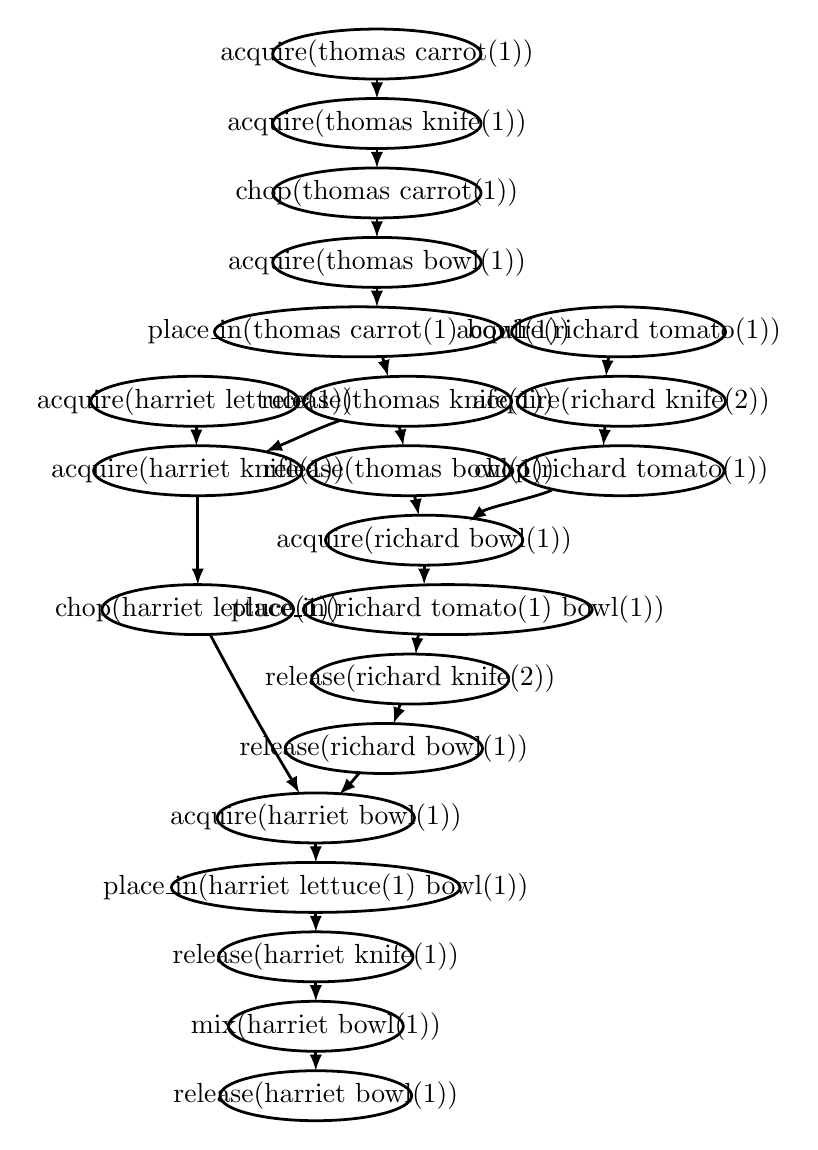
\begin{tikzpicture}[>=latex,join=bevel,scale=0.50]
  \pgfsetlinewidth{1bp}
%
\pgfsetcolor{black}
  % Edge: n0 -> n6
  \draw [->] (196bp,750bp) .. controls (196bp,749bp) and (196bp,748bp)  .. (196bp,736bp);
  % Edge: n2 -> n8
  \draw [->] (363bp,550bp) .. controls (363bp,549bp) and (362bp,547bp)  .. (361bp,536bp);
  % Edge: n6 -> n10
  \draw [->] (196bp,700bp) .. controls (196bp,699bp) and (196bp,698bp)  .. (196bp,686bp);
  % Edge: n8 -> n12
  \draw [->] (360bp,500bp) .. controls (360bp,499bp) and (360bp,497bp)  .. (359bp,486bp);
  % Edge: n10 -> n14
  \draw [->] (196bp,650bp) .. controls (196bp,649bp) and (196bp,648bp)  .. (196bp,636bp);
  % Edge: n14 -> n16
  \draw [->] (196bp,600bp) .. controls (196bp,599bp) and (196bp,598bp)  .. (196bp,586bp);
  % Edge: n16 -> n18
  \draw [->] (200bp,550bp) .. controls (200bp,549bp) and (201bp,547bp)  .. (204bp,536bp);
  % Edge: n18 -> n20
  \draw [->] (212bp,500bp) .. controls (212bp,499bp) and (213bp,497bp)  .. (215bp,486bp);
  % Edge: n18 -> n22
  \draw [->] (169bp,504bp) .. controls (152bp,498bp) and (138bp,491bp)  .. (116bp,482bp);
  % Edge: n4 -> n22
  \draw [->] (66bp,500bp) .. controls (66bp,499bp) and (66bp,498bp)  .. (66bp,486bp);
  % Edge: n20 -> n24
  \draw [->] (223bp,450bp) .. controls (223bp,449bp) and (224bp,447bp)  .. (226bp,436bp);
  % Edge: n12 -> n24
  \draw [->] (322bp,454bp) .. controls (308bp,448bp) and (276bp,442bp)  .. (263bp,432bp);
  % Edge: n22 -> n26
  \draw [->] (67bp,450bp) .. controls (67bp,435bp) and (67bp,413bp)  .. (67bp,386bp);
  % Edge: n24 -> n28
  \draw [->] (230bp,400bp) .. controls (230bp,399bp) and (230bp,398bp)  .. (230bp,386bp);
  % Edge: n28 -> n30
  \draw [->] (226bp,350bp) .. controls (226bp,349bp) and (225bp,347bp)  .. (224bp,336bp);
  % Edge: n30 -> n32
  \draw [->] (213bp,300bp) .. controls (212bp,299bp) and (212bp,297bp)  .. (208bp,286bp);
  % Edge: n32 -> n34
  \draw [->] (184bp,251bp) .. controls (181bp,248bp) and (179bp,245bp)  .. (169bp,235bp);
  % Edge: n26 -> n34
  \draw [->] (76bp,350bp) .. controls (88bp,327bp) and (111bp,285bp)  .. (132bp,250bp) .. controls (133bp,248bp) and (134bp,247bp)  .. (140bp,236bp);
  % Edge: n34 -> n36
  \draw [->] (152bp,200bp) .. controls (152bp,199bp) and (152bp,198bp)  .. (152bp,186bp);
  % Edge: n36 -> n38
  \draw [->] (152bp,150bp) .. controls (152bp,149bp) and (152bp,148bp)  .. (152bp,136bp);
  % Edge: n38 -> n40
  \draw [->] (152bp,100bp) .. controls (152bp,99bp) and (152bp,98bp)  .. (152bp,86bp);
  % Edge: n40 -> n42
  \draw [->] (152bp,50bp) .. controls (152bp,49bp) and (152bp,48bp)  .. (152bp,36bp);
  % Node: n0
\begin{scope}
  \pgfsetstrokecolor{black}
  \draw (196bp,768bp) ellipse (75bp and 18bp);
  \draw (196bp,768bp) node {acquire(thomas carrot(1))};
\end{scope}
  % Node: n2
\begin{scope}
  \pgfsetstrokecolor{black}
  \draw (370bp,568bp) ellipse (77bp and 18bp);
  \draw (370bp,568bp) node {acquire(richard tomato(1))};
\end{scope}
  % Node: n4
\begin{scope}
  \pgfsetstrokecolor{black}
  \draw (65bp,518bp) ellipse (75bp and 18bp);
  \draw (65bp,518bp) node {acquire(harriet lettuce(1))};
\end{scope}
  % Node: n6
\begin{scope}
  \pgfsetstrokecolor{black}
  \draw (196bp,718bp) ellipse (75bp and 18bp);
  \draw (196bp,718bp) node {acquire(thomas knife(1))};
\end{scope}
  % Node: n8
\begin{scope}
  \pgfsetstrokecolor{black}
  \draw (372bp,518bp) ellipse (75bp and 18bp);
  \draw (372bp,518bp) node {acquire(richard knife(2))};
\end{scope}
  % Node: n10
\begin{scope}
  \pgfsetstrokecolor{black}
  \draw (196bp,668bp) ellipse (75bp and 18bp);
  \draw (196bp,668bp) node {chop(thomas carrot(1))};
\end{scope}
  % Node: n12
\begin{scope}
  \pgfsetstrokecolor{black}
  \draw (372bp,468bp) ellipse (74bp and 18bp);
  \draw (372bp,468bp) node {chop(richard tomato(1))};
\end{scope}
  % Node: n14
\begin{scope}
  \pgfsetstrokecolor{black}
  \draw (196bp,618bp) ellipse (75bp and 18bp);
  \draw (196bp,618bp) node {acquire(thomas bowl(1))};
\end{scope}
  % Node: n16
\begin{scope}
  \pgfsetstrokecolor{black}
  \draw (183bp,568bp) ellipse (104bp and 18bp);
  \draw (183bp,568bp) node {place\_in(thomas carrot(1) bowl(1))};
\end{scope}
  % Node: n18
\begin{scope}
  \pgfsetstrokecolor{black}
  \draw (218bp,518bp) ellipse (75bp and 18bp);
  \draw (218bp,518bp) node {release(thomas knife(1))};
\end{scope}
  % Node: n20
\begin{scope}
  \pgfsetstrokecolor{black}
  \draw (219bp,468bp) ellipse (73bp and 18bp);
  \draw (219bp,468bp) node {release(thomas bowl(1))};
\end{scope}
  % Node: n22
\begin{scope}
  \pgfsetstrokecolor{black}
  \draw (67bp,468bp) ellipse (75bp and 18bp);
  \draw (67bp,468bp) node {acquire(harriet knife(1))};
\end{scope}
  % Node: n24
\begin{scope}
  \pgfsetstrokecolor{black}
  \draw (230bp,418bp) ellipse (71bp and 18bp);
  \draw (230bp,418bp) node {acquire(richard bowl(1))};
\end{scope}
  % Node: n26
\begin{scope}
  \pgfsetstrokecolor{black}
  \draw (67bp,368bp) ellipse (69bp and 18bp);
  \draw (67bp,368bp) node {chop(harriet lettuce(1))};
\end{scope}
  % Node: n28
\begin{scope}
  \pgfsetstrokecolor{black}
  \draw (247bp,368bp) ellipse (104bp and 18bp);
  \draw (247bp,368bp) node {place\_in(richard tomato(1) bowl(1))};
\end{scope}
  % Node: n30
\begin{scope}
  \pgfsetstrokecolor{black}
  \draw (220bp,318bp) ellipse (71bp and 18bp);
  \draw (220bp,318bp) node {release(richard knife(2))};
\end{scope}
  % Node: n32
\begin{scope}
  \pgfsetstrokecolor{black}
  \draw (201bp,268bp) ellipse (71bp and 18bp);
  \draw (201bp,268bp) node {release(richard bowl(1))};
\end{scope}
  % Node: n34
\begin{scope}
  \pgfsetstrokecolor{black}
  \draw (152bp,218bp) ellipse (71bp and 18bp);
  \draw (152bp,218bp) node {acquire(harriet bowl(1))};
\end{scope}
  % Node: n36
\begin{scope}
  \pgfsetstrokecolor{black}
  \draw (152bp,168bp) ellipse (104bp and 18bp);
  \draw (152bp,168bp) node {place\_in(harriet lettuce(1) bowl(1))};
\end{scope}
  % Node: n38
\begin{scope}
  \pgfsetstrokecolor{black}
  \draw (152bp,118bp) ellipse (70bp and 18bp);
  \draw (152bp,118bp) node {release(harriet knife(1))};
\end{scope}
  % Node: n40
\begin{scope}
  \pgfsetstrokecolor{black}
  \draw (152bp,68bp) ellipse (63bp and 18bp);
  \draw (152bp,68bp) node {mix(harriet bowl(1))};
\end{scope}
  % Node: n42
\begin{scope}
  \pgfsetstrokecolor{black}
  \draw (152bp,18bp) ellipse (69bp and 18bp);
  \draw (152bp,18bp) node {release(harriet bowl(1))};
\end{scope}
%
\end{tikzpicture}

}}%
\end{minipage}}

\caption{ Joint execution for $MakeSalad(bowl(1))$, showing significant concurrency
between agents }


\label{fig:plan-output} 
\end{figure}


We call a sequence of such steps a \emph{run}, which can be converted
to a history by taking just the action and outcome attributes. The
procedure implementing $Trans$ takes a program and a run as input,
returning a new program and new step of execution. As an example consider
the code in Figure \ref{fig:trans-code}, implementing the test operator
and the concurrency operator from equation \ref{eqn:trans_conc_orig}.

%
\begin{figure}
\framebox{%
\begin{minipage}[t][1\totalheight]{1\columnwidth}%
{\scriptsize \verbatiminput{listings/jointexec/ConGolog.oz}}%
\end{minipage}}

\caption{ Partial code for $Trans$ predicate }


\label{fig:trans-code} 
\end{figure}


Note that whenever the procedure descends through the left side of
a concurrency operator it pushes an 'l' onto the step's {}``thread''
attribute, and each descent through the right side pushes an 'r'.
Two steps can be said to come from different threads as long as neither
{}``thread'' attribute is a prefix of the other.

We say that two steps are \emph{ordered} if any of the following holds:
their action terms are not independent; ones thread is a prefix of
the other; ones action falsifies the test condition associated with
the other. When building a joint execution, ordered steps are forced
to be executed in the order they were generated by the planner, while
unordered steps may be performed independently.


\subsection{Planning Procedure}

The code for planning a joint execution from a given ConGolog program
is shown in Figure \ref{fig:planning-code}. The main procedure is
$MakePlan$, a recursive procedure that operates on a list of branches-in-progress
of the form $(D,R,B)$. Here $B$ is a branch in the joint execution
under construction, $D$ is the program remaining to be executed on
that branch, and $R$ is the run of program steps performed on that
branch so far.

%
\begin{figure}
\framebox{%
\begin{minipage}[t][1\totalheight]{1\columnwidth}%
{\scriptsize \verbatiminput{listings/jointexec/Planner.oz}}%
\end{minipage}}

\caption{ Code for main planning loop }


\label{fig:planning-code} 
\end{figure}


%
\begin{figure}
\framebox{%
\begin{minipage}[t][1\totalheight]{1\columnwidth}%
{\scriptsize \verbatiminput{listings/jointexec/psearch.oz}}%
\end{minipage}}

\caption{ Code to run planning procedure in parallel }


\label{fig:parallel-search} 
\end{figure}


Each iteration of the planning loop proceeds as follows. The procedure
$FindOpenBranch$ updates each branch to account for events that were
added since it was last processed (some may have been added automatically
to satisfy restriction (R5)), then searches the list to find a branch
for which $Final(D,R)$ does not hold. If all branches are final,
planning can terminate. Otherwise, the procedure $FindTrans1$ is
called to find a new step of execution for that branch. The action
is inserted into the joint execution, which returns a list of new
branches, one for each possible outcome of the action. Each of these
outcomes is added to the list of branches, and the loop is started
again.

Of particular interest is the procedure $FindTrans1$, which uses
the encapsulated search functionality of Mozart to yield possible
next steps according to an estimate of their potential for concurrency.
The procedure $LP.yieldOrdered$ yields the solutions of the given
search context, sorted using the procedure $CompareSteps$. This procedure
(not shown) gives preference to steps that can be performed concurrently
with as many existing actions as possible.


\subsection{Distributing the Planning Workload}

A primary motivation in using Mozart/Oz for our implementation is
its strong support for distributed logic programming. Utilizing Mozart's
parallel search functionality \citep{Schulte00constraint_services},
the planning workload can be transparently distributed between the
agents in the team.

Figure \ref{fig:parallel-search} shows the necessary code, which
should be executed by one of the agents. The planning procedure is
encapsulated in a \emph{functor}, a portable code object. A parallel
search object is then created, which uses an ssh connection to spawn
remote computations on each of the three agents (identified by their
DNS names). The object is asked to provide a single solution, which
is then written to a file in the graphviz 'dot' format for display
(resulting in Figure \ref{fig:plan-output}).

For the simple example shown in this chapter, parallel plan search
does not demonstrate a significant time saving since almost no backtracking
is required to reach a solution. For more difficult problems, significant
gains can be expected.


\section{Discussion\label{sec:JointExec:Discussion}}

An alternate approach to the problem of partial observability is the
language TeamGolog developed in \citep{farinelli07team_golog}, where
agents explicitly synchronize through communication and a shared state.
By contrast, our approach constructs synchronization implicitly by
reasoning about the actions that can be observed by each agent. This
has the advantage of requiring no changes to the form or semantics
of the agents' control program, but the disadvantage that joint execution
construction may fail if too many actions are unobservable. It would
be interesting to combine these approaches by automatically incorporating
explicit communication when implicit synchronization is not possible.

There is, of course, an extensive body of work on partial-order planning
in the context of goal-based planning. Unsurprisingly, the joint execution
structure we develop here has deep similarities to the structures
used in conditional partial-order planners such as \citep{peot92conditional_nonlinear}.
It is, however, intentionally specific to the situation calculus.
We make no use of many concepts common in partial-order goal-based
planning (causal links, threats, conflicts, etc) because we do not
deal explicitly with goals, but with steps generated by an underlying
transition semantics. Our approach can be considered roughly equivalent
to \emph{deordering} of a totally-ordered plan as described in \citep{backstrom99reordering},
except performed during plan construction rather than as a post-processing
step.

loops: \citep{levesque96what_is_planning,levesque05planning_with_loops}




\chapter{Property Persistence}

\label{ch:persistence}

This chapter develops a new reasoning technique for the situation
calculus that can handle certain types of universally-quantified query.
As discussed briefly at the end of Chapter \ref{ch:observations},
for an agent in an asynchronous domain to reason about the world based
on its local information, it needs to pose queries that universally
quantify over situation terms. Unfortunately such queries cannot be
handled using the regression operator, and have thus far been beyond
the reach of automated reasoning systems for the situation calculus.

In this chapter we study a subset of universally-quantified queries
that we refer to as \emph{property persistence queries}. We introduce
an approach to reasoning that is similar in spirit to the standard
regression operator: transform the query into a form more amenable
to automated reasoning. A new operator $\Pst_{\Dt}$ is defined, such
that $\phi$ persists in $s$ if and only if $\mathcal{P}_{\mathcal{D}}(\phi)$
holds in $s$. We term this the \emph{persistence condition} of $\phi$,
and show how to calculate it in a form suitable for effective automated
reasoning. The resulting formula can be used in combination with standard
regression-based reasoning techniques.

The chapter proceeds as follows: after some more detailed background
material on inductive reasoning in the situation calculus in Section
\ref{sec:Persistence:Background}, we formally define the class of
property persistence queries in Section \ref{sec:Persistence:Definitions},
along with several examples of practical queries that are of this
form. Section \ref{sec:Persistence:Condition} defines the persistence
condition operator and demonstrates that it is the equivalent to the
result of a meta-level fixpoint calculation. Section \ref{sec:Persistence:Calculating}
presents a simple iterative algorithm for calculating the persistence
condition, and disucsses its correctness, completeness, and effectiveness.
We conclude with a brief discussion in Section \ref{sec:Persistence:Discussion}.


\section{Background\label{sec:Persistence:Background}}

While there is a rich and diverse literature base for the situation
calculus, there appears to have been little work dealing with universally
quantified queries. The work of \citet{Reiter93proving} shows how
to handle such queries manually using an appropriate instantiation
of the second-order induction axiom, but makes no mention of automating
this reasoning.

Other work considering queries that universally quantify over situations
seems to focus exclusively on verifying state constraints. These are
uniform formulae that must hold in every possible situation, a highly
specialized form of the more general persistence queries we define
in this chapter. The work of \citet{Lin94-StateConstraints} shows
that the induction axiom can be {}``compiles away'' when verifying
a state constraint, by means of the following equivalence:\begin{gather*}
\Dt\,\models\,\phi[S_{0}]\rightarrow\left(\forall s:\, S_{0}\leq s\rightarrow\phi[s]\right)\\
\mathit{iff}\\
\mathcal{D}_{una}\models\forall s,a:\,\phi[s]\wedge\mathcal{R}_{\mathcal{D}}[Poss(a,s)]\,\rightarrow\,\mathcal{R}_{\mathcal{D}}[\phi[do(a,s)]]\end{gather*}
 Here the background theory contains only the unique names axioms
for action and is written $\Dt_{una}$/ Verification of a state constraint
can thus be reduced to reasoning about a universally quantified uniform
formula using only the background theory, a comparatively straightforward
reasoning task which we call \emph{static domain reasoning}. Verification
of state constraints has also also approached by \citet{bertossi96automating},
who develop a system for automatic constraint verification based on
an induction theorem prover.

However, there are many issues that are not addressed work specific
to staet constraints. What if we are interested in the future of some
arbitrariy situation $\sigma$, rather than only $S_{0}$? What if
want to restrict future actions according to an arbitrary action description
predicate? Can we integrate a method for handling universally-quantified
queries with existing regression techniques? Our treatment of property
persistence can provide a concrete basis for these considerations,
and is hence significantly more general than this existing work.

Another field that deals with induction over situations is the verification
of ConGolog programs. TODO {[}evgenia's paper] show how to formulate
various safety, liveness, and starvation properties of a ConGolog
program as fixpoint queries in second-order logic. A preliminary model-checker
capable of verifying these properties is described in {[}TODO: evgenia's
\emph{other} paper]. \citet{classen08golog_properties} develop a
logic of ConGolog programs in $\mathcal{ES}$, a variant of the situation
calculus based on modal logic. They demonstrate the properties of
a program can be verified using an iterative fixpoint computation
similar to the one we propose in this chapter.

As we shall see, property persistence queries are equivalent to a
particular kind of safety property of a ConGolog program, so our work
is in a sense \emph{less} general than that described above. However,
the ConGolog verifiers are designed to operate in isolation, while
we seek a method of handling universally-quantified queries that can
integrate directly with the existing meta-theorical reasoning machinery
of the situation calculus, in particular with the regression operator.


\section{Property Persistence Queries\label{sec:Persistence:Definitions}}

To begin, let us formally define the kinds of query that will be approached
in this chapter. Given some property $\phi$ and situation $\sigma$,
a \emph{property persistence query} asks whether $\phi$ will hold
in all situations in the future of $\sigma$: \[
\mathcal{D}\models\forall s:\,\sigma\sqsubseteq s\,\rightarrow\,\phi[s]\]


More generally, one may wish to limit the futures under consideration
to those brought about by a actions satisfying a certain action description
predicate $\alpha$, which is easily accomplished using $\leq_{\alpha}$
macro. Thus, we have the following definition of persistence queries:

\begin{defnL}
[{Property~Persistence~Query}] Let $\phi$ be a uniform
formula, $\alpha$ an action description predicate, and $\sigma$
a situation term. Then a property persistence query is a query of
the form:\[
\mathcal{D}\models\forall s:\,\sigma\le_{\alpha}s\rightarrow\phi[s]\]

\end{defnL}
In words, a persistence query states that {}``$\phi$ holds in $\sigma$,
and given that all subsequent actions satisfy $\alpha$, $\phi$ will
continue to hold''. For succinctness we will hencefore describe this
as {}``$\phi$ persists under $\alpha$''. Queries of this form
are involved in many useful reasoning tasks, of which the following
are a small selection:\\


\textbf{Goal Impossibility:} Given a goal $G$, establish that there
is no legal situation in which that goal is satisfied:\[
\mathcal{D}\models\forall s:\, S_{0}\leq_{Legal}s\rightarrow\neg G[s]\]


\textbf{Goal Futility:} Given a goal $G$ and situation $\sigma$,
establish that the goal cannot be satisfied in any legal future situation
from $\sigma$:\[
\mathcal{D}\models\forall s:\,\sigma\leq_{Legal}s\rightarrow\neg G[s]\]


Note how this differs from goal impossibility: while the agent may
have initially been able to achieve its goal, the actions that have
subsequently been performed have rendered the goal unachievable. Agents
would be well advised to avoid such situations.\\


\textbf{Checking State Constraints:} Given a state constraint $SC$,
show that the constraint holds in every legal situation:\[
\Dt\models\forall s:\, S_{0}\leq_{Legal}s\rightarrow SC[s]\]
 Indeed, this can be seen as a variable of goal impossibility, by
showing that the constraint can never be violated.\\


\textbf{Need for Cooperation:} Given an agent $agt$, goal $G$ and
situation $\sigma$, establish that no sequence of actions performed
by that agent can achieve the goal:\[
\mathcal{D}\models\forall s:\,\sigma\leq_{actor=agt}s\rightarrow\neg G[s]\]
 If this is the case, the agent will need to seek cooperation from
another agent in order to achieve its goal.\\


\textbf{Knowledge with Hidden Actions:} An agent reasoning about its
own knowledge in asynchronous domains must account for arbitrarily-long
sequences of hidden actions. To establish that it knows $\phi$, it
must establish that $\phi$ cannot become false through a sequence
of hidden actions:\[
\Dt\models\forall s:\,\sigma\leq_{Hidden}s\rightarrow\phi[s]\]


This last case is our main motivation for the developments in this
chapter, and we will explore the use of property persistence in this
context in detail in Chapter \ref{ch:knowledge}. The other examples
are designed to show that persistence queries are quite a general
form of query, and the techniques developed in this chapter thus have
application beyond our specific use of them in the remainder of this
thesis.

Unfortunately, persistence queries do not meet the criteria for regressable
formulae found in Definition TODO, since they quantify over situation
terms. Such queries therefore cannot be handled using the standard
regression operator. Indeed, since universal quantification over situation
terms requires the use of a second order induction axiom, current
systems needing to answer such queries must resort to second-order
theorem proving. This is hardly an attractive propsect for automated
reasoning.


\section{The Persistence Condition\label{sec:Persistence:Condition}}

To implement practical systems that can perform persistence queries,
we clearly need to transform the query into a form suitable for effective
automated reasoning. Our approach is to transform a property persistence
query at $\sigma$ into the evaluation of a uniform formula at $\sigma$.
This transformed query can then be handled effectively using the standard
regression operator.

To achieve this we need some transformation of a property $\phi$
and action description predicate $\alpha$ into a uniform formula
$\mathcal{P}_{\mathcal{D}}(\phi,\alpha)$ that is true at precisely
the situations in which $\phi$ persists under $\alpha$. We call
such a formula the \emph{persistence condition} of $\phi$ under $\alpha$.

\begin{defnL}
[{Persistence~Condition}] The persistence condition of $\phi$
under $\alpha$, denoted $\mathcal{P}_{\mathcal{D}}(\phi,\alpha)$,
is a uniform formula that is equivalent to the persistence of $\phi$
under $\alpha$ with respect to a basic action theory $\mathcal{D}$
without the initial situation axioms. Formally:\label{def:persistence-condition}\[
\mathcal{D}-\mathcal{D}_{S_{0}}\models\forall s:\,\left(\mathcal{P_{D}}(\phi,\alpha)[s]\,\equiv\,\forall s':\, s\leq_{\alpha}s'\rightarrow\phi[s']\right)\]

\end{defnL}
Defining $\mathcal{P}_{\mathcal{D}}$ to be independent of the initial
world state allows an agent to calculate it regardless of what (if
anything) is known about the actual state of the world -- after all,
an agent may not know all the details of $\Dt_{S_{0}}$, and we still
want to agent to be able to use this technique.

This definition alone clearly does not make the task of answering
a persistence query any easier, since it gives no indication of how
the persistence condition might be calculated in practise. Indeed,
we have not yet even shown whether the persistence condition actually
exists. In order to establish these results, we first need to define
the weaker notion of a formula \emph{persisting to depth $n$} in
a situation:

\begin{defnL}
[{Persistence~to~Depth}] A uniform formula $\phi$ persists
to depth 1 under $\alpha$ in situation $s$ when the formula $\mathcal{P}_{\mathcal{D}}^{1}(\phi,\alpha)[s]$
holds, as defined by:\label{def:persists-depth-n}\[
\mathcal{P}_{\mathcal{D}}^{1}(\phi,\alpha)\,\isdef\,\phi^{-1}\,\wedge\,\forall a:\,\mathcal{R_{D}}(\alpha(a,s))^{-1}\rightarrow\Reg_{\Dt}(\phi[do(a,s)])^{-1}\]
 More generally, for any $n\geq0$, a uniform formula $\phi$ persists
to depth $n$ under $\alpha$ in situation $s$ when the formula $\mathcal{P}_{\mathcal{D}}^{n}(\phi,\alpha)[s]$
holds, as defined by:\begin{gather*}
\mathcal{P}_{\mathcal{D}}^{0}(\phi,\alpha)\,\isdef\,\phi\\
\mathcal{P}_{\mathcal{D}}^{n}(\phi,\alpha)\,\isdef\,\mathcal{P}_{\mathcal{D}}^{1}(\mathcal{P}_{D}^{n-1}(\phi,\alpha),\alpha)\end{gather*}

\end{defnL}
Note that $\mathcal{P}_{\mathcal{D}}^{1}$ is a literal encoding of
the requirement {}``$\phi$ holds in $s$ and in all its direct successors'',
using the standard regression operator $\Reg_{\Dt}$ and the situation-suppression
operator $\phi^{-1}$ to produce a situation-suppressed uniform formula.
Since $\alpha$ is an action description predicate and $\phi$ is
a uniform formula, the expressions $\mathcal{R_{D}}(\alpha(a,s))^{-1}$
and $\Reg(\phi[do(a,s)])^{-1}$ are always defined and produce uniform
formulae. Successive applications of $\mathcal{P}_{\mathcal{D}}^{1}$
assert persistence to greater depths.

Intuitively, one would expect $\mathcal{P}_{\mathcal{D}}[\phi,\alpha]$
to be a fixpoint of $\mathcal{P}_{\mathcal{D}}^{1}[\phi,\alpha]$,
since $\mathcal{P}_{\mathcal{D}}[\phi,\alpha]$ must imply persistence
up to any depth. Such a fixpoint could then be calculated using standard
iterative approximation techniques. The remainder of this section
is devoted to verifying this intuition.

We begin by adapting two existing results involving induction to operate
with our generalized $\leq_{\alpha}$ notation, and be based at situations
other than $S_{0}$:

\begin{prop}
For any action description predicate $\alpha$, the foundational axioms
of the situation calculus entail the following induction principle:\label{prop:a-order-induction}\begin{multline*}
\forall W,s:\,\, W(s)\wedge\left[\forall a,s':\,\alpha(a,s')\wedge s\leq_{\alpha}s'\wedge W(s')\rightarrow W(do(a,s'))\right]\\
\rightarrow\forall s':\, s\leq_{\alpha}s'\rightarrow W(s')\end{multline*}

\end{prop}
\begin{proof}
A trivial adaptation of Theorem 1 in \citep{Reiter93proving}. 
\end{proof}
\begin{prop}
For any basic action theory $\mathcal{D}$, uniform formula $\phi$
and action description predicate $\alpha$:\label{prop:a-order-reduction}\begin{gather*}
\mathcal{D}-\mathcal{D}_{S_{0}}\models\forall s:\,\phi[s]\rightarrow\left(\forall s':\, s\leq_{\alpha}s'\rightarrow\phi[s']\right)\\
\mathit{iff}\\
\mathcal{D}_{bg}\models\forall s,a:\,\phi[s]\wedge\mathcal{R}_{\mathcal{D}}(\alpha(a,s))\rightarrow\mathcal{R}_{\mathcal{D}}(\phi[do(a,s)])\end{gather*}

\end{prop}
\begin{proof}
A straightforward generalization of the model-construction proof of
Lemma 5 in \citep{Lin94-StateConstraints}, utilizing Proposition
\ref{prop:a-order-induction}. We have also developed a shorter proof
using recent results from \citep{savelli06sc_quantum_levels}, which
is available in Appendix \ref{ch:proofs}. 
\end{proof}
Proposition \ref{prop:a-order-reduction} will be key in our algorithm
for calculating the persistence condition. It allows one to establish
the result {}``if $\phi$ holds in $s$, then $\phi$ persists in
$s$'' by using static domain reasoning, a comparatively straightforward
reasoning task.

We next formalize some basic relationships between $\mathcal{P}_{\mathcal{D}}$
and $\mathcal{P}_{\mathcal{D}}^{n}$.

\begin{lemma}
Given a basic action theory $\mathcal{D}$, uniform formula $\phi$
and action description predicate $\alpha$, then for any $n$:\label{lem:p-equiv-p(pn)}\[
\mathcal{D}-\mathcal{D}_{S_{0}}\models\forall s:\,\left(\forall s':\, s\leq_{\alpha}s'\rightarrow\phi[s']\right)\,\equiv\,\left(\forall s':\, s\leq_{\alpha}s'\rightarrow\mathcal{P}_{D}^{n}(\phi,\alpha)[s']\right)\]
 That is, $\phi$ persists under $\alpha$ iff $\,\mathcal{P}_{\mathcal{D}}^{n}[\phi,\alpha]$
persists under $\alpha$. 
\end{lemma}
\begin{proof}
Since $\Pst_{\Dt}^{n}[\phi,\alpha]$ implies $\phi$ by definition,
the \emph{if} direction is trivial. For the \emph{only-if} direction
we proceed by induction on $n$.

For the base case, assume that $\phi$ persists but $\Pst_{\Dt}^{1}(\phi,\alpha)$
does not, then we must have some $s'$ with $s\leq_{\alpha}s'$ and
$\neg\Pst_{\Dt}^{1}[\phi,\alpha][s']$. By the definition of $\mathcal{P}_{\mathcal{D}}^{1}$,
this means that:\[
\neg\left(\phi[s']\,\wedge\,\forall a:\,\alpha(a,s')\rightarrow\phi[do(a,s')]\right)\]


Since $\phi$ persists it must hold at $s'$, so there must be some
$a$ such that $\alpha(a,s')$ and $\neg\phi[do(a,s')]$. But $s\leq_{\alpha}do(a,s')$
and so $\phi[do(a,s')]$ must hold by our assumption that $\phi$
persists, and we have a contradiction.

For the inductive case, assume that $\Pst_{\Dt}^{n-1}(\phi,\alpha)$
persists but $\Pst_{\Dt}^{n}(\phi,\alpha)$ does not. By definition
we have $\Pst_{\Dt}^{n}(\phi,\alpha)=\Pst_{\Dt}^{1}(\Pst_{\Dt}^{n-1}(\phi,\alpha),\phi)$,
and we repeat the base case proof using $\phi'=\Pst_{\Dt}^{n-1}(\phi,\alpha)$
in place of $\phi$ to obtain a contradiction. 
\end{proof}
\begin{lemma}
Given a basic action theory $\mathcal{D}$, uniform formula $\phi$
and action description predicate $\alpha$, then for any $n$:\label{lem:p-implies-pn}\[
\mathcal{D}-\mathcal{D}_{S_{0}}\models\forall s:\,\left(\mathcal{P_{D}}(\phi,\alpha)[s]\rightarrow\mathcal{P}_{\mathcal{D}}^{n}(\phi,\alpha)[s]\right)\]

\end{lemma}
\begin{proof}
$\mathcal{P_{D}}(\phi,\alpha)$ implies the persistence of $\phi$
by definition. If $\phi$ persists at $s$, then by Lemma \ref{lem:p-equiv-p(pn)}
we have that $\Pst_{\Dt}^{n}(\phi,\alpha)$ persists at $s$ . Since
the persistence of $\mathcal{P}_{\mathcal{D}}^{n}(\phi,\alpha)$ at
$s$ implies that $\mathcal{P}_{\mathcal{D}}^{n}(\phi,\alpha)$ holds
at $s$ by definition, we have the lemma as desired. 
\end{proof}
We are now equipped to prove the major theorem of this chapter: that
if $\mathcal{P}_{\mathcal{D}}^{n}(\phi,\alpha)$ implies $\mathcal{P}_{\mathcal{D}}^{n+1}(\phi,\alpha)$,
then $\mathcal{P}_{\mathcal{D}}^{n}(\phi,\alpha)$ is equivalent to
the persistence condition for $\phi$ under $\alpha$.

\begin{thm}
Given a basic action theory $\mathcal{D}$, uniform formula $\phi$
and action description predicate $\alpha$, then for any $n$:\label{thm:p(pn)-equiv-p}\begin{gather}
\mathcal{D}_{bg}\models\forall s:\,\mathcal{P}_{\mathcal{D}}^{n}(\phi,\alpha)[s]\rightarrow\mathcal{P}_{\mathcal{D}}^{n+1}(\phi,\alpha)[s]\label{eqn:pn_persists}\\
\mathit{iff}\nonumber \\
\mathcal{D}-\mathcal{D}_{s_{0}}\models\forall s:\,\mathcal{P}_{\mathcal{D}}^{n}(\phi,\alpha)[s]\equiv\mathcal{P_{D}}(\phi,\alpha)[s]\label{eqn:pn_equiv_persists}\end{gather}

\end{thm}
\begin{proof}
For the \emph{if} direction, we begin by expanding equation \eqref{eqn:pn_persists}
using the definition of $\mathcal{P}_{\mathcal{D}}^{1}$ to get the
equivalent form:\begin{gather*}
\mathcal{D}_{bg}\models\forall s:\,\mathcal{P}_{\mathcal{D}}^{n}(\phi,\alpha)[s]\rightarrow\Pst_{\Dt}^{1}(\mathcal{P}_{\mathcal{D}}^{n}(\phi,\alpha),\alpha)[s]\\
\mathcal{D}_{bg}\models\forall s:\,\mathcal{P}_{\mathcal{D}}^{n}(\phi,\alpha)[s]\rightarrow\left(\mathcal{P}_{\mathcal{D}}^{n}(\phi,\alpha)[s]\wedge\forall a:\,\Reg_{\Dt}(\alpha(a,s))\rightarrow\Reg_{\Dt}(\phi[do(a,s)])\right)\\
\mathcal{D}_{bg}\models\forall s,a:\,\mathcal{P}_{\mathcal{D}}^{n}(\phi,\alpha)\wedge\forall a:\,\Reg_{\Dt}(\alpha(a,s))\rightarrow\Reg_{\Dt}(\phi[do(a,s)])[s]\end{gather*}
 By Proposition \ref{prop:a-order-reduction}, equation \eqref{eqn:pn_persists}
thus lets us conclude that $\mathcal{P}_{\mathcal{D}}^{n}(\phi,\alpha)$
persists under $\alpha$. By Lemma \ref{lem:p-equiv-p(pn)} this is
equivalent to the persistence of $\phi$ under $\alpha$, which is
equivalent to $\mathcal{P_{D}}[\phi,\alpha]$ by definition, giving:\[
\mathcal{D}-\mathcal{D}_{s_{0}}\models\forall s:\,\mathcal{P}_{\mathcal{D}}^{n}(\phi,\alpha)[s]\rightarrow\mathcal{P_{D}}(\phi,\alpha)[s]\]
 By Lemma \ref{lem:p-implies-pn} this implication is an equivalence,
yielding equation (\ref{eqn:pn_equiv_persists}) as required.

The \emph{only if} direction is a straightforward reversal of this
reasoning: $\mathcal{P_{D}}(\phi,\alpha)$ implies the persistence
of $\phi$, which implies the persistence of $\mathcal{P}_{\mathcal{D}}^{n}(\phi,\alpha)$,
which yields equation (\ref{eqn:pn_persists}) by Proposition \ref{prop:a-order-reduction}. 
\end{proof}
Since $\Dt_{bg}\models\mathcal{P}_{\mathcal{D}}^{n+1}(\phi,\alpha)\rightarrow\mathcal{P}_{\mathcal{D}}^{n}(\phi,\alpha)$
by definition, equation (\ref{eqn:pn_persists}) identifies $\mathcal{P}_{\mathcal{D}}^{n}[\phi,\alpha]$
as a fixpoint of the $\mathcal{P}_{\mathcal{D}}^{1}$ operator, as
our initial intuition suggested. In fact, we can use the constructive
proof of Tarski's fixpoint theorem \citep{cousot79constructive_tarski}
to establish that the persistence condition always exists for a given
$\phi$ and $\alpha$.

\begin{thm}
Given a uniform formula $\phi$ and action description predicate $\alpha$,
the persistence condition $\Pst_{\Dt}(\phi,\alpha)$ always exists,
and is unique up to equivalence under the static background theory
$\Dt_{bg}$. \label{thm:p-always-exists} 
\end{thm}
\begin{proof}
Let $L$ be the subset of the Lindenbaum algebra of the static background
theory $\Dt_{bg}$ containing only sentences uniform in $s$. $L$
is thus a boolean lattice in which each element is a set of sentences
uniform in $s$ that are equivalent under $\Dt_{bg}$. $L$ is a complete
lattice with minimal element the equivalence class of $\bot$ and
maximal element the equivalence class of $\top$. Fixing $\alpha$,
$\PstDI$ is a function whose domain and range are the elements of
$L$.

By definition, we have that $\PstDI(\phi,\alpha)\,\rightarrow\,\phi$,
and $\PstDI$ is thus a \emph{monotone decreasing} function over $L$.
By the constructive proof of Tarski's fixpoint theorem, $\PstDI$
must have a unique greatest fixpoint less than the equivalence class
of $\phi$, which can be determined by transfinite iteration of the
application of $\PstDI$. By Theorem \ref{thm:p(pn)-equiv-p}, this
fixpoint is the equivalence class of $\Pst_{\Dt}(\phi,\alpha)$ under
$\Dt_{bg}$. 
\end{proof}
This theorem legitimates the use of the persistence condition for
reasoning about property persistence queries -- for any persistence
query at situation $\sigma$, there is a unique equivalent query that
is uniform in $\sigma$ and is thus amenable to standard effective
reasoning techniques of the situation calculus.

The definition of $\Pst(\phi,\alpha)$ as a fixpoint also suggests
that it can be calculated by iterative approximation, which we discuss
in the next section.


\section{Calculating $\mathcal{P}$\label{sec:Persistence:Calculating}}

Since we can easily calculate $\mathcal{P}_{\mathcal{D}}^{n}(\phi,\alpha)$
for any $n$, we have a straightforward algorithm for determining
$\mathcal{P_{D}}(\phi,\alpha)$: search for an $n$ such that\[
\mathcal{D}_{bg}\models\forall s:\,\left(\mathcal{P}_{\mathcal{D}}^{n}(\phi,\alpha)[s]\rightarrow\mathcal{P}_{\mathcal{D}}^{n+1}(\phi,\alpha)[s]\right)\]
 Since we expect $\mathcal{P}_{\mathcal{D}}^{n}(\phi,\alpha)$ to
be simpler than $\mathcal{P}_{\mathcal{D}}^{n+1}(\phi,\alpha)$, we
should look for the smallest such $n$. Algorithm \ref{alg:calc_p}
presents an iterative procedure for doing just that.

%
\begin{algorithm}
\caption{Calculate $\mathcal{P}_{\mathcal{D}}[\phi,\alpha]$}


\label{alg:calc_p} \begin{algorithmic} \STATE $\mathtt{pn}\Leftarrow\phi$
\STATE $\mathtt{pn1}\Leftarrow\mathcal{P}_{\mathcal{D}}^{1}(\mathtt{pn},\alpha)$
\WHILE{$\mathcal{D}_{bg}\not\models\forall s:\,\mathtt{pn}[s]\rightarrow\mathtt{pn1}[s]$}
\STATE $\mathtt{pn}\Leftarrow\mathtt{pn1}$ \STATE $\mathtt{pn1}\Leftarrow\mathcal{P}_{\mathcal{D}}^{1}[\mathtt{pn},\alpha]$
\ENDWHILE \RETURN $\mathtt{pn}$ \end{algorithmic} 
\end{algorithm}


Note that the calculation of $\mathcal{P}_{\mathcal{D}}^{1}(\phi,\alpha)$
is a straightforward syntactic transformation, so we do not present
an algorithm for it.


\subsection{Correctness}

If Algorithm \ref{alg:calc_p} terminates, it terminates returning
a value of $pn$ for which equation (\ref{eqn:pn_persists}) holds.
By Theorem \ref{thm:p(pn)-equiv-p} this value of $pn$ is equivalent
to the persistence condition for $\phi$ under $\alpha$. The algorithm
therefore correctly calculates the persistence condition.

Note that equation (\ref{eqn:pn_persists}) holds when $\mathcal{P}_{\mathcal{D}}^{n}[\phi,\alpha]$
is unsatisfiable for any situation, as it appears in the antecedent
of the implication. The algorithm thus correctly returns an unsatisfiable
condition (equivalent to $\bot$) when $\phi$ can never persist under
$\alpha$.


\subsection{Completeness}

Since Theorem \ref{thm:p(pn)-equiv-p} is an equivalence, the persistence
condition is always the fixpoint of $\PstDI$. And from Theorem \ref{thm:p-always-exists}
this fixpoint always exists and can be calculated by transfinite iteration.
Therefore, the only source of incompleteness in our algorithm will
be failure to terminate. Algorithm \ref{alg:calc_p} may fail to terminate
for two reasons: the loop condition may never be satisfied, or the
first-order logical inference in the loop condition may be undecidable
and fail to terminate.

The later case indicates that the basic action theory $\mathcal{D}$
is undecidable. While this is a concern, it affects more than just
our algorithm - any system implemented around such an action theory
will be incomplete. Thus, with respect to this source of incompleteness,
our algorithm is no more incomplete than any larger system it would
form a part of.

The former case is of more direct consequence to our work. Unfortunately,
there is no guarantee in general that the fixpoint can be reached
via \emph{finite} iteration, which is required for termination of
Algorithm \ref{alg:calc_p}.

Indeed, it is straightforward to construct a fluent for which the
algorithm never terminates: consider a fluent $F(x,s)$ that is affected
by a single action that makes it false whenever $F(suc(x),s)$ is
false. Letting $\alpha$ be vacuously true, the sequence of iterations
produced by our algorithm would be:\begin{gather*}
\mathcal{P}_{\mathcal{D}}^{1}(F(x,s))\equiv F(x,s)\wedge F(suc(x),s)\\
\mathcal{P}_{\mathcal{D}}^{2}(F(x,s))\equiv F(x,s)\wedge F(suc(x),s)\wedge F(suc(suc(x)),s)\\
\vdots\\
\mathcal{P}_{\mathcal{D}}^{n}(F(x,s))\equiv\bigwedge_{i=0}^{i=n}F(suc^{i}(x),s)\end{gather*}
 The persistence condition in this case is clearly: \[
\mathcal{P}_{\mathcal{D}}(F(x,s))\equiv\forall y:\, x\leq y\rightarrow F(y,s)\]
 While this equivalent to the infinite conjunction produced as the
limit of iteration in our algorithm, it will not be found after any
finite number of steps.

As discussed in the proof of Theorem \ref{thm:p-always-exists}, $\mathcal{P}_{\mathcal{D}}^{1}$
operates over the boolean lattice of equivalence classes of formulae
uniform in $s$, and the theory of fixpoints requires that this lattice
be \emph{well-founded} to guarantee termination of an iterative approximation
algorithm such as Algorithm \ref{alg:calc_p}. We must therefore identify
restricted kinds of basic action theory for which this well-foundedness
can be guaranteed.

The most obvious case is theories in which the action and object sorts
are finite. In such theories the lattice of equivalence classes of
formulae uniform in $s$ is finite, and any finite lattice is well-founded.
These theories also have the advantage that the static domain reasoning
performed by Algorithm \ref{alg:calc_p} can be done using proposition
logic, meaning it is decidable and thus providing a very strong termination
guarantee.

TODO: more discussion here -- well-founded successor-state axioms

It may also be the case that more sophisticated fixpoint algorithms
can achieve termination in more complex basic action theories. Investigating
such algorithms would be a promising avenue for future research, but
would take us too far afield in this thesis.


\subsection{Effectiveness}

Our algorithm replaces a single reasoning task based on the full action
theory $\mathcal{D}$ with a series of reasoning tasks based on the
static background theory $\Dt_{bg}$. Is this a worthwhile trade-off
in practice? The following points weigh strongly in favor of our approach:

First and foremost, we avoid the need for the second-order induction
axiom. All the reasoning tasks can be performed using standard first-order
reasoning, for which there are many high-quality automated provers.
Second, the calculation of $\mathcal{P_{D}}$ performs only \emph{static
doing reasoning}, which as discussed in Chapter \ref{ch:background}
is a comparatively straightforward task. Third, $\mathcal{P}_{\mathcal{D}}(\phi,\alpha)[s]$
is in a form amenable to regression, a standard tool for effective
reasoning in the situation calculus. Fourth, the persistence condition
for a given $\phi$ and $\alpha$ can be cached and re-used for a
series of related queries about different situations, a significant
gain in amortized efficiency. Finally, in realistic domains we expect
many properties to fail to persist beyond a few situations into the
future, meaning that our algorithm will require few iterations in
a large number of cases.

Of course, we also inherit the potential disadvantage of the regression
operator: the length of $\mathcal{P_{D}}(\phi,\alpha)$ may be exponential
in the length of $\phi$. As with regression, our experience has been
that this is rarely a problem in practice, and is more than compensated
for by the reduced complexity of the resulting reasoning task.


\subsection{Applications}

The persistence condition is readily applicable to the example persistence
query problems given in Section \ref{sec:Persistence:Definitions}.
All of the transformed queries can then be answered using standard
regression.

\textbf{Goal Impossibility:} Given a goal $G$, establish that there
is no legal situation in which that goal is satisfied:\[
\mathcal{D\,}\models\,\mathcal{P_{D}}(\neg G,Legal)[S_{0}]\]
 The persistence condition of $\neg G$ with respect to action legality
allows goal impossibility to be checked easily.

\textbf{Goal Futility:} Given a goal $G$ and situation $\sigma$,
establish that the goal cannot be satisfied in any legal future situation
from $\sigma$:\[
\mathcal{D}\,\models\,\mathcal{P_{D}}(\neg G,Legal)[\sigma]\]
 Precisely the same formula is required for checking goal impossibility
and goal futility. This highlights the advantage of re-using the persistence
condition at multiple situations. Our approach makes it feasible for
an agent to check for goal futility each time it considers performing
an action, and avoid situations that would make its goals unachievable.

\textbf{Checking State Constraints:} Given a state constraint $SC$,
show that the constraint holds in every legal situation:\[
\mathcal{D}\,\models\,\mathcal{P_{D}}(SC,Legal)[S_{0}]\]


However, since we want a state constrint to \emph{always} persist,
it must satisfy the following equivalence:

\[
\mathcal{D}_{bg}\models\phi\equiv\mathcal{P}_{\mathcal{D}}(\phi,Legal)\]


If this equivalence does not hold then $\mathcal{P}_{\mathcal{D}}(\phi,Poss)$
indicates the additional conditions that are necessary to ensure that
$\phi$ persists, which may be used to adjust the action theory to
enforce the constraint. The approach to state-constraints developed
by \citet{Lin94-StateConstraints} can be seen as a variant of this
technique.

\textbf{Need for Cooperation:} Given an agent $agt$, goal $G$ and
situation $\sigma$, establish that no sequence of actions performed
by that agent can achieve the goal:\[
\mathcal{D}\models\mathcal{P_{D}}[\neg G,actor=agt][\sigma]\]


\textbf{Knowledge with Hidden Actions:} In the next chapter we will
develop a regression rule for knowledge that uses the persistence
condition to account for arbitrarily-long sequences of hidden actios.
While we defer the details to that chapter, the general form of the
rule is:\[
\mathcal{R}_{\mathcal{D}}(\Knows(\phi,do(a,s)))\isdef\Knows(\mathcal{R}_{\mathcal{D}}(\mathcal{P}_{\mathcal{D}}(\phi,Hidden),a),s)\]



\section{Discussion\label{sec:Persistence:Discussion}}

In this chapter we have developed an algorithm that transforms property
persistence queries, a very general and useful class of situation
calculus query, to a form that is amenable to standard techniques
for effective reasoning in the situation calculus. The algorithm replaces
a second-order induction axiom with a meta-level fixpoint calculation
based on iterative application of the standard regression operator.
It is shown to be correct, and complete given some basic restrictions
on the theory of action.

Our approach generalizes previous work on universally-quantified queries
in several important ways. It can consider sequences of actions satisfying
a range of conditions, not just the standard ordering over action
possibility, enabling us to treat problems such as need for cooperation
and knowledge with hidden actions. It can establish that properties
persist in the future of an arbitrary situation, not necessarily the
initial situation, enabling us to answer the question of goal futility.
The results of calculating the persistence condition can be cached,
allowing for example the goal futility question to be efficiently
posed on a large number of situations once the persistence condition
has been calculated.

Most importantly for the remainder of this thesis, we have \emph{factored
out} the inductive reasoning required to answer these queries. We
will henceforth use $\PstD$ as a kind of {}``black box'' operator
to formulate regression rules within out framework. Work on increasing
the effectiveness of this inductive reasoning, and on guaranteeing
termination of this reasoning in stronger classes of action theory,
can now proceed independently from the development of formalisms that
utilise persistence queries.

Our use of fixpoints has much in common with the study of properties
of ConGolog programs of {[}TODO: refs]. Indeed, a property persistence
query is equivalent to a safety query stating that the property $\phi$
never becomes false during the following program:\[
\delta_{P\alpha}\isdef\left(\pi(a,\,\alpha(a)?\,;\, a)\right)^{*}\]


Formally:\begin{gather*}
\Dt\,\models\,\forall s:\,\sigma\leq_{\alpha}s\,\rightarrow\,\phi[s]\\
\mathrm{iff}\\
\Dt\cup\Dt_{golog}\,\models\,\forall s,\delta:\, Trans^{*}(\delta_{P\alpha},\sigma,\delta,s)\,\rightarrow\,\phi[s]\end{gather*}


However, since we intend to use persistence queries as part of a larger
reasoning apparatus, rather than as a stand-alone query, we cannot
directly leverage the existing work on verifying ConGolog programs.
However, given the similarity between the approaches, we are confident
that advances in reasoning effectively about ConGolog programs will
also advance our ability to effectively calculate the persistence
condition.

This chapter has thus significantly increased the scope of queries
that can be posed when building practical systems using the situation
calculus, and allowed us to treat the inductive aspects of reasoning
as a separate component of the overall reasoning machinery.





\chapter{Knowledge}

\label{ch:knowledge} %\minitoc



\section{Hidden Actions}

\begin{itemize}
\item Expand discussion from Background section 
\item Define notion of observations, observation history 
\end{itemize}

\section{The Knowledge Fluent}

\begin{itemize}
\item Define how $K$ should behave, in terms of observation histories 
\item Show S.S.A. for $K$, prove that it behaves as required 
\item Show various axiomatizations for $Obs()$, prove that they capture
existing accounts of knowledge 
\end{itemize}

\section{Regressing Knowledge Queries}

\begin{itemize}
\item Expand on proof present in conference paper 
\item Discuss intuitive appeal of the formulation 
\end{itemize}

\section{Example}

\begin{itemize}
\item Lift example from journal paper, or use a new one based in the cooking
domain? 
\end{itemize}

\section{Approximate Epistemic Reasoning}

\begin{itemize}
\item Restrict formulae allowed inside $\Knows$ to atomic literals, in
style of \cite{demolombe00tractable_sc_belief}. 
\item Leverage encoding develope by \cite{petrick02knowledge_equivalence} 
\end{itemize}




\chapter{Complex Epistemic Modalities}

\label{ch:cknowledge}

So far we have constructed a powerful new account of \emph{individual}
knowledge in rich multi-agent domains. To be truly useful in a multi-agent
setting, our formalism must also support reasoning about group-level
knowledge and, in particular, about common knowledge. The primary
motivation for this section is a formal treatment of common knowledge
within our framework, but as we shall see, this requires significant
technical machinery capable of handling much more general epistemic
modalities.


\section{Group-Level Epistemic Modalities}

We briefly review the various group-level epistemic modalities commonly
found in the literature; an excellent overview and discussion can
be found in the work of \citet{halpern90knowledge_distrib}. Let $G$
be a finite group of agents. The basic group-level modality is {}``everyone
knows $\phi$'', which is defined as:\[
\EKnows(G,\phi,s)\isdef\,\forall agt\in G:\,\Knows(agt,\phi,s)\]


Since $G$ is a finite set, this can be written equivalently as a
finite conjunction:\[
\mathbf{EKnows}(G,\phi,s)\,\isdef\,\bigwedge_{agt\in G}\,\mathbf{Knows}(agt,\phi,s)\]


To assert more complete knowledge by members of the group, one can
say {}``everyone knows that everyone knows $\phi$'' by nesting
$\mathbf{EKnows}$ operators. In general:\begin{gather*}
\mathbf{EKnows}^{1}(G,\phi,s)\,\isdef\,\mathbf{EKnows}(G,\phi,s)\\
\mathbf{EKnows}^{n}(G,\phi,s)\,\isdef\,\mathbf{EKnows}(G,\mathbf{EKnows}^{n-1}(G,\phi),s)\end{gather*}


The higher the value of $n$, the stronger an assertion is made about
the knowledge of the group. The strongest group-level modality is
{}``it is common knowledge that $\phi$''. Intuitively this indicates
that everyone knows $\phi$, everyone knows that everyone knows $\phi$,
and so on ad infinitum. Formally, it can be defined as the infinite
conjunction:\[
\mathbf{CKnows}(G,\phi,s)\,\isdef\,\bigwedge_{n\in\mathbb{N}}\mathbf{EKnows}^{n}(G,\phi,s)\]


Equivalently, it can be defined as a fixpoint or transitive closure
of the $\EKnows$ relation. Common knowledge is an extremely powerful
form of knowledge that has deep implications for coordinated group
behaviour. For example, in the famous {}``Coordinated Attack'' problem,
the proof that the generals cannot coordinate an attack depends heavily
on their inability to obtain common knowledge \citep{halpern90knowledge_distrib}.


\section{Reasoning about Common Knowledge}

Existing treatments of common knowledge in the situation calculus
and related literature specify it as the transitive closure of $\EKnows$
using an explicit second-order axiom \citep{davis05fo_ma_theory,ghaderi07sc_joint_ability}.
While logically sound, this approach forgoes the use of regression
as an effective reasoning technique. Indeed, reasoning in such formalisms
requires a second-order theorem prover.

This difficulty in effectively handling common knowledge can be attributed
to a famous expressivity result from the related field of dynamic
epistemic logic:

\begin{quote}
Epistemic logic with actions and common knowledge is more expressive
than epistemic logic with common knowledge alone \citep{baltag98pa_ck} 
\end{quote}
In our terminology: given a formula $\CKnows(G,\phi,do(c,s))$, it
is impossible in general to find an equivalent formula $\CKnows(G,\psi,s)$.
It is thus impossible to formulate a regression rule for common knowledge
using only the $\Knows$ and $\CKnows$ operators.

Given the deep similarities between the situation calculus and dynamic
epistemic logic \citep{vanbentham07ml_sitcalc}, we can be confident
that this expressivity limitation also holds in the situation calculus.
To see why, consider again the successor state axiom for the $K$
fluent, which has the simplified general form:\[
K(do(c',s'),do(c,s))\,\equiv\, K(s',s)\wedge\Phi_{K}(c',s')\]


We could construct an analogous fluent $E$ that captures the $\EKnows$
relation, with a successor state axiom of the general form:\[
E(do(c',s'),do(c,s))\,\equiv\, E(s',s)\wedge\Phi_{E}(c',s')\]


Now consider constructing such a fluent for the $\EKnows^{2}$ relation.
The general form for its successor state axiom would be:\begin{align*}
E^{2}(do(c',s'),do(c,s)) & \equiv\exists c'',s'':\, E(do(c'',s''),do(c,s))\wedge E(do(c',s'),do(c'',s''))\\
 & \Rightarrow\exists c'',s'':\, E(s'',s)\wedge E(s',s'')\wedge\Phi_{E}(c',s')\wedge\Phi_{E}(c'',s'')\\
 & \Rightarrow\exists c'',s'':\, E^{2}(s',s)\wedge\Phi_{E}(c',s')\wedge\Phi_{E}(c'',s'')\end{align*}


This successor state axiom must make assertions not only about $s$
and $s'$, but also about the hypothesised intermediate situation
$s''$. Extending this reasoning, a successor state axiom for common
knowledge would be required make assertions not only about $s$ and
$s'$, but all of the intermediate situations in the transitive closure.
However, the macro $\CKnows$ can only make assertions about the final
situation reached in the transitive closure, not about the path leading
to it. It is thus not expressive enough to formulate a proper regression
rule.\\


To overcome this expressiveness limitation, we follow the recent promising
work of \citep{vanBenthem06lcc}, who use two important new ideas
to produce a regression rule for common knowledge in their logic LCC:

\begin{itemize}
\item Form more expressive epistemic modalities using the syntax of dynamic
logic, interpreted over the epistemic frame of the agents. 
\item Apply regression within the modality as well as to the enclosed formula. 
\end{itemize}
We apply these ideas to perform epistemic reasoning in the situation
calculus, allowing common knowledge to be handled using regression.
While the development naturally parallels that of LCC, the much richer
ontology of the situation calculus means there are also substantial
differences. In particular:

\begin{itemize}
\item LCC is \emph{propositional}: actions do not take arguments, there
are finitely many actions, and no quantification is required. 
\item LCC is \emph{synchronous}: reasoning is performed by regressing one
action at a time, without the {}``all possible futures'' approach
needed to handle hidden actions. 
\end{itemize}
By contrast, our formalism must capture first-order preconditions
and effects, quantifying-in and de-dicto/de-re, and arbitrary sets
of concurrent actions, while incorporating our new technique for handling
hidden actions and remaining compatible with other extensions to the
situation calculus.

The remainder of this section proceeds as follows. In Section \ref{sub:Epistemic-Paths}
we define a variant of first-order dynamic logic for use as an epistemic
path language, which is encoded in the situation calculus using the
macro $\KDo(\pi,s,s')$. This macro is analogous to the fluent $K(agt,s',s)$
from the previous section, but expresses more complex epistemic relationships
between situations.

Section \ref{sub:Synchronous-Epistemic-Fluent} develops a \emph{synchronous}
account of complex epistemic modalities. The macro $\PKnowsZ(\pi,\phi,s)$
expresses knowledge using an epistemic path $\pi$ under the assumption
that there have been no hidden actions. We develop a regression rule
using a new operator $\Trn$ to perform regression inside the epistemic
path, transforming $\PKnowsZ(\pi,\phi,do(c,s))$ into an equivalent
expression $\forall c':\,\PKnowsZ(\Trn(\pi,c,c'),\Reg(\phi,c'),s)$.

Section \ref{sub:Introducing-Hidden-Actions} introduces hidden actions
by explicitly representing them with an empty action set. We simulate
agents reasoning about arbitrarily-long sequences of hidden actions
by inserting arbitrarily many empty action terms between each real
action in a situation, and show how a fixpoint construction can reason
about such modified situations. Section \ref{sub:The-Link-with-IK}
then relates this fixpoint construction back to the results of Section
\ref{sec:Obs-Knowledge} by showing that in the case of a single agent,
it precisely matches the fixpoint generated by the persistence condition
operator in equation \eqref{eqn:R_do_c_s}.

The end result is a powerful account of complex epistemic modalities
constructed almost entirely in the meta-level reasoning machinery
of the situation calculus. We need only a single new successor state
axiom, given below.


\section{Synchronous Knowledge\label{sub:Syncrhonous-Knowledge}}

To begin, we must define the \emph{synchronous} knowledge of an individual
agent in an arbitrary situation $s$. This is the agent's knowledge
when it assumes that no hidden actions have occurred, and so it is
not required to do any {}``all possible futures'' style reasoning.
We extend the fluent $K_{0}(agt,s',s)$ which is already used to represent
synchronous knowledge in the initial situation. The axiom set $\Dt_{K}^{obs}$
gains the following successor state axiom for $K_{0}$:\begin{align}
K_{0}(agt,s'',do(c,s))\,\equiv\,\, & \exists s',c':\,\left(s''=do(c',s')\wedge Poss(c',s')\,\,\vee\,\, s''=s'\wedge c'=\{\}\right)\nonumber \\
 & \,\,\,\,\,\wedge Obs(agt,c,s)=Obs(agt,c',s')\wedge K_{0}(agt,s',s)\label{eq:K0_ssa}\end{align}


Given synchronicity, this axiom is a simple modification of the standard
successor state axiom for knowledge from equation \eqref{eq:k_ssa_standard}.
The only complication is in handling the empty action $\{\}$. When
\textbf{$Obs(agt,c,s)=\{\}$} then $c'$ is allowed to be $\{\}$,
and the agent considers it possible that no actions were actually
performed (i.e. $s''=s'$). Thus the number of actions in $s$ puts
an upper bound on the number of actions that the agent thinks might
have occurred.

Beginning with the assumption of synchronicity allows us to focus
first on increasing the expressiveness of the epistemic language.
Once this have been achieved, we will generalise the formalism to
asynchronous domains.


\section{Epistemic Paths\label{sub:Epistemic-Paths}}

In this section, we adopt the language of dynamic logic to express
complex epistemic modalities. To deal gracefully with the many first-order
aspects of the situation calculus we use a variant of \emph{first-order
dynamic logic,} adapted from the dynamic term-modal logic of \citet{kooi07dyn_termmodal_logic}
but with some simplifications.

First, we must specify the syntax of our epistemic path language.
We will use $\pi$ to denote an arbitrary epistemic path expression.

\begin{defnL}
[{{[}{Epistemic~Path}]}] Let $agt$ be an \noun{Agent }term, $\phi$
a uniform formula and $x$ a variable name, then the epistemic path
terms $\pi$ are the smallest set matching the following structural
rules:\[
\pi::=agt\,|\,?\phi\,|\,\pi_{1};\pi_{2}\,|\,\pi_{1}\cup\pi_{2}\,|\,\pi^{*}\,|\,\exists x\]

\end{defnL}
\smallskip{}


The test ($?$), sequence ($;$), choice ($\cup$) and transitive
closure ($^{*}$) operators are standard in dynamic logic, although
test formulae may now contain variables that must be interpreted.
The operator $\exists x$ allows the value of a variable to change
during path traversal, by non-deterministically re-binding $x$ to
some value.

The semantics of this epistemic path language are defined at the meta-level
as a series of macro expansions. The full details of this development
can be found in Appendix \ref{sec:Encoding-Dynamic-Logic}, and would
complicate the presentation here. Instead we give a simplified presentation
that treats variable bindings as concrete terms in the logic. Formulae
of first-order dynamic logic are interpreted relative to both a {}``current
world'' and a {}``current variable binding'' \citep{kooi07dyn_termmodal_logic}.
Variable bindings are represented below by a first-order substitution
$\mu$, with $\mu(\phi)$ applying the substitution to the variables
in $\phi$ and $\mu[x/z]$ setting the value of variable $x$ to the
term $z$. The semantics operate over pairs $(\mu,s)$.

\begin{defnL}
[{{[}{Epistemic~Path~Semantics}]}] \label{def:KDo}A situation
$s'$ is reachable from situation $s$ via epistemic path $\pi$,
denoted $\KDo(\pi,s,s')$, according to the following definitions.
These semantics are encoded using macro expansion as detailed in Appendix
\ref{sec:Encoding-Dynamic-Logic}.\[
\KDo(\pi,s,s')\,\,\equiv\,\,\exists\mu,\mu':\,\KTrans(\pi,\mu,s,\mu',s')\]
 \begin{gather*}
\KTrans(agt,\mu,s,\mu',s')\,\equiv\,\mu'=\mu\,\wedge\, K_{0}(agt,s',s)\\
\KTrans(?\phi,\mu,s,\mu',s')\,\equiv\, s'=s\,\wedge\,\mu'=\mu\,\wedge\,\mu(\phi)[s]\\
\KTrans(\pi_{1};\pi_{2},\mu,s,\mu',s')\,\equiv\,\exists\mu'',s'':\,\KTrans(\pi_{1},\mu,s,\mu'',s'')\,\wedge\,\KTrans(\pi_{2},\mu'',s'',\mu',s')\\
\KTrans(\pi_{1}\cup\pi_{2},\mu,s,\mu',s')\,\equiv\,\KTrans(\pi_{1},\mu,s,\mu',s')\,\vee\,\KTrans(\pi_{2},\mu,s,\mu',s')\\
\KTrans(\exists x,\mu,s,\mu',s')\,\equiv\,\exists z:\, s'=s\,\wedge\,\mu'=\mu[x/z]\\
\forall P:\,\left[\mathbf{refl}\,\wedge\,\mathbf{tran}\,\wedge\,\mathbf{cont}\right]\rightarrow\left[P(\mu,s,\mu',s')\rightarrow\KTrans(\pi^{*},\mu,s,\mu',s')\right]\end{gather*}

\end{defnL}
Where we use the following abbreviations (standing for {}``reflexive'',
{}``transitive'' and {}``contains'' respectively) to specify that
$\pi^{*}$ is the reflexive transitive closure of $\pi$:\begin{align*}
\mathbf{refl}\isdef & \,\, P(\mu,s,\mu,s)\\
\mathbf{tran\isdef} & \,\,\forall\mu_{1},s_{1},\mu_{2},s_{2}:\, P(\mu_{1},s_{1},\mu,s)\wedge\KTrans(\pi,\mu_{2},s_{2},\mu_{1},s_{1})\,\rightarrow\, P(\mu_{2},s_{2},\mu,s)\\
\mathbf{cont}\isdef & \,\,\forall\mu',s':\,\KTrans(\pi,\mu',s',\mu,s)\,\rightarrow\, P(\mu',s',\mu,s)\end{align*}


Let us re-iterate: these are \emph{not} axioms to be included in our
basic action theory, but are intended only to demonstrate the semantics
of the epistemic path language and the macro $\KDo$. Paths do not
appear in situation calculus terms, but are handled by macro-expansion
of $\KDo(\pi,s,s')$ into second-order sentences of the situation
calculus.


\section{A Synchronous Epistemic Fluent\label{sub:Synchronous-Epistemic-Fluent}}

At this point it's worth reviewing again the purpose of this path
language. Despite utilising the syntax of dynamic logic, it is \emph{not}
related to actions in any way. Rather it expresses complex \emph{epistemic}
paths, and is interpreted over the epistemic frame generated by the
agents' knowledge relations. We will be introducing a new macro $\PKnows(\pi,\phi,s)$
(read this as {}``Path-Knows'') to express knowledge using these
epistemic paths. To make this clear, here is how some different kinds
of knowledge would be expressed using the standard account of knowledge,
and how we intend to express them using epistemic paths:\begin{align}
\Knows(A,\phi,s) & \,\,\equiv\,\,\PKnows(A,\phi,s)\nonumber \\
\Knows(A,\Knows(B,\phi),s) & \,\,\equiv\,\,\PKnows(A;B,\phi,s)\nonumber \\
\Knows(A,\phi)\wedge\Knows(B,\phi,s) & \,\,\equiv\,\,\PKnows(A\cup B,\phi,s)\nonumber \\
\EKnows(G,\phi,s) & \,\,\equiv\,\,\PKnows(\bigcup_{a\in G}a,\phi,s)\nonumber \\
\CKnows(G,\phi,s) & \,\,\equiv\,\,\PKnows((\bigcup_{a\in G}a)^{*},\phi,s)\label{eq:pknows_identities}\end{align}


In this section, we develop a synchronous version $\PKnowsZ(\pi,\phi,s)$
of our path-knowledge operator, building on the synchronous $K_{0}$
relation defined earlier. Its definition is a straightforward analogue
of the individual-level $\Knows$ macro:\[
\PKnowsZ(\pi,\phi,s)\isdef\forall s':\,\KDo(\pi,s,s')\,\rightarrow\,\phi[s']\]


But this macro expands to a complicated second-order formula in the
base language of the situation calculus. As with the case of the basic
$\Knows$ macro, we need to treat $\PKnowsZ$ syntactically as a primitive
fluent. This means we need a regression rule for such expressions.
It is here that we incorporate the second key idea from LCC - use
of a syntactic transform to encode the effects of actions within epistemic
paths as well as in primitive formulae. Mirroring LCC, we introduce
the meta-operator $\Trn$ for this purpose.

Let us consider the required operation of $\Trn$ by analogy with
the standard regression operator $\Reg$. One can think of regression
as a {}``pre-encoding'' of the effects of an action: $\phi$ will
hold in $do(c,s)$ if and only if $\Reg(\phi,c)$ holds in $s$. The
path regressor $\Trn$ needs to lift this idea to epistemic paths
as follows: there is a $\pi$-path from $do(c,s)$ to $do(c',s')$
if and only if there is a $\Trn(\pi,c,c')$-path from $s$ to $s'$.

In order to accomplish this task of pre-encoding the effects of actions,
the path regressor will need to make various assertions about the
action that is to be performed in each situation traversed by the
path. It uses a fresh variable to track this {}``current action''
in the regressed path. The basic operation of $\Trn$ is as follows:

\begin{itemize}
\item Introduce a fresh variable $x$ to hold the action to be performed
in the current situation; 
\item at the beginning of the path, bind $x$ to the known action $c$; 
\item at the end of the path, assert that $x$ is the known action $c'$;
and 
\item when the path moves to a new situation, select a new action using
$\exists x$. 
\end{itemize}
This is accomplished with an auxiliary operator $\TrnA(\pi,x)$, which
translates $\pi$ under the assumption that variable $x$ contains
the action to be performed in the current situation.

\begin{defnL}
[{{[}{Epistemic~Path~Regressor\label{def:EpistemicPathRegression}}]}] The
epistemic path regressor $\Trn(\pi,c,c')$ operates according to the
definitions below, where $x$ and $z$ are fresh variables not appearing
in $\pi$:\begin{align*}
\Trn(\pi,c,c')\,\isdef\,\, & \exists x\,;\,?x=c\,;\,\TrnA(\pi,x)\,;\,?x=c'\\
\\\TrnA(agt,x)\,\isdef\,\, & \exists z\,;\,?Obs(agt,x)=z\,;\, agt\,;\,\exists x\,;\,?Poss(x)\vee x=\{\}\,;\,?Obs(agt,x)=z\\
\TrnA(?\phi,x)\isdef\,\, & ?\Reg(\phi,x)\\
\TrnA(\exists y,x)\isdef\,\, & \exists y\\
\begin{array}{c}
\TrnA(\pi_{1};\pi_{2},x)\isdef\,\,\end{array} & \TrnA(\pi_{1},x)\,;\,\TrnA(\pi_{2},x)\\
\TrnA(\pi_{1}\cup\pi_{2},x)\isdef\,\, & \TrnA(\pi_{1},x)\cup\TrnA(\pi_{2},x)\\
\TrnA(\pi^{*},x)\isdef\,\, & \TrnA(\pi,x)^{*}\end{align*}

\end{defnL}
Most of these clauses are straightforward, but note how the clause
for an individual agent term encodes the successor-state axiom for
$K_{0}$. The following theorem states that these definitions behave
has desired, respecting the semantics of epistemic paths:

\begin{thm}
\label{thm:Trn-respects-epi-paths}For any epistemic path $\pi$:\begin{multline*}
\Dt\cup\Dt_{K}^{obs}\models\,\KDo(\pi,do(c,s),s'')\,\equiv\\
\exists c',s':\,\left(s''=do(c',s')\,\vee\, s''=s'\wedge c'=\{\}\right)\wedge\KDo(\Trn(\pi,c,c'),s,s')\end{multline*}

\end{thm}
\begin{proofsketch}
The proof proceeds by cases, covering each path operator in turn.
The base cases $agt$, $?\phi$ and $\exists y$ follow from Definition
\ref{def:KDo} and the successor state axiom for $K_{0}$ in equation
\eqref{eq:K0_ssa}. The inductive cases are straightforward as $\Trn_{a}$
is simply pushed inside each operator. 
\end{proofsketch}
Given that $\Trn$ correctly regresses our epistemic path language,
we are free to use it to define the regression of a complex epistemic
modality. We define the regression of a $\PKnowsZ$ expression as
follows:\[
\Reg(\PKnowsZ(\pi,\phi,do(c,s)))\isdef\forall c':\,\PKnowsZ(\Trn(\pi,c,c'),\Reg(\phi,c'),s)\]


Note that this rule must universally quantify over action terms $c'$
in order to account for different actions producing the same observation.
Such quantification is also found in the rule for individual knowledge
from equation \eqref{eqn:R_do_c_s}, although in the current instance
it has been taken outside the scope of the knowledge macro.

\begin{thm}
\label{thm:Reg_PKnowsZ}For any epistemic path $\pi$, uniform formula
$\phi$ and action $c$:\begin{gather*}
\Dt\cup\Dt_{K}^{obs}\,\models\,\PKnowsZ(\pi,\phi,do(c,s))\,\equiv\,\forall c':\,\PKnowsZ(\Trn(\pi,c,c'),\Reg(\phi,c'),s)\end{gather*}

\end{thm}
\begin{proofsketch}
The mechanics of this proof mirror that of Theorem \ref{thm:Reg_Knows}:
we expand the $\PKnowsZ$ macro, apply Theorem \ref{thm:Trn-respects-epi-paths}
as a successor state axiom for $\KDo$, re-arrange to eliminate existential
quantifiers, then collect terms back into forms that match $\PKnowsZ$ 
\end{proofsketch}

\section{Introducing Hidden Actions\label{sub:Introducing-Hidden-Actions}}

We now have a powerful account of multi-agent knowledge for \emph{synchronous}
domains, but it remains to generalise this to \emph{asynchronous}
domains by incorporating support for arbitrarily-long sequences of
hidden actions. We continue to operate at the meta-level, developing
support for hidden actions directly in the rules governing the regression
operator.

The idea is to use the empty action term $\{\}$ to explicitly represent
the notion that {}``nothing happens''. We simulate agents reasoning
about hypothetical futures in which they make no more observations
by inserting these empty actions between each regular action in a
situation term.

\begin{defn}
Let $\mathcal{E}^{n}(s)$ be $s$ with $n$ empty actions inserted
between each action, as follows:\begin{align*}
\mathcal{E}^{0}(s)\,\isdef\,\, & s\\
\mathcal{E}^{1}(S_{0})\,\isdef\,\, & do(\{\},S_{0})\\
\mathcal{E}^{1}(do(c,s))\,\isdef\,\, & do(\{\},do(c,\mathcal{E}^{1}(s)))\\
\mathcal{E}^{n}(s)\,\isdef\,\, & \mathcal{E}^{1}(\mathcal{E}^{n-1}(s))\end{align*}

\end{defn}
The intuition here is that we want $\PKnows(\pi,\phi)$ to hold if
$\PKnowsZ(\pi,\phi)$ holds after allowing for any number of empty
actions. Formally, we want to use the following infinite conjunction
as the definition of $\PKnows(\pi,\phi,s)$:\[
\PKnows(\pi,\phi,s)\isdef\bigwedge_{n\in\mathbb{N}}\PKnowsZ(\pi,\phi,\mathcal{E}^{n}(s))\]


Of course we cannot use this definition directly for automated reasoning,
any more than we can use an infinitary definition of $\CKnows$. Instead
we will construct a series of regression rules that simulate the infinite
conjunction. This requires the following results:

\begin{thm}
\label{thm:En_impl_En-1}For any epistemic path $\pi$: \[
\Dt\cup\Dt_{K}^{obs}\models\,\PKnowsZ(\pi,\phi,\mathcal{E}^{1}(s))\rightarrow\PKnowsZ(\pi,\phi,s)\]

\end{thm}
\begin{proofsketch}
By a case analysis on the definition of $\Trn$, we determine that
that path $\Trn(\pi,\{\},\{\})$ always contains the path $\pi$.
Thus any situations reachable by $\pi$ are also reachable by $\Trn(\pi,\{\},\{\})$.
Since $\Trn(\pi,\{\},\{\})$ is always in the regression of $\PKnowsZ(\pi,\phi,\mathcal{E}^{1}(s))$
and $\Reg(\phi,\{\})=\phi$ always, we can conclude that $\PKnowsZ(\pi,\phi,\mathcal{E}^{1}(s))$
always implies $\PKnowsZ(\Trn(\pi,\{\},\{\}),\phi,s)$, which implies
$\PKnowsZ(\pi,\phi,s)$ as required. 
\end{proofsketch}
\begin{thm}
For any epistemic path $\pi$, if there is some $n\in\mathbb{N}$
such that:\[
\Dt\cup\Dt_{K}^{obs}\models\,\PKnowsZ(\pi,\phi,\mathcal{E}^{n}(s))\rightarrow\PKnowsZ(\pi,\phi,\mathcal{E}^{n+1}(s))\]
 Then:\[
\Dt\cup\Dt_{K}^{obs}\models\,\PKnowsZ(\pi,\phi,\mathcal{E}^{n}(s))\,\equiv\,\bigwedge_{m\in\mathbb{N}}\PKnowsZ(\pi,\phi,\mathcal{E}^{m}(s))\]

\end{thm}
\begin{proof}
By Theorem \ref{thm:En_impl_En-1}, $\PKnowsZ(\pi,\phi,\mathcal{E}^{n+1}(s))\rightarrow\PKnowsZ(\pi,\phi,\mathcal{E}^{n}(s))$
always. So for this hypothesised value of $n$, the implication in
the current theorem is in fact an equivalence. We then have $\PKnowsZ(\pi,\phi,\mathcal{E}^{n}(s))\rightarrow\PKnowsZ(\pi,\phi,\mathcal{E}^{m}(s))$
for $m<n$, and $\PKnowsZ(\pi,\phi,\mathcal{E}^{n}(s))\equiv\PKnowsZ(\pi,\phi,\mathcal{E}^{m}(s))$
for $m\geq n$, which is enough to establish the infinite conjunction
as required. 
\end{proof}
This pair of results allows us to replace the infinite conjunction
with a fixpoint calculation, so we will use the following suggestive
notation:\[
\PKnowsZ(\pi,\phi,\mathcal{E}^{\infty}(s))\isdef\bigwedge_{n\in\mathbb{N}}\PKnowsZ(\pi,\phi,\mathcal{E}^{n}(s))\]


We can therefore use the following as our definition of $\PKnows$:\[
\PKnows(\pi,\phi,s)\,\isdef\,\PKnowsZ(\pi,\phi,\mathcal{E}^{\infty}(s))\]


This macro would once again expand into a complicated second-order
sentence of the situation calculus, encoding both the semantics of
the epistemic path and the fixpoint definition of $\mathcal{E}^{\infty}$.
As before, regression needs to avoid such expansion by treating $\PKnows$
as a primitive fluent. It can calculate $\PKnows$ from $\PKnowsZ$
by performing a fixpoint calculation very similar to that performed
for the persistence condition, using proof techniques for dynamic
logic directly to avoid expanding $\PKnowsZ$ and $\KDo$.

Again, the question must be asked: can this really be considered an
effective technique in practice? Many of our earlier comments on the
persistence condition operator also apply here. Moreover, note that
the epistemic path regressor preserves much of the structure of $\pi$,
such that there is a good deal of similarity between the epistemic
paths in $\PKnowsZ(\pi,\phi,\mathcal{E}^{n}(s))$ and $\PKnowsZ(\pi,\phi,\mathcal{E}^{n+1}(s))$.
Our preliminary implementation contains some special-case logic to
simplify the reasoning based on this similarity, and we are currently
investigating further such enhancements.

Clearly this definition of $\PKnows$ operates in a very similar way
to the regression rule for $\Knows$ from equation \eqref{eqn:R_do_c_s},
using a fixpoint calculation to account for arbitrarily long sequences
of hidden actions. In the following section we formalism the precise
relationship between $\Knows$ and $\PKnows$.


\section{The Link with Individual Knowledge\label{sub:The-Link-with-IK}}

The last remaining link is the most important of all: showing that
this new path-based account of knowledge actually captures the knowledge
of the agents, according to the semantics of individual knowledge
developed in Section \ref{sec:Obs-Knowledge}. The following series
of theorems establish this important link. First, we produce special
cases of the regression rule for $\PKnows(\pi,\phi)$ for the case
of a single agent:

\begin{thm}
\label{thm:Pknows_PbU_S0}For any $agt$ and $\phi$:\[
\Dt\cup\Dt_{K}^{obs}\,\models\,\PKnows(agt,\phi,S_{0})\,\equiv\,\PKnowsZ(agt,\Pst(\phi,PbU(agt)),S_{0})\]

\end{thm}
\begin{proofsketch}
By stepping through the regression of $\PKnowsZ(agt,\phi,do(\{\},S_{0}))$
we show that for any $n$, $\PKnowsZ(agt,\phi,\mathcal{E}^{n}(S_{0}))\equiv\PKnowsZ(agt,\Pst^{n}(\phi,\PbU(agt)),S_{0})$.
The fixpoint calculation for $\PKnowsZ(agt,\phi,\mathcal{E}^{\infty}(S_{0}))$
is then clearly the same calculation required to derive $\PKnowsZ(agt,\Pst(\phi,PbU(agt)),S_{0})$
and we can equate the two expressions. 
\end{proofsketch}
\medskip{}


\begin{thm}
\label{thm:Pknows_PbU_do}For any $agt$, $\phi$, $c$ and $s$:\begin{multline*}
\PKnows(agt,\phi,do(c,s))\,\equiv\,\exists z:\, Obs(agt,c,s)=z\\
\wedge\,\left[z=\{\}\,\rightarrow\,\PKnows(agt,\Pst(\phi,\PbU(agt)),s)\right]\\
\wedge\,\left[z\neq\{\}\,\rightarrow\,\PKnows(agt,\forall c':\,\left(Poss(c')\wedge Obs(agt,c')=z\right)\rightarrow\Reg(\Pst(\phi,\PbU(agt)),c),s)\right]\end{multline*}

\end{thm}
\begin{proofsketch}
Repeating the calculations from lemma \ref{thm:Pknows_PbU_S0} on
$\PKnowsZ(agt,\phi,\mathcal{E}^{1}(do(c,s)))$, and pushing the application
of $\mathcal{E}^{\infty}$ past the actions $c$, we obtain the following:\[
\PKnows(agt,\phi,do(c,s))\,\equiv\,\PKnowsZ(agt,\Pst(\phi,\PbU(agt)),do(c,\mathcal{E}^{\infty}(s)))\]


Regressing the RHS through the action $c$, we obtain:\begin{align*}
\PKnows(agt,\phi,do(c,s))\,\equiv\,\, & \forall c':\,\PKnowsZ(\Trn(agt,c,c'),\Reg(\Pst(\phi,\PbU(agt)),c'),\mathcal{E}^{\infty}(s))\\
\equiv\,\, & \forall c':\,\PKnows(\Trn(agt,c,c'),\Reg(\Pst(\phi,\PbU(agt)),c'),s)\end{align*}


Simplifying $\Trn(agt,c,c')$ and using it to re-arrange the above
expression gives the desired result. 
\end{proofsketch}
We will also need the following result for individual knowledge:

\begin{thm}
\label{thm:Knows_impl_KnowsPbU}For any $agt$, $\phi$ and $s$:\[
\Dt\cup\Dt_{K}^{obs}\,\models\,\Knows(agt,\phi,s)\,\equiv\,\Knows(agt,\Pst(\phi,PbU(agt)),s)\]

\end{thm}
\begin{proofsketch}
By induction on the regression rules for knowledge, and using the
following property of the persistence condition ({}``if $\phi$ persists,
then $\Pst(\phi,\alpha)$ persists''):\[
\forall s':\,\Pst(\phi,\alpha)[s]\,\wedge\, s\leq_{\alpha}s'\,\rightarrow\,\Pst(\phi,\alpha)[s']\]


We consider three cases: $s=S_{0}$, and $s=do(c,s)$ with $c$ both
observable and unobservable. Each case requires only a simple re-arrangement
of the relevant regression rule. 
\end{proofsketch}
\medskip{}


Finally, we are in a position to state the major theorem of this section
- that $\PKnows$ for a single agent is equivalent to the standard
$\Knows$ macro.

\begin{thm}
For any $agt$, $\phi$ and $s$:

\[
\Dt\cup\Dt_{K}^{obs}\,\models\,\Knows(agt,\phi,s)\,\,\equiv\,\,\PKnows(agt,\phi,s)\]

\end{thm}
\begin{proof}
By induction on the regression rules for each expression. For the
$S_{0}$ case, we require the following result which is true by the
definition of $\KDo$:\[
\KnowsZ(agt,\phi,S_{0})\equiv\PKnowsZ(agt,\phi,S_{0})\]
 The regression rule for $\Knows$ from equation \eqref{eqn:R_s0}
then precisely matches the result of theorem \ref{thm:Pknows_PbU_S0}
and we have the required equivalence. For the $do(c,s)$ case, we
can substitute the result of theorem \ref{thm:Knows_impl_KnowsPbU}
into the regression rule for $\Knows$ from equation \eqref{eqn:R_do_c_s}
to produce an expression precisely matching the result of theorem
\ref{thm:Pknows_PbU_do}. Using $\Knows(agt,\phi,s)\equiv\PKnows(agt,\phi,s)$
from the inductive hypothesis renders the two equivalent. 
\end{proof}
\medskip{}


Thus the expressions $\Knows(agt,\phi,s)$ and $\PKnows(agt,\phi,s)$
are equivalent under our formulation. This link is all that is required
to validate the additional complex modalities shown in equation \eqref{eq:pknows_identities},
which we will repeat below for convenience.

\begin{thm}
The following identities hold under the theory of action $\Dt\cup\Dt_{K}^{obs}$:\begin{align*}
\Knows(A,\phi,s) & \,\,\equiv\,\,\PKnows(A,\phi,s)\\
\Knows(A,\Knows(B,\phi),s) & \,\,\equiv\,\,\PKnows(A;B,\phi,s)\\
\Knows(A,\phi)\wedge\Knows(B,\phi,s) & \,\,\equiv\,\,\PKnows(A\cup B,\phi,s)\\
\EKnows(G,\phi,s) & \,\,\equiv\,\,\PKnows(\bigcup_{a\in G}a,\phi,s)\\
\CKnows(G,\phi,s) & \,\,\equiv\,\,\PKnows((\bigcup_{a\in G}a)^{*},\phi,s)\end{align*}

\end{thm}
\begin{proof}
Each follows from the equivalence of $\Knows(agt,\phi,s)$ and $\PKnows(agt,\phi,s)$,
using the semantics of first-order dynamic logic as defined by $\KDo$.
For example, in the $\CKnows$ case we argue as follows: By definition,
$\PKnows((\bigcup_{a\in G}a)^{*},\phi,s)$ is the transitive closure
of the union of $\PKnows(a,\phi,s)$ for $a\in G$. Also by definition,
$\CKnows(G,\phi,s)$ is the transitive closure of the union of $\Knows(a,\phi,s)$
for $a\in G$. Since $\PKnows(a,\phi,s)$ and $\Knows(a,\phi,s)$
are the same relation, their transitive closures are also the same
and the identity is entailed. 
\end{proof}

\section{Answering the Regressed Query}

We are now in a position to reduce an epistemic query $\PKnows(\pi,\phi,s)$
at some future situation to an epistemic query $\PKnows(\Trn^{*}(\pi),\Reg^{*}(\phi),S_{0})$
at the initial situation. While this is a significant gain for effective
automated reasoning, it still remains to answer the regressed query.

As with individual knowledge, we assume that regressed queries will
be handled by a special-purpose theorem prover rather than by expanding
the macros. However, we should note that validity in first-order dynamic
logic is undecidable; in fact it is $\Pi_{1}^{1}$-hard \citep{kooi07dyn_termmodal_logic}.
As with previous work in the situation calculus, we must assume that
axioms about the initial situation are in a restricted form amenable
to effective reasoning. There are several special cases that can simplify
answering the regressed query.

A common simplifying assumption is that the potential values of each
variable can be finitely enumerated. In this case it is possible to
translate our epistemic paths into propositional dynamic logic, which
is decidable. The only difficulty is the elimination of variable bindings
inside an iteration operator, which can be handled using a Kleene-style
technique similar to the $\mathcal{K}$ translator of \citet{vanBenthem06lcc}.

Alternately, it may be that the initial situation is completely known
and uncertainty is introduced only due to partial observability of
actions. In this case the initial epistemic frame contains the lone
situation $S_{0}$, and the regressed path can be reduced to a series
of tests and variable re-bindings.

We have produced a preliminary implementation for propositional domains
using the PDL prover from the Tableaux Workbench suite \citep{abate07twb_pdl},
and have used it to verify some simple examples. We are also investigating
further techniques for answering the regressed query in a more effective
manner.


\section{An Illustrative Example}

With this technical machinery in place, we are now able to reason
about the group-level epistemic modalities of a team of agents. To
demonstrate, we revisit our example domain from Subsection \ref{sub:An-Illustrative-Example}.
We add the the following initial knowledge axiom to $\Dt_{S_{0}}$:\begin{gather*}
\PKnowsZ((Ann\cup Bob)^{*},InRoom(Ann)\wedge InRoom(Bob),S_{0})\end{gather*}


The preconditions and effects of actions in this domain are relatively
simple, such that there is nothing that can be accomplished by a sequence
of hidden actions that cannot be accomplished by a single hidden action.
More formally, it is possible to show that:\[
\phi[\mathcal{E}^{\infty}(s)]\,\equiv\,\phi[\mathcal{E}^{1}(s)]\]
 In other words, the fixpoint calculation required for reasoning about
$\PKnows$ will always terminate after a single iteration. We will
therefore use the following identity to simplify presentation of the
example:\begin{align*}
\Reg(\PKnows(\pi,\phi,do(c,s))\,\Rightarrow & \,\,\,\PKnowsZ(\pi,\phi,\mathcal{E}^{\infty}(do(c,s)))\\
\equiv & \,\,\,\PKnowsZ(\pi,\phi,\mathcal{E}^{1}(do(c,s)))\\
\equiv & \,\,\,\PKnowsZ(\pi,\phi,do(\{\},do(c,s)))\\
\equiv & \,\,\,\forall c',c'':\,\PKnows(\Trn(\Trn(\pi,\{\},c'),c,c''),\Reg(\Reg(\phi,c'),c''),s)\end{align*}


To keep the presentation compact, we will abbreviate agent names to
$A$ and $B$ and the fluent $InRoom(agt)$ to $IR(agt)$.

\begin{example}
After Bob reads the invitation, it is common knowledge that he knows
where the party is:\[
\Dt\cup\Dt_{K}^{obs}\,\models\,\PKnows((A\cup B)^{*},\exists x:\Knows(B,loc=x),do(\{read(B)\},S_{0}))\]

\end{example}
This example hinges on the fact that initially, it is common knowledge
that both agents are in the room. It is thus common knowledge that
the occurrence of $read(Bob)$ will be observed by both agents. Suppressing
the inner expression for the moment, regressing using the above-mentioned
identity gives:\begin{multline*}
\Reg(\PKnows((A\cup B)^{*},\phi,do(read(B),S_{0})))\\
\Rightarrow\,\,\forall c,c':\,\PKnows(\Trn(\Trn((A\cup B)^{*},\{\},c),read(B),c'),\Reg(\Reg(\phi,c),c'),S_{0})\\
\Rightarrow\,\,\forall c,c',c'':\,\PKnowsZ(\Trn(\Trn(\Trn((A\cup B)^{*},\{\},c),read(B),c'),\{\},c''),\Reg(\Reg(\Reg(\phi,c),c'),c''),S_{0})\end{multline*}
 We begin by evaluating $\Trn(\pi,\{\},c)$ :\[
\Trn((A\cup B)^{*},\{\},c)\,\Rightarrow\,\exists x\,;\,?x=\{\}\,;\,(\TrnA(A,x)\cup\TrnA(B,x))^{*}\,;\,?x=c\]
 With the cases for $\TrnA(agt,x)$ both evaluating to:\[
\TrnA(agt,x)\,\Rightarrow\,\exists z\,;\,?Obs(agt,x)=z\,;\, agt\,;\,\exists x\,;\,?Poss(x)\vee x=\{\}\,;\,?Obs(agt,x)=z\]
 Since we know all possible observations that Ann could make, let
us expand the path $\TrnA(A,x)$ by enumerating the possible values
for $z$. The first line in the result gives the case where $Obs(Ann,x)=\{\}$,
and the last line is the case where $Obs(Ann,x)=read(Ann)\#r$. All
other lines are where Ann simply observes the action $x$. \begin{gather*}
\TrnA(A,x)\,\Rightarrow\,\,\,\,\,\,\,\,\,\,\,\,\,\,\,\,\,\,\,\,\,\,\,\,\,\,\,\,\,\,\,\,\,\,\,\,\,\,\,\,\,\,\,\,\,\,\,\,\,\,\,\,\,\,\,\,\,\,\,\,\,\,\,\,\,\,\,\,\,\,\,\,\,\,\,\,\,\,\,\,\,\,\,\,\,\,\,\,\,\,\,\,\,\,\,\,\,\,\,\,\,\,\,\,\,\,\,\,\,\,\,\,\,\,\,\,\,\,\,\,\,\,\,\,\,\,\,\,\,\,\,\,\,\,\,\,\,\,\,\,\,\,\,\,\,\,\,\,\,\,\,\,\,\,\,\,\,\,\,\,\,\,\,\\
?\, x=\{\}\vee(x=read(B)\wedge\neg IR(A)))\,;\, A\,;\,\exists x\,;\,?\, x=\{\}\vee(x=read(B)\wedge IR(B)\wedge\neg IR(A))\\
\cup\,\,?x=enter(A)\,;\, A\,;\,\exists x\,;\,?x=enter(A)\wedge IR(A)\\
\cup\,\,?x=enter(B)\,;\, A\,;\,\exists x\,;\,?x=enter(B)\wedge IR(B)\\
\cup\,\,?x=leave(A)\,;\, A\,;\,\exists x\,;\,?x=leave(A)\wedge\neg IR(A)\\
\cup\,\,?x=leave(B)\,;\, A\,;\,\exists x\,;\,?x=leave(B)\wedge\neg IR(B)\\
\cup\,\,?\, x=read(B)\wedge IR(A)\,;\, A\,;\,\exists x\,;\,?\, x=read(B)\wedge IR(A)\wedge IR(B)\\
\cup\,\,\exists r\,;\,?\, x=read(A)\wedge loc(r)\,;\, A\,;\,\exists x\,;\,?\, x=read(A)\wedge IR(A)\wedge loc(r)\end{gather*}
 Now consider starting with $x$ set to $\{\}$ and following this
path some number of times. On the first iteration, $x$ may get rebound
to either $\{\}$ or $read(B)$. Subsequent iterations may alternate
between these values, but can never bind $x$ to any other action.
An analogous argument for $\TrnA(B,x)$ shows that the path $\Trn((A\cup B)^{*},\{\},c)$
can be simplified to consider only the actions $\{\}$, $read(A)$
and $read(B)$, with any other binding of $x$ being unreachable:\begin{multline*}
\Trn((A\cup B)^{*},\{\},c)\,\Rightarrow\,\exists x\,;\,?x=\{\}\,;\,(\\
?\, x=\{\}\vee(x=read(B)\wedge\neg IR(A)))\,;\, A\,;\,\exists x\,;\,?\, x=\{\}\vee(x=read(B)\wedge IR(B)\wedge\neg IR(A))\\
\cup\,\,?\, x=\{\}\vee(x=read(A)\wedge\neg IR(B)))\,;\, B\,;\,\exists x\,;\,?\, x=\{\}\vee(x=read(A)\wedge IR(A)\wedge\neg IR(B))\\
\cup\,\,?\, x=read(B)\wedge IR(A)\,;\, A\,;\,\exists x\,;\,?\, x=read(B)\wedge IR(A)\wedge IR(B)\\
\cup\,\,\exists r\,;\,?\, x=read(A)\wedge loc(r)\,;\, A\,;\,\exists x\,;\,?\, x=read(A)\wedge IR(A)\wedge loc(r)\\
\cup\,\,?\, x=read(A)\wedge IR(B)\,;\, B\,;\,\exists x\,;\,?\, x=read(A)\wedge IR(B)\wedge IR(A)\\
\cup\,\,\exists r\,;\,?\, x=read(B)\wedge loc(r)\,;\, B\,;\,\exists x\,;\,?\, x=read(B)\wedge IR(B)\wedge loc(r)\\
)^{*}\,;\,?x=c\end{multline*}
 This path matches with our intuitions about the observability of
actions. Since the $enter$ and $leave$ actions are always public,
they can never be mistaken for the empty action and are irrelevant
in the path $\Trn(\pi,\{\},c)$. Moreover, the binding of $x$ may
only switch from $\{\}$ to $read(B)$ if there is a possible world
in which Ann is not in the room, reflecting the conditions under which
that action would be hidden.

Next we evaluate the $\Trn(\pi,read(B),c')$ portion, which will produce:\begin{multline*}
\Trn(\Trn((A\cup B)^{*},\{\},c),read(B),c')\,\Rightarrow\,\exists x'\,;\,?x'=read(B)\,;\,\exists x\,;\,?x=\{\}\,;\\
(\TrnA(\TrnA(A,x),x')\cup\TrnA(\TrnA(B,x),x'))^{*}\,;\,?x=c\,;\,?x'=c'\end{multline*}
 As before, the only possible values of $x'$ are $\{\}$, $read(A)$
and $read(B)$. None of these actions affect any of the tests present
in $\Trn((A\cup B)^{*},\{\},c)$, so we can safely leave them unchanged
in the resulting path:\begin{multline*}
\Trn(\Trn((A\cup B)^{*},\{\},c),read(B),c')\,\Rightarrow\,\exists x'\,;\,?x'=read(B)\,;\,\exists x\,;\,?x=\{\}\,;\,(\\
?x=\{\}\vee(x=read(B)\wedge\neg IR(A)));\TrnA(A,x');\exists x;?x=\{\}\vee(x=read(B)\wedge IR(B)\wedge\neg IR(A))\\
\cup\,?x=\{\}\vee(x=read(A)\wedge\neg IR(B)));\TrnA(B,x');\exists x;?x=\{\}\vee(x=read(A)\wedge IR(A)\wedge\neg IR(B))\\
\cup\,\,?\, x=read(B)\wedge IR(A)\,;\,\TrnA(A,x')\,;\,\exists x\,;\,?\, x=read(B)\wedge IR(A)\wedge IR(B)\\
\cup\,\,\exists r\,;\,?\, x=read(A)\wedge loc(r)\,;\,\TrnA(A,x')\,;\,\exists x\,;\,?\, x=read(A)\wedge IR(A)\wedge loc(r)\\
\cup\,\,?\, x=read(A)\wedge IR(B)\,;\,\TrnA(B,x')\,;\,\exists x\,;\,?\, x=read(A)\wedge IR(B)\wedge IR(A)\\
\cup\,\,\exists r\,;\,?\, x=read(B)\wedge loc(r)\,;\,\TrnA(B,x')\,;\,\exists x\,;\,?\, x=read(B)\wedge IR(B)\wedge loc(r)\\
)^{*}\,;\,?x=c\,;\, x'=c'\end{multline*}
 We can complete this expansion using the previously calculated result
for $\TrnA(A,x)$, but will proceed leaving this implicit. Finally,
we must apply $\Trn$ again for the $\Trn(\pi,\{\},c'')$ portion.
The process is identical and we will not repeat it here.

We next evaluate this path over the initial epistemic relation of
the agents, about which we know:\[
\PKnowsZ((A\cup B)^{*},IR(A)\wedge IR(B),S_{0})\]


Consider how this restricts the possible bindings of $x$, $x'$ etc.
For $x$ to switch from its initial value of $\{\}$ to $read(A)$
(resp. $read(B)$) the path must traverse a test for $\neg IR(B)$
(resp. $\neg IR(A)$). Since we know that these tests will never succeed
on the initial epistemic frame, we can conclude that $x$ will always
be bound to $\{\}$. Since the path insists that $x=c$ at termination,
this is the only interesting value for $c$ - any value of $c$ other
than $\{\}$ will result in no worlds being reachable by the regressed
path and will thus have $\PKnowsZ$ vacuously true. By a similar argument,
we find that the only interesting values of $c'$ and $c''$ are $read(B)$
and $\{\}$ respectively.

Turning now to the regression of the inner formula, we have:\begin{gather*}
\Reg(\Reg(\Reg(\exists x:\,\Knows(B,loc=x),c),c'),c'')\\
\Rightarrow\Reg(\Reg(\Reg(\exists x:\,\Knows(B,loc=x),\{\}),read(B)),\{\})\\
\Rightarrow\Reg(\Reg(\exists x:\,\Knows(B,loc=x),read(B),\{\})\\
\Rightarrow true\end{gather*}


Thus for $c=\{\}$, $c'=read(B)$, $c''=\{\}$ the known formula is
a tautology, while for any other values the regressed epistemic path
has no reachable worlds. The example is therefore entailed by the
domain.

~

\begin{example}
After Bob reads the invitation, the location is not common knowledge\[
\Dt\cup\Dt_{K}^{obs}\,\not\models\,\PKnows((Ann\cup Bob)^{*},loc=C,do(read(Bob),S_{0}))\]

\end{example}
Regression of the epistemic path proceeds as with the previous example,
but regression of the inner formula no longer produces a tautology.
If we ignore the path components dealing with $c$ and $c''$, which
from the previous example we know to be redundant, regressing this
expression produces the following:

\begin{multline*}
\PKnowsZ(\dots\\
\cup\,\,?\, x'=read(B)\wedge IR(A)\,;\, A\,;\,\exists x'\,;\,?\, x'=read(B)\wedge IR(A)\wedge IR(B)\\
\cup\,\,\exists r\,;\,?\, x'=read(B)\wedge loc(r)\,;\, B\,;\,\exists x'\,;\,?\, x'=read(B)\wedge IR(B)\wedge loc(r)\\
\cup\dots,loc=C,S_{0})\end{multline*}


This means, very roughly, that $read(B)$ could result in common knowledge
that $loc=C$ if it was commonly known that the preconditions of $read(B)$
implied $loc=C$. Since this is not given in the domain description,
the example is not entailed.

~

\begin{example}
After Ann also reads the invitation, the location becomes common knowledge:\[
\Dt\cup\Dt_{K}^{obs}\,\models\,\PKnows((Ann\cup Bob)^{*},loc=C,do(read(Ann),do(read(Bob),S_{0})))\]

\end{example}
The additional action here can be handled in the same manner as the
previous example. We will not repeat the working, but simply state
that this indeed is a consequence of our theory.


\section{Discussion\label{sub:CEM-Discussion}}

In this section we have introduced a technique for representing and
reasoning about complex epistemic modalities in the situation calculus.
In order to formulate an effective reasoning procedure, we have had
to move beyond just $\Knows$ and $\CKnows$ and introduce a powerful
epistemic path language based on dynamic logic. Mirroring the development
of knowledge for individual agents, group-level modalities are introduced
as macros of the form $\PKnows(\pi,\phi,s)$ where $\pi$ is a complex
epistemic path. To avoid having to expand these macros during reasoning,
we have modified the regression operator to treat them as primitive
fluents.

Demonstrating the utility of our approach, we have presented an example
of effective automated reasoning about common knowledge in an asynchronous,
partially observable domain. This powerful new ability is a first
for the situation calculus.

Our development has clear parallels with the development of LCC \citep{vanBenthem06lcc}.
We choose the situation calculus for its much richer ontology, e.g.
preconditions and effects are first order, while actions take arguments
and may be performed concurrently. On one hand, this forces us to
use a more powerful dynamic logic for our epistemic language and run
the risk of undecidability. On the other, it actually simplifies some
aspects of our presentation. We do not need explicit update frames,
and the definition of our path regressor does not require an auxiliary
Kleene-style operator to handle iteration.

In synchronous domains with a finite state-space the situation calculus
may not offer a gain in expressiveness, but it can certainly provide
a more succinct axiomatisation. Moving beyond such domains, our formalism
offers the potential to incorporate other rich domain features that
have been developed for the situation calculus, such as continuous
time and actions with duration \citep{reiter96sc_nat_conc}.

The expressiveness of our epistemic path language means that answering
a regressed knowledge query can be difficult in the general case.
However, starting from the expression for common knowledge, the epistemic
path regressor $\Trn$ will generate only a fragment of the full epistemic
language. For example, it generates only formulae without nested iteration
operators, a property which is known to simplify proof search in PDL
\citep{abate07twb_pdl}. Restricting the domain can weaken this generated
fragment, as shown in \citep{vanBenthem06lcc} where a relativised
common-knowledge operator is proven sufficient for domains in which
all actions are publicly observable. Identifying restrictions such
as this that can simplify reasoning in the epistemic language is a
promising avenue for future research.

As with our account of individual-level knowledge, hidden actions
are handled using a fixpoint calculation. However, this calculation
is no longer based on objective formulae and the unique names axioms,
but requires reasoning in first-order dynamic logic. The above considerations
must be taken into account not only when answering the final regressed
query, but also when generating the intermediate fixpoints.


\section{TODO: Distributed Knowledge}

\begin{itemize}
\item Sharing observation histories 
\item Approximations (e.g. \char`\"{}someone knows\char`\"{}) 
\end{itemize}

\chapter{Conclusion}\label{ch:conclusion}
\minitoc
\onehalfspace   %one and a half spacing as required by SGS
%\doublespace   %double spacing if drafting




% single-spacing for bibliography and appendices
\singlespace

\label{ch:references}
\bibliographystyle{plainnat}
\bibliography{../../library/references}


\appendix


\chapter{Detailed Proofs}

\label{ch:proofs}

This appendix contains complete proofs for various lemmas and theorems
throughout the paper, along with some additional lemmas.\medskip{}


\begin{thmext}
[\ref{thm:PstN-works}] For any $n\in\mathbb{N}$, $\Pst_{\Dt}^{n}(\phi,\alpha)[\sigma]$
iff $\phi$ holds in $\sigma$ and in all successors of $\sigma$
reached by performing at most $n$ actions satisfying $\alpha$:\begin{multline*}
\Dt\,\models\,\Pst_{\Dt}^{n}(\phi,\alpha)[\sigma]\,\equiv\,\\
\bigwedge_{i\leq n}\forall a_{1},\dots,a_{i}:\,\left(\bigwedge_{j\leq i}\alpha[a_{j},do([a_{1},\dots,a_{j-1}],\sigma)]\,\,\rightarrow\,\,\phi[do([a_{1},\dots,a_{i}],\sigma)]\right)\end{multline*}

\end{thmext}
\begin{proof}
By induction on the natural numbers. For $n=0$ we have $\phi[\sigma]\equiv\phi[\sigma]$
by definition. For the inductive case, we expand the definition of
$\Pst_{\Dt}^{n}(\phi,\alpha)[\sigma]$ to get the following for the
LHS:\[
\Pst_{\Dt}^{n-1}(\phi,\alpha)[\sigma]\wedge\forall a:\,\Reg_{\Dt}(\alpha[a,\sigma])\rightarrow\Reg_{\Dt}(\Pst_{\Dt}^{n-1}(\phi,\alpha)[do(a,\sigma)])\]


By the inductive hypothesis we can equate $\Pst_{\Dt}^{n-1}(\phi,\alpha)[\sigma]$
in this LHS with all but the $i=n$ clause from the RHS conjunction,
and we suppress them on both sides. If we also drop the regression
operators we are left with the following to establish:\begin{multline*}
\Dt\,\models\,\forall a:\,\alpha[a,\sigma]\rightarrow\Pst_{\Dt}^{n-1}(\phi,\alpha)[do(a,\sigma)]\,\equiv\,\\
\forall a_{1},\dots,a_{n}:\,\left(\bigwedge_{j\leq n}\alpha[a_{j},do([a_{1},\dots,a_{j-1}],\sigma)]\,\,\rightarrow\,\,\phi[do([a_{1},\dots,a_{n}],\sigma)]\right)\end{multline*}


We can again use the inductive hypothesis on $\Pst_{\Dt}^{n-1}$ in
the LHS of this equivalence. If we then distribute the $\alpha[a,\sigma]$
implication over the outermost conjunction and collect quantifiers,
we obtain the following for the LHS:\begin{multline*}
\bigwedge_{i\leq n-1}\forall a,a_{1},\dots,a_{i}:\\
\left(\alpha[a,\sigma]\wedge\bigwedge_{j\leq i}\alpha[a_{j},do([a,a_{1},\dots,a_{j-1}],\sigma)]\rightarrow\phi[do([a,a_{1},\dots,a_{i}],\sigma)]\right)\end{multline*}


Renaming $a\Rightarrow a_{1}$, $a_{1}\Rightarrow a_{2}$, \ldots{},$a_{i}\Rightarrow a_{i+1}$,
we see that each of the $i<n-1$ clauses on the LHS is equivalent
to one of the $i<n$ clauses that have been suppressed on the RHS.
The remaining $i=n-1$ clause is equivalent to the required RHS: \[
\forall a_{1},\dots,a_{n}:\,\left(\bigwedge_{j\leq n}\alpha[a_{j},do([a_{1},\dots,a_{j-1}],\sigma)]\,\,\rightarrow\,\,\phi[do([a_{1},\dots,a_{n}],\sigma)]\right)\]


We therefore have the desired equivalence. 
\end{proof}
\medskip{}


\begin{lemma}
\label{lem:pbu-implies-legal}For situation terms $s$ and $s'$,
and agent $agt$:\[
\Dt\cup\Dt_{K}^{obs}\,\models\, Legal(s)\wedge s\leq_{\LbU(agt)}s'\,\rightarrow\, Legal(s')\]

\end{lemma}
\begin{proof}
Since $\LbU$ implies $Legal$, $s\leq_{LbU(agt)}s'$ implies $s\leq_{Legal}s'$.
Given the definition of $Legal(s)$ as $root(s)\leq_{Legal}s$, we
have the implication as desired. 
\end{proof}
\medskip{}


\begin{lemma}
\label{lem:pbu-implies-view}For situation terms $s$ and $s'$, and
agent $agt$:\[
\Dt\cup\Dt_{K}^{obs}\,\models\, s\leq_{\LbU(agt)}s'\,\rightarrow\, View(agt,s')=View(agt,s)\]

\end{lemma}
\begin{proof}
By induction on situations, using the definition of $View$ from equation
(\ref{eq:view_defn}). In the base case of $s'=s$ the lemma is trivial.
For the inductive case let $s'=do(c,s'')$, with $s\leq_{LbU(agt)}s''$
and $View(agt,s'')=View(agt,s)$ by the inductive hypothesis. By the
definition of $\leq_{\LbU(agt)}$ we have that $Obs(agt,c,s'')=\{\}$.
By the definition of $View$ we then have that $View(agt,s')=View(agt,s'')$,
which equals $View(agt,s)$ giving the lemma as required. 
\end{proof}
\medskip{}


\begin{lemma}
\label{lem:K-implies-root}For situation terms $s$ and $s''$, and
agent $agt$:\[
\Dt\cup\Dt_{K}^{obs}\,\models\, K(agt,s'',s)\,\rightarrow\, K_{0}(agt,root(s''),root(s))\]

\end{lemma}
\begin{proof}
By induction on situations. The lemma is trivial in the base case
of $Init(s)$. For the $do(c,s)$ case, suppose that we have $K(agt,s'',do(c,s))$.
Then by equation (\ref{eqn:new_k_ssa}) there is some $s'$ such that
$s'\sqsubseteq s''$ and $K(agt,s',s)$. Then $root(s'')$ = $root(s')$,
and $K_{0}(root(s'),root(s))$ by the inductive hypothesis, giving
the required result. 
\end{proof}
\medskip{}


\begin{lemma}
\label{lem:K-implies-legal}For situation terms $s$ and $s''$, and
agent $agt$:\[
\Dt\cup\Dt_{K}^{obs}\,\models\, K(agt,s'',s)\,\rightarrow\, Legal(s'')\]

\end{lemma}
\begin{proof}
By induction on situations. All $s'$ such that $K_{0}(agt,s',s)$
are initial and therefore legal. So using equation (\ref{eqn:new_k_s0})
in the base case, if $K(agt,s'',s)$ then there must be an $s'$ such
that $Init(s')$ and $s'\leq_{\LbU(agt)}s''$, making $s''$ legal
by Lemma \ref{lem:pbu-implies-legal}. For the $do(c,s)$ case, equation
(\ref{eqn:new_k_ssa}) ensures that $do(c',s')\leq_{\LbU(agt)}s''$
for some $s'$,$c'$ satisfying $K(agt,s',s)$ and $Legal(c',s')$.
So $s'$ is legal by the inductive hypothesis, making $s''$ legal
by Lemma \ref{lem:pbu-implies-legal} as required. 
\end{proof}
\medskip{}


\begin{lemma}
\label{lem:K-implies-view}For situation terms $s$ and $s''$, and
agent $agt$:\[
\Dt\cup\Dt_{K}^{obs}\,\models\, K(agt,s'',s)\,\rightarrow View(agt,s'')=View(agt,s)\]

\end{lemma}
\begin{proof}
By induction on situation terms. For the base case of $Init(s)$,
using equation \eqref{eqn:new_k_s0}, $K(agt,s'',s)$ implies that
there must be an $s'$ such that $Init(s')$ and $s'\leq_{\LbU(agt)}s''$.
Therefore $View(s'')$ = $View(s')$ = $\epsilon$ = $View(s)$ as
required.

For the $do(c,s)$ case, suppose $Obs(agt,c,s)=\{\}$. We have $View(agt,do(c,s))$
= $View(agt,s)$, while equation \eqref{eqn:new_k_ssa} gives us $K(agt,s'',s)$,
which yields $View(agt,s'')$ = $View(agt,s)$ by the inductive hypothesis.

Alternately, suppose $Obs(agt,c,s)\neq\{\}$, then equation \eqref{eqn:new_k_ssa}
gives us $s'$,$c'$ such that $do(c',s')\leq_{\LbU(agt)}s''$, $Obs(agt,c,s)$
= $Obs(agt,c',s')$, and $K(agt,s',s)$. By the inductive hypothesis
$View(agt,s')=View(agt,s)$, and we have the following: $View(agt,s'')$
= $View(agt,do(c',s'))$ = $Obs(agt,c,s)\cdot View(agt,s')$. This
is in turn equal to $View(agt,do(c,s))$ as required. 
\end{proof}
\medskip{}


\begin{thmext}
[\ref{thm:k_obs_equiv}] For any agent $agt$ and situations
$s$ and $s''$:\begin{multline*}
\Dt\cup\Dt_{K}^{obs}\,\models K(agt,s'',s)\equiv\\
K_{0}(root(s''),root(s))\wedge Legal(s'')\wedge View(agt,s'')=View(agt,s)\end{multline*}

\end{thmext}
\begin{proof}
For the \emph{if} direction, we simply combine Lemmas \ref{lem:K-implies-root},
\ref{lem:K-implies-legal} and \ref{lem:K-implies-view}. For the
\emph{only-if} direction we proceed by induction on situations. In
the base case of $Init(s)$, the $\exists s'$ part of equation (\ref{eqn:new_k_s0})
is trivially satisfied by $root(s'')$ and the equivalence holds as
required.

For the inductive case with $do(c,s)$, we have two sub-cases to consider.
Suppose $Obs(agt,c,s)=\{\}$: then $View(agt,s'')$ = $View(agt,do(c,s))$
= $View(agt,s)$ and $K(agt,s'',s)$ holds by the inductive hypothesis,
satisfying the equivalence in equation (\ref{eqn:new_k_ssa}). Alternately,
suppose $Obs(agt,c,s)\neq\{\}$: then we have:\[
View(agt,do(c,s))=Obs(agt,c,s)\cdot View(agt,s)=View(agt,s'')\]
 Since $s''$ is legal, this implies there there is some $s'$,$c'$
satisfying $Obs(agt,c',s')$ = $Obs(agt,c,s)$, $View(agt,s')$ =
$View(agt,s)$ and $do(c',s')\leq_{\LbU(agt)}s''$ . This is enough
to satisfy the $\exists s',c'$ part of equation (\ref{eqn:new_k_ssa})
and so the equivalence holds as required. 
\end{proof}
\medskip{}


\begin{thmext}
[\ref{thm:Reg_Knows}] Given a basic action theory $\Dt\cup\Dt_{K}^{obs}$
and a uniform formula $\phi$:\[
\Dt\cup\Dt_{K}^{obs}\,\models\,\Knows(agt,\phi,s)\equiv\Reg(\Knows(agt,\phi,s))\]

\end{thmext}
\begin{proof}
To obtain this result, we must establish that our new regression rules
in equations \eqref{eqn:R_do_c_s} and \eqref{eqn:R_s0} are equivalences
under the theory of action $\Dt\cup\Dt_{K}^{obs}$. The mechanics
of the proof mirror the analogous proof in \citep{scherl03sc_knowledge},
but with the addition of a persistence condition application.

For notational clarity we define the abbreviation $\mathbf{PEO}(agt,\phi,o,s)$
(for {}``persists under equivalent observations'') which states
that $\phi$ holds in all legal futures of $s$ compatible with observations
$o$:\begin{multline*}
\mathbf{PEO}(agt,\phi,o,s)\,\isdef\,\\
\forall c':\, Obs(agt,c',s)=o\wedge Legal(c',s)\rightarrow\left[\forall s':\, do(c',s)\leq_{\LbU(agt)}s'\rightarrow\,\phi[s']\right]\end{multline*}
 Expanding the definition of the $\Knows$ macro at $do(c,s)$, and
applying the successor state axiom from equation \eqref{eqn:new_k_ssa}
to the $K(agt,s'',do(c,s))$ term, we can produce the following:

\begin{align*}
\Knows(agt,\phi,do(c,s))\equiv\, & \forall s'':\, K(agt,s'',do(c,s))\,\rightarrow\,\phi[s'']\\
\equiv\, & \exists o:\, Obs(agt,c,s)=o\\
 & \wedge\,\left[o=\{\}\rightarrow\forall s':\, K(agt,s',s)\rightarrow\phi[s']\right]\\
 & \wedge\,\left[o\neq\{\}\rightarrow\forall s':\, K(agt,s',s)\rightarrow\mathbf{PEO}(agt,\phi,o,s')\right]\end{align*}


Noting that both conjuncts contain sub-formulae matching the form
of the $\Knows$ macro, it can be substituted back in to give:\begin{align*}
\mathbf{Knows}(agt,\phi,do(c,s))\equiv\, & \exists o:\, Obs(agt,c,s)=o\\
 & \wedge\,\left[o=\{\}\rightarrow\mathbf{Knows}(agt,\phi,s)\right]\\
 & \wedge\,\left[o\neq\{\}\rightarrow\mathbf{Knows}(agt,\mathbf{PEO}(agt,\phi,o),s)\right]\end{align*}


For $\mathbf{PEO}(agt,\phi,o,s')$ to legitimately appear inside the
$\mathbf{Knows}$ macro it must be uniform in the situation variable
$s'$. Applying the persistence condition and regressing to make the
expression uniform, we develop the following equivalence:\[
\mathbf{PEO}(agt,\phi,o,s)\equiv\forall c':\, Obs(agt,c',s)=o\wedge Legal(c',s)\rightarrow\Reg(\Pst(\phi,\LbU(agt)),c')\]


Suppressing the situation term in this uniform formula gives the regression
rule from equation \eqref{eqn:R_do_c_s} as required.

For $S_{0}$, a straightforward transformation of equations \eqref{eqn:Knowledge:knows_def}
and \eqref{eqn:new_k_s0} gives:\[
\mathbf{Knows}(agt,\phi,S_{0})\equiv\forall s:\, K_{0}(agt,s,S_{0})\rightarrow\left[\forall s':\, s\leq_{\LbU(agt)}s'\rightarrow\phi[s']\right]\]
 Applying the persistence condition operator, this can easily be re-written
as:\[
\mathbf{Knows}(agt,\phi,S_{0})\equiv\forall s\,.\, K_{0}(agt,s,S_{0})\rightarrow\Pst(\phi,\LbU(agt))[s]\]


This matches the form of the definition for $\KnowsZ$, which we can
substitute in to give:\[
\Knows(agt,\phi,S_{0})\equiv\KnowsZ(agt,\Pst(\phi,\LbU(agt)),S_{0})\]


Since all situations reachable by $K_{0}$ are initial, and since
regression preserves equivalence, it is valid to use $\Reg(\psi[S_{0}])^{-1}$
on the enclosed formula to give:\[
\Knows(agt,\phi,S_{0})\equiv\KnowsZ(agt,\Reg(\Pst(\phi,\LbU(agt))[S_{0}])^{-1},S_{0})\]


This is the regression rule from equation \eqref{eqn:R_s0} as required.
Our regression rules are thus equivalences under the theory $\Dt\cup\Dt_{K}^{obs}$,
and the theorem holds. 
\end{proof}
\medskip{}


\begin{thmext}
[\ref{thm:Reg_KnowsO}] Given a basic action theory $\Dt$
and a uniform formula $\phi$:\[
\Dt\cup\Dt_{K}^{obs}\,\models\,\Knows(agt,\phi,v)\equiv\Reg(\Knows(agt,\phi,v))\]

\end{thmext}
\begin{proof}
Recall the definition of $\Knows(agt,\phi,v)$ as follows:\begin{multline*}
\mathbf{Knows}(agt,\phi,v)\,\isdef\,\\
\forall s:\, View(agt,s)=v\wedge root(s)=S_{0}\wedge Legal(s)\rightarrow\mathbf{Knows}(agt,\phi,s)\end{multline*}


We also have the following simple corollary of Theorem \ref{thm:k_obs_equiv}:\begin{multline*}
\Dt\cup\Dt_{K}^{obs}\models\forall s,s',s'':\, root(s)=root(s')\wedge View(s)=View(s')\\
\wedge K(agt,s'',s)\rightarrow K(agt,s'',s')\end{multline*}


The definition of $\Knows(agt,\phi,v)$ is thus equivalent to:\begin{multline*}
\mathbf{Knows}(agt,\phi,v)\,\equiv\,\,\neg\exists s:\, View(agt,s)=v\wedge root(s)=S_{0}\wedge Legal(s)\\
\vee\,\exists s:\, View(agt,s)=v\wedge root(s)=S_{0}\wedge Legal(s)\wedge\mathbf{Knows}(agt,\phi,s)\end{multline*}


We thus need to find a single witness situation rather than examining
all situations with that view. We proceed by induction over views.
For the $\epsilon$ case, $S_{0}$ serves as an appropriate witness
since it is always legal, $View(agt,S_{0})=\epsilon$ and $root(S_{0})=S_{0}$.
Applying the regression rule for $\Knows(agt,\phi,S_{0})$ gives us
the same expression as applying the regression rule for $\Knows(agt,\phi,\epsilon)$.
So if $\Reg(\Knows(agt,\phi,\epsilon))$ holds then so does $\Knows(agt,\phi,S_{0})$.
Using $S_{0}$ as a witness we conclude that $\Knows(agt,\phi,\epsilon)$
iff $\Reg(\Knows(agt,\phi,\epsilon))$ as desired.

For the inductive $o\cdot v$ case we split on whether there is any
situation having that view. Suppose there is no such situation, then
the definition of $\Knows(agt,\phi,o\cdot v)$ is trivially satisfied
and the agent must know all statements. We need to show that the regression
of $\Knows(agt,\phi,o\cdot v)$ is always entailed by the domain in
this case. The regressed expression is:\[
\mathbf{Knows}(agt,\forall c:\, Obs(agt,c)=o\wedge Legal(c)\rightarrow\Reg(\Pst(\phi,\LbU(agt)),c),v)\]


If there is no situation having view $v$, then there is also no situation
having view $o\cdot v$, and the above is entailed by the inductive
hypothesis in this case.

Alternately, suppose there is a situation $s$ having view $v$ but
no legal situation having view $o\cdot v$. Then all situations $s'$
that have view equal to $v$ must satisfy $\neg\exists c:\, Obs(agt,c,s')=o\wedge Legal(c,s')$,
otherwise we could construct a situation with view $o\cdot v$. Since
these situations $s'$ are the only ones that can be $K$-related
to $s$, the antecedent in the above implication is falsified at all
such situations, and the regressed expression is equivalent to $\Knows(agt,\top,v)$
which is trivially entailed.

Finally, suppose there is a legal situation $do(c,s)$ having view
$o\cdot v$. We can assume without loss of generality that $Obs(agt,c,s)=o$
and $View(agt,s)=v$. Regressing $\Knows(agt,\phi,do(c,s))$ in this
case will produce:\begin{alignat*}{1}
\Reg(\Knows(agt,\phi,do(c,s))=\,\, & \exists o':\, Obs(agt,c,s)=o'\\
 & \wedge\,\left[o'=\{\}\,\rightarrow\,\Knows(agt,\phi,s)\right]\\
 & \wedge\,\left[o'\neq\{\}\,\rightarrow\,\Knows(agt,\forall c':\, Obs(agt,c')=o'\right.\\
 & \,\,\,\,\,\,\,\,\,\,\,\wedge Legal(c')\rightarrow\left.\Reg(\Pst(\phi,\LbU(agt)),c'),s)\right]\end{alignat*}


We have that $Obs(agt,c,s)=o$ and $o\neq\{\}$, so this is equivalent
to:\[
\Knows(agt,\forall c':\, Obs(agt,c')=o\wedge Legal(c')\rightarrow\Reg(\Pst(\phi,\LbU(agt)),c'),s)\]


Since this matches the form of $\Reg(\Knows(agt,\phi,o\cdot v))$,
and we have that the view of $s$ is $v$, this will be entailed by
the domain precisely when the regression of $\Knows(agt,\phi,o\cdot v)$
is entailed by the domain.

Thus if there is no legal situation with view $v$ then $\Reg(\Knows(agt,\phi,v))$,
is always entailed, while if there is such a situation $s$ then $\Reg(\Knows(agt,\phi,v))$
is euivalent to $\Reg(\Knows(agt,\phi,s))$. The regression rules
over observations are thus equivalences as desired. 
\end{proof}
\medskip{}


\begin{lemma}
\label{lem:TrnA_works}For any epistemic path $\pi$:\begin{multline*}
\Dt\cup\Dt_{K}^{obs}\models\,\KDoZ(\pi,do(c,s),s'')\,\equiv\,\exists\mu,\mu',c',s':\\
\mu(x)=c\wedge\mu'(x)=c'\wedge\left(c'\neq\{\}\wedge s''=do(c',s')\,\vee\, c'=\{\}\wedge s''=s'\right)\\
\wedge\KDoZ(\Trn_{a}(\pi,x),\mu,s,\mu',s')\end{multline*}

\end{lemma}
\begin{proof}
Proceed by cases, covering each path operator in turn. For the base
case of an individual agent, we have:\begin{align*}
\KDoZ(agt,do(c,s),s'')\,\equiv\, & K_{0}(agt,s'',do(c,s))\end{align*}
 \[
\TrnA(agt,x)=\,\, z\Leftarrow Obs(agt,x)\,;\, agt\,;\,\exists x\,;\,?Legal(x)\vee x=\{\}\,;\,?Obs(agt,x)=z\]
 Expanding $\KDoZ(\TrnA(agt,x),\mu,s,\mu',s')$ thus produces:\begin{multline*}
\KDoZ(\TrnA(agt,x),\mu,s,\mu',s')\equiv z\Leftarrow Obs(agt,\mu(x),s)\,\wedge\,\exists s'':\, K_{0}(agt,s'',s)\,\wedge\\
\left(Legal(\mu'(x),s'')\vee\mu'(x)=\{\}\right)\,\wedge\, Obs(agt,\mu'(x),s'')=z\,\wedge\, s''=s'\end{multline*}
 Note that $\mu$ and $\mu'$ are never applied to a variable other
than $x$. When we substitute this into the RHS of the hypothesis,
$\mu(x)$ and $\mu'(x)$ are asserted to be $c$ and $c'$ respectively,
so they can be simplified away to give:\begin{multline*}
\Dt\cup\Dt_{K}^{obs}\models K(agt,s'',do(c,s))\equiv\\
\exists c',s':\left(c'\neq\{\}\wedge s''=do(c',s')\,\vee\, s''=s'\wedge c'=\{\}\right)\\
\wedge K_{0}(agt,s,s')\,\wedge\,\left(Legal(c',s')\vee c'=\{\}\right)\wedge\, Obs(agt,c,s)=Obs(agt,c',s')\end{multline*}
 This is the successor state axiom for $K_{0}$, which is trivially
entailed by the domain.\\


For the $?\phi$ case, we have:\[
\KDoZ(?\phi,do(c,s),s'')\equiv\phi[do(c,s)]\wedge s''=do(c,s)\]
 \[
\TrnA(?\phi,x)=\,\,?\Reg(\phi,x)\]


Giving:\[
\KDoZ(\TrnA(?\phi,x),\mu,s,\mu',s')\equiv\Reg(\phi,x)[s]\wedge s=s'\wedge\mu=\mu'\]
 Substituting into the RHS of the hypothesis, this asserts that $c=c'$
and hence $s''=do(c,s)$, so the hypothesis is clearly entailed.\\


The case for $\exists y$ is trivial as $\KDoZ(\exists y,s,s')\equiv s=s'$.\\


The inductive cases are straightforward as $\Trn_{a}$ is simply pushed
inside each operator. We will take the $\pi^{*}$ case as an example.
The inductive hypothesis gives:\begin{multline*}
\KDoZ(\pi,do(c,s),s'')\,\equiv\exists\mu,\mu',c',s':\,\mu(x)=c\wedge\mu'(x)=c'\\
\wedge\left(c'\neq\{\}\wedge s''=do(c',s')\,\vee\, s''=s'\wedge c'=\{\}\right)\wedge\KDoZ(\Trn_{a}(\pi,x),\mu,s,\mu,'s')\end{multline*}
 We can apply reflexive transitive closure to both sides of this equivalence,
along with two rearrangements: the LHS is expanded to the four-argument
form with $\exists\mu,\mu''$ at its front, and the rigid tests on
the RHS are taken outside the $RTC$ operation. This produces the
following equivalence:\begin{multline}
\exists\mu,\mu'':\, RTC[\KDoZ(\pi,\mu,do(c,s),\mu'',s'')]\,\equiv\\
\exists\mu,\mu',c',s':\,\mu(x)=c\wedge\mu'(x)=c'\wedge\\
(c'\neq\{\}\wedge s''=do(c',s')\,\vee\, s'=\{\}\wedge s''=s'c\wedge RTC[\KDoZ(\Trn_{a}(\pi,x),\mu,s,\mu,'s')]\label{eq:rtc-inductive-hyp}\end{multline}
 Using the definitions of $\KDoZ$ and $\TrnA$ we have:\[
\KDoZ(\pi^{*},do(c,s),s'')\equiv\exists\mu,\mu'':\, RTC[\KDoZ(\pi,\mu,do(c,s),\mu'',s'')]\]
 \[
\KDoZ(\TrnA(\pi^{*},x),\mu,s,\mu',s')\equiv RTC[\KDoZ(\TrnA(\pi,x),\mu,s,\mu',s')]\]
 Substituting these into the $RTC$ of the inductive hypothesis from
equation \eqref{eq:rtc-inductive-hyp} gives us the $\KDoZ(\pi^{*})$
cases we need to satisfy the theorem. 
\end{proof}
\medskip{}


\begin{thmext}
[\ref{thm:Trn-respects-epi-paths}] For any epistemic path
$\pi$:\begin{multline*}
\Dt\cup\Dt_{K}^{obs}\models\,\KDoZ(\pi,do(c,s),s'')\,\equiv\\
\exists c',s':\,\left(c'\neq\{\}\wedge s''=do(c',s')\,\vee\, c'=\{\}\wedge s''=s'\right)\wedge\KDoZ(\Trn(\pi,c,c'),s,s')\end{multline*}

\end{thmext}
\begin{proof}
Recall the rule for $\Trn(\pi,c,c')$:\[
\Trn(\pi,c,c')\isdef\,\,\, x\Leftarrow c\,;\,\TrnA(\pi,x)\,;\,?x=c'\]
 Expanding $\KDoZ$ for this rule:\[
\KDoZ(\Trn(\pi,c,c'),s,s')\equiv\exists\mu,\mu':\,\mu(x)=c\,\wedge\mu'(x)=c'\wedge\KDoZ(\TrnA(\pi,x),\mu,s,\mu',s')\]
 We can thus substitute $\KDoZ(\Trn(\pi,c,c'),s,s')$ into the RHS
of Lemma \ref{lem:TrnA_works} to get the required result. 
\end{proof}
\medskip{}


\begin{thmext}
[\ref{thm:Reg_PKnowsZ}] For any epistemic path $\pi$, uniform
formula $\phi$ and action $c$:\begin{gather*}
\Dt\cup\Dt_{K}^{obs}\,\models\,\PKnowsZ(\pi,\phi,do(c,s))\,\equiv\,\forall c':\,\PKnowsZ(\Trn(\pi,c,c'),\Reg(\phi,c'),s)\end{gather*}

\end{thmext}
\begin{proof}
The mechanics of this proof mirror that of Theorem \ref{thm:Reg_Knows}:
we expand the $\PKnowsZ$ macro, apply Theorem \ref{thm:Trn-respects-epi-paths}
as a successor state axiom for $\KDoZ$, re-arrange to eliminate existential
quantifiers, then collect terms back into forms that match $\PKnowsZ$.
We begin with the following:\begin{multline*}
\PKnowsZ(\pi,\phi,do(c,s))\,\equiv\,\,\forall s'':\,\KDoZ(\pi,do(c,s),s'')\,\rightarrow\,\phi[s'']\\
\shoveleft{\equiv\forall s'':\,\left[\exists c',s':\,\left(c'\neq\{\}\wedge s''=do(c',s')\,\vee\, c'=\{\}\wedge s''=s'\right)\right.}\\
\shoveright{\left.\wedge\,\KDoZ(\Trn(\pi,c,c'),s,s')\right]\rightarrow\,\phi[s'']}\\
\shoveleft{\equiv\forall s'',c',s':\,\left[\left(c'\neq\{\}\wedge s''=do(c',s')\,\vee\, c'=\{\}\wedge s''=s'\right)\right.}\\
\left.\wedge\,\KDoZ(\Trn(\pi,c,c'),s,s')\right]\rightarrow\,\phi[s'']\end{multline*}


Case-splitting on the disjunction, we see that:\begin{gather*}
s''=do(c',s')\wedge c'\neq\{\}\,\rightarrow\,\left(\phi[s'']\equiv\Reg(\phi,c')[s']\right)\end{gather*}
 \[
s''=s'\wedge c'=\{\}\,\rightarrow\,\left(\phi[s'']\equiv\Reg(\phi,c')[s']\right)\]


This allows us to remove the variable $s''$ from the consequent of
the implication, making it redundant in the antecedent and allowing
us to eliminate it entirely. Folding the quantification over $s'$
back into the $\PKnowsZ$ macro completes the proof:\begin{multline*}
\PKnowsZ(\pi,\phi,do(c,s))\\
\shoveleft{\equiv\,\forall s'',c',s':\,\left[\left(c'\neq\{\}\wedge s''=do(c',s')\,\vee\, c'=\{\}\wedge s''=s'\right)\right.}\\
\shoveright{\left.\wedge\,\KDoZ(\Trn(\pi,c,c'),s,s')\right]\rightarrow\,\Reg(\phi,c')[s']}\\
\shoveleft{\equiv\,\forall c',s':\,\KDoZ(\Trn(\pi,c,c'),s,s')\,\rightarrow\,\Reg(\phi,c')[s']}\\
\shoveleft{\equiv\,\forall c':\,\PKnowsZ(\Trn(\pi,c,c'),\Reg(\phi,c'),s)}\,\,\,\,\,\,\,\,\,\,\,\,\,\,\,\,\,\,\,\,\,\,\,\,\,\,\,\,\,\,\,\,\,\,\,\,\,\,\,\,\,\,\,\,\,\,\,\,\,\,\,\,\,\,\,\,\,\,\,\,\,\,\,\,\,\,\,\,\,\,\,\,\,\,\,\,\,\,\,\,\,\,\,\,\,\,\,\,\,\,\,\,\,\,\,\,\,\,\,\,\,\,\,\,\,\,\,\,\,\,\,\,\,\,\,\,\,\,\,\,\,\,\,\,\,\,\,\end{multline*}


This is the theorem as required. 
\end{proof}
\medskip{}


\begin{lemma}
\label{lem:KDoZ_E1_impl_KDoZ}For any epistemic path $\pi$:\[
\Dt\cup\Dt_{K}^{obs}\,\models\,\KDoZ(\Trn(\pi,\{\},\{\}),s,s')\,\rightarrow\,\KDoZ(\pi,s,s')\]

\end{lemma}
\begin{proof}
By a case analysis on the epistemic path operators. For the base case
of an individual agent, we have:\begin{align*}
\Trn(agt,\{\},\{\})\,=\, & x\Leftarrow\{\}\,;\,\exists z\,;\,?Obs(agt,x)=z\,;\, agt\,;\\
 & \,\,\,\,\,\,\exists x\,;\,?Legal(x)\vee x=\{\}\,;\,\,?Obs(agt,x_{a})=z\,;\,?x=\{\}\\
=\, & \exists z\,;\,?z=\{\}\,;\, agt\,;\,?Legal(\{\})\vee\{\}=\{\}\,;\,?z=\{\}\\
=\, & agt\end{align*}


So the hypothesis is clearly entailed. For the $?\phi$ case:\begin{align*}
\Trn(?\phi,\{\},\{\})=\, & x\Leftarrow\{\}\,;\,?\Reg(\phi,x)\,;\,?x=\{\}\\
=\, & ?\Reg(\phi,\{\})\\
=\, & ?\phi\end{align*}


So the hypothesis is clearly entailed. For the $\exists z$ case:\begin{align*}
\Trn(\exists z,\{\},\{\})=\, & x\Leftarrow\{\}\,;\,\exists z\,;\,?x=\{\}\\
=\, & \exists z\end{align*}


So the hypothesis is clearly entailed. The inductive cases are then
straightforward, by choosing $x=\{\}$ uniformly whenever $\exists x$
is encountered in the translated path. 
\end{proof}
\medskip{}


\begin{thmext}
[\ref{thm:En_impl_En-1}] For any epistemic path $\pi$: \[
\Dt\cup\Dt_{K}^{obs}\,\models\,\PKnowsZ(\pi,\phi,\mathcal{E}^{1}(s))\rightarrow\PKnowsZ(\pi,\phi,s)\]

\end{thmext}
\begin{proof}
Expanding the macros, we have:\[
\left(\forall s'':\,\KDoZ(\pi,do(\{\},s),s'')\rightarrow\phi[s'']\right)\,\,\rightarrow\,\,\left(\forall s':\,\KDoZ(\pi,s,s')\rightarrow\phi[s']\right)\]


Using equation \ref{thm:Trn-respects-epi-paths} on the LHS gives:\begin{multline*}
\left(\forall s'':\,\exists c',s':\,\left(c'\neq\{\}\wedge s''=do(c',s')\,\vee\, c'=\{\}\wedge s''=s'\right)\right.\\
\left.\wedge\KDoZ(\Trn(\pi,\{\},c'),s,s')\rightarrow\phi[s'']\right)\,\,\rightarrow\,\,\left(\forall s':\,\KDoZ(\pi,s,s')\rightarrow\phi[s']\right)\end{multline*}


We can strengthen the antecedent by dropping the $do(c',s')$ case;
if the implication holds with this stronger antecedent then it must
hold in its weaker form above. We obtain:\begin{multline*}
\left(\forall s'':\,\exists c',s':\, s''=s'\wedge c'=\{\}\wedge\KDoZ(\Trn(\pi,\{\},c'),s,s')\rightarrow\phi[s'']\right)\,\,\rightarrow\\
\left(\forall s':\,\KDoZ(\pi,s,s')\rightarrow\phi[s']\right)\end{multline*}


Simplifying away the variables $s''$ and $c'$ gives:\[
\left(\forall s':\,\KDoZ(\Trn(\pi,\{\},\{\}),s,s')\rightarrow\phi[s']\right)\,\,\rightarrow\,\,\left(\forall s':\,\KDoZ(\pi,s,s')\rightarrow\phi[s']\right)\]


This implication is a trivial consequence of lemma \ref{lem:KDoZ_E1_impl_KDoZ},
so the theorem holds. 
\end{proof}
\medskip{}


\begin{thmext}
[\ref{thm:Reg_PKnows}] Given a basic action theory $\Dt$
and a uniform formula $\phi$:\[
\Dt\cup\Dt_{K}^{obs}\,\models\,\PKnows(\pi,\phi,s)\equiv\Reg(\PKnows(\pi,\phi,s))\]

\end{thmext}
\begin{proof}
By induction on situation terms and the natural numbers. In the base
case of $S_{0}$ we have:\begin{gather*}
\Reg(\PKnows(\pi,\phi,S_{0}))\,\isdef\,\Pst(\PKnowsZ(\pi,\phi),Empty)[S_{0}]\end{gather*}


The key part of this proof is to demonstrate that for any $n$:\[
\Pst^{n}(\PKnowsZ(\pi,\phi),Empty)[S_{0}]\,\equiv\,\PKnowsZ(\pi,\phi,\mathcal{E}^{n}(S_{0}))\]


Begin with $n=1$, and we have:\begin{multline*}
\Pst^{1}(\PKnowsZ(\pi,\phi),Empty)[S_{0}]\,\equiv\\
\PKnowsZ(\pi,\phi,S_{0})\wedge\forall c:\, Empty(c)\rightarrow\PKnows(\pi,\phi,do(c,S_{0}))\end{multline*}


By the definition of $Empty$, we need only consider $c=\{\}$ and
this is equivalent to:\begin{multline*}
\PKnowsZ(\pi,\phi,S_{0})\wedge\PKnows(\pi,\phi,do(\{\},S_{0}))\\
\equiv\PKnowsZ(\pi,\phi,S_{0})\wedge\PKnowsZ(\pi,\phi,\mathcal{E}^{1}(S_{0}))\end{multline*}


By Theorem \ref{thm:En_impl_En-1} this is equivalent to $\PKnowsZ(\pi,\phi,\mathcal{E}^{1}(S_{0}))$.
A simliar construction will produce the general case for $\Pst^{n}$
and $\mathcal{E}^{n}$. Since $\Pst(\PKnowsZ(\pi,\phi),Empty)$ is
equivalent to $\Pst^{n}(\PKnowsZ(\pi,\phi),Empty)$ for all $n$,
it is also equivalent to the definition of $\PKnows$ and the regression
rule is an equivalence as required.

In the $do(c,s)$ case, we can repeat the above reasoning to demonstrate
that the persistence condition accounts for all empty actions inserted
\emph{after} $c$. Pushing the application of $\mathcal{E}^{n}$ past
$c$, we obtain:\[
\PKnows(\pi,\phi,do(c,s))\,\equiv\,\bigwedge_{n\in\mathbb{N}}\Pst(\PKnowsZ(\pi,\phi),Empty)[do(c,\mathcal{E}^{n}(s))]\]


Applying the regresion rule for $\PKnowsZ$ to handle $c$, we obtain:\[
\PKnows(\pi,\phi,do(c,s))\,\equiv\,\bigwedge_{n\in\mathbb{N}}\Reg(\Pst(\PKnowsZ(\pi,\phi),Empty),c)[\mathcal{E}^{n}(s)]\]


Finally, we need the following property of $\UnZ(\PKnowsZ(\pi,\phi,s))$,
which is a direct consequence of the definition of $\PKnows:$\[
\bigwedge_{n\in\mathbb{N}}\PKnowsZ(\pi,\phi,\mathcal{E}^{n}(s))\equiv\PKnows(\pi,\phi,s)\equiv\UnZ(\PKnowsZ(\pi,\phi,s))\]


From Theorem \ref{thm:En_impl_En-1} and the definition of $\Reg(\PKnowsZ(\pi,\phi,s))$,
the expression generated by $\Reg(\Pst(\PKnowsZ(\pi,\phi),Empty),c)$
will be in the form of a finite conjunction of $\PKnowsZ$ statements,
so we can apply $\UnZ$ to remove the infinite conjunction by capturing
it within $\PKnows$ from the indcutive hypothesis:

\[
\PKnows(\pi,\phi,do(c,s)))\,\equiv\,\UnZ(\Reg(\Pst(\PKnowsZ(\pi,\phi),Empty),c)[s])\]


This is the theorem as required.
\end{proof}
\medskip{}


\begin{thmext}
[{\ref{thm:Sync-PKnows-PKnowsZ}}] Let $\Dt_{sync}$ be a synchronous
basic action theory, then:\[
\Dt_{sync}\cup\Dt_{K}^{obs}\models\forall s:\,\PKnows(\pi,\phi,s)\,\equiv\,\PKnowsZ(\pi,\phi,s)\]

\end{thmext}
\begin{proof}
It suffices to show that:\[
\Dt_{sync}\cup\Dt_{K}^{obs}\models\PKnowsZ(\pi,\phi,s)\,\rightarrow\PKnowsZ(\pi,\phi,\mathcal{E}^{1}(s))\]


Then by Theorem \ref{thm:En_impl_En-1} we have that $\PKnowsZ(\pi,\phi,s)$
is enough to establish $\PKnowsZ(\pi,\phi,\mathcal{E}^{n}(s))$ for
any $n$, which establishes the infinite conjunction in the definition
of $\PKnows(\pi,\phi,s)$ as required. Regressing $\PKnowsZ(\pi,\phi,\mathcal{E}^{1}(s))$:\[
\Reg(\PKnowsZ(\pi,\phi,do(\{\},s)))\,\Rightarrow\,\forall c:\,\PKnowsZ(\Trn(\pi,\{\},c),\Reg(\phi,c),s)\]


$\Trn(\pi,\{\},c)$ will have the following form:\[
\Trn(\pi,\{\},c)\,\Rightarrow\,\,\,\,\,\, x\Leftarrow\{\}\,;\,\TrnA(\pi,x)\,;\,?x=c\]


For $x$ to take on a new value while traversing this path, it will
have to cross one of the regressed $agt$ steps in $\TrnA(\pi,x)$,
which have the following form:\[
z\,\Leftarrow Obs(agt,x)\,;\, agt\,;\,\exists x\,;\,?Legal(x)\vee x=\{\}\,;\,?Obs(agt,x)=z\]


Entering this path with $x$ set to $\{\}$ will bind $z$ to $\{\}$.
$x$ can then take on any new value that is legal and has $Obs(agt,x)=z=\{\}$.
But the domain is synchronous, so by definition there are no such
legal actions, and $x$ therefore remains set to $\{\}$ along the
entire path.

For any value of $c$ other than $\{\}$, there will be no situations
reachable by this regressed path and $\PKnowsZ$ will be vacuously
true. We can thus simplify away the quantification over $c$ to get:\[
\PKnowsZ(\Trn(\pi,\{\},\{\}),\Reg(\phi,\{\}),s)\]


Since $x$ is aways bound to $\{\}$, the tests in the regressed $agt$
steps in $\TrnA(\pi,x)$ are always satisfied. Likewise, the regressed
$?\phi$ steps in $\TrnA(\pi,x)$ always have the form $?\Reg(\phi,x)$.
Since $\Reg(\phi,\{\})$ is always equivalent to $\phi$, we conclude
that in synchronous domains the path $\Trn(\pi,\{\},\{\})$ is precisely
equivalent the path $\pi$. This gives us the equivalence between
$\PKnows$ and $\PKnowsZ$ as required. 
\end{proof}
\medskip{}


\begin{lemmaext}
[\ref{lem:Pknows_LbU_S0}] For any $agt$ and $\phi$:\[
\Dt\cup\Dt_{K}^{obs}\,\models\,\PKnows(agt,\phi,S_{0})\,\equiv\,\PKnowsZ(agt,\Pst(\phi,LbU(agt)),S_{0})\]

\end{lemmaext}
\begin{proof}
Recall the regression rule for $\PKnows$ at $S_{0}$:\[
\PKnows(agt,\phi,S_{0})\,\equiv\,\Pst(\PKnowsZ(agt,\phi),Empty)[S_{0}]\]
 Begin by considering the sequence of calculations required to calculate
the regression of $\Pst^{1}(\PKnowsZ(agt,\phi))$. First, we perform
some simplification on $\Trn(agt,\{\},c')$:\begin{align*}
\Trn(agt,\{\},c')=\,\,\, & x\Leftarrow\{\}\,;\, z\Leftarrow Obs(agt,x)\,;\, agt\,;\\
 & \,\,\,\,\,\,\exists x\,;\,?Legal(x)\vee x=\{\}\,;\,\,?Obs(agt,x)=z\,;\,?x=c'\\
=\,\,\, & z\Leftarrow Obs(agt,\{\})\,;\, agt\,;\,?Legal(c')\vee c'=\{\}\,;\,?Obs(agt,c')=z\\
=\,\,\, & agt\,;\,?Obs(agt,c')=\{\}\wedge\left(Legal(c')\vee c'=\{\}\right)\\
=\,\,\, & agt\,;\,?\left(\LbU(agt,c')\vee c'=\{\}\right)\end{align*}
 Now we can use this in the calculation of $\Pst^{1}(\PKnowsZ(agt,\phi))$,
recalling the simplications used in Theorem \ref{thm:Reg_PKnows}:\begin{multline*}
\Pst^{1}(\PKnowsZ(agt,\phi))[S_{0}]\equiv\,\,\Reg(\PKnows_{0}(agt,\phi,do(\{\},S_{0})))\\
\shoveleft{\equiv\,\,\forall c':\,\PKnowsZ(\Trn(agt,\{\},c'),\Reg(\phi,c'),S_{0})}\\
\shoveleft{\equiv\,\,\forall c':\,\PKnowsZ(agt\,;\,?\left(\LbU(agt,c')\vee c'=\{\}\right),\Reg(\phi,c'),S_{0})}\\
\shoveleft{\equiv\,\,\PKnowsZ(agt,\forall c':\,\left(\LbU(agt,c')\vee c'=\{\}\right)\rightarrow\Reg(\phi,c'),S_{0})}\\
\shoveleft{\equiv\,\,\PKnowsZ(agt,\phi\,\wedge\,\forall c':\, LbU(agt,c')\rightarrow\Reg(\phi,c'),S_{0})}\\
\shoveleft{\equiv\,\,\PKnowsZ(agt,\Pst^{1}(\phi,\LbU(agt)),S_{0})}\,\,\,\,\,\,\,\,\,\,\,\,\,\,\,\,\,\,\,\,\,\,\,\,\,\,\,\,\,\,\,\,\,\,\,\,\,\,\,\,\,\,\,\,\,\,\,\,\,\,\,\,\,\,\,\,\,\,\,\,\,\,\,\,\,\,\,\,\,\,\,\,\,\,\,\,\,\,\,\,\,\,\,\,\,\,\,\,\,\,\,\,\,\,\,\,\,\,\,\,\,\,\,\,\,\,\,\,\,\,\,\,\,\end{multline*}


Using the same construction, we can show that in general:\begin{align*}
\Pst^{n}(\PKnowsZ(agt,\phi))[S_{0}]\equiv\,\, & \PKnowsZ(agt,\Pst^{1}(\Pst^{n-1}(\phi,\LbU(agt)),\LbU(agt)))\\
\equiv\,\, & \PKnowsZ(agt,\Pst^{n}(\phi,\LbU(agt)))[S_{0}]\end{align*}


Clearly the fixpoint calculation in the regression of $\PKnows$ at
$S_{0}$ is the same as the fixpoint calculation used to find $\Pst(\phi,\LbU(agt))$.
Therefore, we have the required:\[
\PKnows(agt,\phi,S_{0})\,\equiv\,\PKnowsZ(agt,\Pst(\phi,\LbU(agt)),S_{0})\]

\end{proof}
\medskip{}


\begin{lemmaext}
[\ref{lem:Pknows_LbU_do}] For any $agt$, $\phi$, $c$ and
$s$:\begin{multline*}
\PKnows(agt,\phi,do(c,s))\,\equiv\,\exists z:\, Obs(agt,c,s)=z\\
\wedge\,\left[z=\{\}\,\rightarrow\,\PKnows(agt,\Pst(\phi,\LbU(agt)),s)\right]\\
\left[z\neq\{\}\,\rightarrow\,\PKnows(agt,\forall c':\,\left(Legal(c')\wedge Obs(agt,c')=z\right)\right.\\
\left.\rightarrow\Reg(\Pst(\phi,\LbU(agt)),c),s)\right]\end{multline*}

\end{lemmaext}
\begin{proof}
Repeating the calculations from Lemma \ref{lem:Pknows_LbU_S0} on
$\Pst(\PKnowsZ(agt,\phi))[do(c,s)]$, and pushing the application
of $\mathcal{E}^{n}$ past the actions $c$, we obtain the following:\[
\PKnows(agt,\phi,do(c,s))\,\equiv\,\bigwedge_{n\in\mathbb{N}}\PKnowsZ(agt,\Pst(\phi,\LbU(agt)),do(c,\mathcal{E}^{n}(s)))\]


Regressing the RHS over the actions $c$, we obtain:\begin{multline*}
\PKnows(agt,\phi,do(c,s))\,\\
\shoveleft{\equiv\,\forall c':\,\bigwedge_{n\in\mathbb{N}}\PKnowsZ(\Trn(agt,c,c'),\Reg(\Pst(\phi,\LbU(agt)),c'),\mathcal{E}^{n}(s))}\\
\shoveleft{\equiv\,\forall c':\,\PKnows(\Trn(agt,c,c'),\Reg(\Pst(\phi,\LbU(agt)),c'),s)}\,\,\,\,\,\,\,\,\,\,\,\,\,\,\,\,\,\,\,\,\,\,\,\,\,\,\,\,\,\,\,\,\,\,\,\,\,\,\,\,\,\,\,\,\,\,\,\,\,\,\,\,\,\,\,\,\end{multline*}


Now, let us expand and re-arrange $\Trn(agt,c,c')$:\begin{align*}
\Trn(agt,c,c')=\,\,\, & x\Leftarrow c\,;\, z\Leftarrow Obs(agt,x)\,;\, agt\,;\\
 & \,\,\,\,\,\,\exists x\,;\,?Legal(x)\vee x=\{\}\,;\,\,?Obs(agt,x)=z\,;\,?x=c'\\
=\,\,\, & z\Leftarrow Obs(agt,c)\,;\, agt\,;\,?Legal(c')\vee c'=\{\}\,;\,?Obs(agt,c')=z\\
=\,\,\, & z\Leftarrow Obs(agt,c)\,;\\
 & \,\,\,\,\,\,\left(z=\{\}\,;\, agt\,;\,?Legal(c')\vee c'=\{\}\,;\,?Obs(agt,c')=\{\}\right)\\
 & \,\,\,\cup\left(z\neq\{\}\,;\, agt\,;\,?Legal(c')\vee c'=\{\}\,;\,?Obs(agt,c')=z\right)\\
=\,\,\, & z\Leftarrow Obs(agt,c)\,;\,\left(z=\{\}\,;\, agt\,;\,?c'=\{\}\right)\\
 & \,\,\,\cup\left(z=\{\}\,;\, agt\,;\,?LbU(agt,c')\right)\\
 & \,\,\,\cup\left(z\neq\{\}\,;\, agt\,;\,?Legal(c')\wedge Obs(agt,c')=z\right)\end{align*}


Substituting this back into the RHS, we can bring the leading tests
outside the macro and split the $\cup$ into a conjunction to give:\begin{multline*}
\PKnows(agt,\phi,do(c,s))\,\equiv\,\forall c':\,\exists z:\, Obs(agt,c,s)=z\\
\wedge\,\PKnows(\left(?z=\{\};\, agt\right),\Reg(\Pst(\phi,\LbU(agt)),\{\}),s)\\
\wedge\,\PKnows(\left(?z=\{\};agt;?LbU(agt,c')\right),\Reg(\Pst(\phi,\LbU(agt)),c'),s)\\
\wedge\,\PKnows(\left(?z\neq\{\};agt;?Legal(c')\wedge Obs(agt,c')=z\right),\Reg(\Pst(\phi,\LbU(agt)),c'),s)\end{multline*}


Extracting the remaining tests from these paths, removing regression
over the empty action, and pushing the quantification over $c'$ into
its narrowest scope, we get:\begin{multline*}
\PKnows(agt,\phi,do(c,s))\,\equiv\,\exists z:\, Obs(agt,c,s)=z\\
\wedge\,\left[z=\{\}\rightarrow\PKnows(agt,\Pst(\phi,\LbU(agt)),s)\right]\\
\wedge\,\left[z=\{\}\rightarrow\PKnows(agt,\forall c':\, LbU(agt,c')\,\rightarrow\,\Reg(\Pst(\phi,\LbU(agt)),c'),s)\right]\\
\wedge\,\left[z\neq\{\}\rightarrow\PKnows(agt,\forall c':\left(Legal(c')\wedge Obs(agt,c')=z\right)\right.\\
\left.\rightarrow\Reg(\Pst(\phi,\LbU(agt)),c'),s)\right]\end{multline*}


To complete the proof, we need the following property of the persistence
condition, which follows directly from its definition:\[
\Dt\,\models\,\left(\forall c:\,\alpha[c,s]\rightarrow\Reg(\Pst(\phi,\alpha),c)[s]\right)\,\equiv\,\Pst(\phi,\alpha)[s]\]


Using this we see that the two $z=\{\}$ clauses are equivalent, and
we can drop the more complicated one to get the theorem as required. 
\end{proof}
\medskip{}


\begin{lemmaext}
[\ref{lem:Knows_impl_KnowsLbU}] For any $agt$, $\phi$ and
$s$:\[
\Dt\cup\Dt_{K}^{obs}\,\models\,\Knows(agt,\phi,s)\,\equiv\,\Knows(agt,\Pst(\phi,LbU(agt)),s)\]

\end{lemmaext}
\begin{proof}
By induction on situations, using the regression rules for knowledge,
and the following straightforward properties of the persistence condition:\[
\forall s':\,\Pst(\phi,\alpha)[s]\,\wedge\, s\leq_{\alpha}s'\,\rightarrow\,\Pst(\phi,\alpha)[s']\]
 \[
\Pst(\Pst(\phi,\alpha),\alpha)[s]\,\equiv\,\Pst(\phi,\alpha)[s]\]


For $s=S_{0}$ the regression rule in equation \eqref{eqn:R_s0} gives
us the following equivalence:\begin{align*}
\Knows(agt,\phi,S_{0})\equiv & \KnowsZ(agt,\Pst(\phi,LbU(agt)),S_{0})\\
\equiv & \forall s':\, K_{0}(agt,s',S_{0})\,\rightarrow\,\Pst(\phi,LbU(agt))[s']\end{align*}


Which, by the above properties of $\Pst$, yields:\[
\Knows(agt,\phi,S_{0})\equiv\forall s',s'':\, K_{0}(agt,s',S_{0})\wedge s'\leq_{LbU(agt)}s''\,\rightarrow\,\Pst(\phi,LbU(agt))[s'']\]


This matches the form of the $\Knows$ macro, and can be restructured
to give the required:\[
\Knows(agt,\phi,S_{0})\,\equiv\,\Knows(agt,\Pst(\phi,LbU(agt)),S_{0})\]


For the $do(c,s)$ the inductive hypothesis gives us:\[
\Knows(agt,\phi,s)\equiv\Knows(agt,\Pst(\phi,LbU(agt)),s)\]


We have two sub-cases to consider. If $Obs(agt,c,s)=\{\}$ then the
regression rule in equation \eqref{eqn:R_do_c_s} gives us:\[
\Knows(agt,\phi,do(c,s))\equiv\Knows(agt,\phi,s)\]
 \[
\Knows(agt,\Pst(\phi,LbU(agt)),do(c,s))\equiv\Knows(agt,\Pst(\phi,LbU(agt)),s)\]


These can be directly equated using the inductive hypothesis, so the
theorem holds in this case. Alternately, if $Obs(agt,c,s)\neq\{\}$
then the regression rule gives us:\begin{multline*}
\Knows(agt,\phi,do(c,s))\equiv\exists o:\, Obs(agt,c,s)=o\,\wedge\\
\Knows(agt,\forall c':\, Legal(c')\wedge Obs(agt,c')=o\,\rightarrow\,\Reg(\Pst(\phi,LbU(agt)),c'),s)\end{multline*}
 \begin{multline*}
\Knows(agt,\Pst(\phi,LbU(agt)),do(c,s))\equiv\exists o:\, Obs(agt,c,s)=o\,\wedge\\
\Knows(agt,\forall c':\, Legal(c')\wedge Obs(agt,c')=o\,\\
\rightarrow\,\Reg(\Pst(\Pst(\phi,LbU(agt)),LbU(agt)),c'),s)\end{multline*}


Simplifying the second equation using the properties of $\Pst$ gives:\begin{multline*}
\Knows(agt,\Pst(\phi,LbU(agt)),do(c,s))\equiv\exists o:\, Obs(agt,c,s)=o\,\wedge\\
\Knows(agt,\forall c':\, Legal(c')\wedge Obs(agt,c')=o\,\rightarrow\,\Reg(\Pst(\phi,LbU(agt)),c'),s)\end{multline*}


Which matches the equivalence for $\Knows(agt,\phi,do(c,s))$, so
the theorem holds. 
\end{proof}
\medskip{}



\chapter{Implementation Issues}\label{ch:implementation}
\minitoc
\onehalfspace   %one and a half spacing as required by SGS
%\doublespace   %double spacing if drafting

\section{Problems with the Naive Approach}

\begin{itemize}
\item Exponential Growth of Formulae, compounded by regression
\item One-shot nature of theorem provers
\end{itemize}

\section{First-Order Shannon Graphs}

\begin{itemize}
\item Structure Sharing
\item Regression of a Shannon Graph
  \begin{item}
  \item Experimental data showing memory savings over naive approach
  \end{item}
\item Simplification, Theorem Proving
\item Re-using results from previous proofs
\end{itemize}




\chapter{Axioms for the {}``Cooking Agents''}

\label{ch:cookingagents}

This appendix provides the axioms for the {}``cooking agents'' example
domain used in Chapters \ref{ch:mindigolog} and \ref{ch:jointexec}.
While the different chapters use slightly different variants of the
domain, the major details are unchanged between chapters.


\section*{Synchronous, with Time and Natural Actions}

In this domain there are three agents named $Jon$, $Jim$ and $Joe$:\[
\forall agt:\,\, agt=Jim\,\vee\, agt=Jon\,\vee\, agt=Joe\]


There are various types of ingredient and utensil, and types are represented
explicitly as terms such as $Lettuce$ and $Bowl.$ Individual objects
of these types are named e.g. $Lettuce1$, $Bowl2$: We have a rigid
predicate $ObjIsType(obj,typ)$ that relates these two sorts of object.
It is defined as the completion of the following clauses:\begin{gather*}
IsType(obj,Bowl)\,\rightarrow\, obj=Bowl1\,\vee\, obj=Bowl2\,\vee\, Bowl3\\
IsType(obj,Board)\,\rightarrow\, obj=Board1\,\vee\, obj=Board2\\
IsType(obj,Egg)\,\rightarrow\, Egg1\\
IsType(obj,Tomato)\,\rightarrow\, obj=Tomato1\,\vee\, obj=Tomato2\,\vee\, obj=Tomato3\\
IsType(obj,Lettuce)\,\rightarrow\, obj=Lettuce1\,\vee\, obj=Lettuce2\\
IsType(obj,Carrot)\,\rightarrow\, obj=Carrot1\,\vee\, obj=Carrot2\,\vee\, obj=Carrot3\\
IsType(obj,Cheese)\,\rightarrow\, obj=Cheese1\,\vee\, obj=Cheese2\end{gather*}


Different object super-types are identified using:\begin{gather*}
IsContainer(obj)\,\equiv\, IsType(obj,Bowl)\,\vee\, IsType(obj,Board)\\
IsIngredient(obj)\,\equiv\, IsType(obj,Egg)\,\vee\, IsType(obj,Lettuce)\,\vee\,\dots\end{gather*}


The available actions are $release$, $acquire$, $placeIn$, and
$transer$, along with $beginTask$ and $endTask$. There are two
tasks: $chop(cont)$ chops the contents of a container, and $mix(cont,t)$
mixes the contents of a container for the given time.

We have the following fluents and successor state axioms. An ingredient
is used if the agent places it in some container:\begin{multline*}
Used(obj,do(c\#t,s))\,\equiv\, IsIngredient(obj)\\
\wedge\,\left(\exists agt,cnt:placeIn(agt,obj,cnt)\in c\right)\vee\, Used(obj,s)\end{multline*}


An agent has an object after he acquires it, and ceases to have it
when it is released or becomes used:\begin{multline*}
HasObject(agt,obj,do(c\#t,s))\,\equiv\, acquire(agt,obj)\in c\\
\vee HasObject(agt,obj,s)\,\wedge\neg\left(release(agt,obj)\in c\right.\\
\left.\vee IsIngredient(obj)\wedge\exists cnt:\, placeIn(agt,obj,cnt)\in c\right)\end{multline*}


The contents of a container is simply the set of things that have
been placed into it. For this simple example, we do not represent
the \emph{state} of those ingredients, e.g. mixed or chopped:\begin{multline*}
Contents(obj,cnts,do(c\#t,s))\,\equiv\,\left(\exists cnts_{n},cnts_{o}:\,\mathbf{NewConts}(obj,cnts_{n},c,s)\right.\\
\left.\wedge\, Contents(obj,cnts_{o},s)\wedge cnts=cnts_{n}\cup cnts_{o}\right)\\
\vee\,\,\left(cnts=\{\}\wedge\mathbf{LostContents}(obj,c)\right)\\
\vee\,\,\left(Contents(obj,cnts,s)\right.\wedge\\
\left.\neg(\exists cnts_{n},cnts_{o}:\,\mathbf{NewConts}(obj,cnts_{n},c,s)\vee\mathbf{LostContents}(obj,c)\right)\end{multline*}
 \begin{multline*}
\mathbf{NewConts}(obj,cnts,c,s)\,\equiv\,\exists agt,igr:\, placeIn(agt,igr,obj)\in c\wedge cnts=\{igr\}\\
\vee\,\,\exists agt,obj':\, transfer(agt,obj',obj)\in c\wedge Contents(obj',cbts,s)\end{multline*}
 \[
\mathbf{LostConts}(obj,c)\,\equiv\,\exists agt,obj':\, transfer(agt,obj,obj')\in c\]


An agent can be doing a long-running task, with time $t_{r}$ remaining
until completion. The rigid function $duration(tsk)$ gives the running
time of a task:\begin{multline*}
DoingTask(agt,tsk,t_{r},do(c\#t,s))\,\equiv\,\\
beginTask(agt,tsk)\in c\wedge t_{r}=duration(tsk)\\
\vee\exists t_{r}':\, DoingTask(agt,tsk,t_{r}',s)\wedge t_{r}=t_{r}'-t\wedge endTask(agt,tsk)\not\in c\end{multline*}


The possibility axioms for individual actions are:\[
Poss(acquire(agt,obj)\#t,s)\,\equiv\,\neg Used(obj)\,\wedge\,\neg\exists agt':\, HasObject(agt,obj,s)\]
 \[
Poss(release(agt,obj)\#t,s)\,\equiv\, HasObject(agt,obj,s)\]
 \[
Poss(placeIn(agt,obj,cnt)\#t,s)\,\equiv\, HasObject(agt,obj,s)\wedge HasObject(agt,cnt,s)\]
 \begin{multline*}
Poss(transfer(agt,cnt,cont')\#t,s)\,\equiv\\
\, HasObject(agt,cnt,s)\wedge HasObject(agt,cnt',s)\end{multline*}
 \begin{multline*}
Poss(beginTask(agt,tsk)\#t,s)\,\equiv\,\\
\exists cnt,t:\, tsk=mix(cnt,t)\wedge HasObject(agt,cnt,s)\wedge ObjIsType(cnt,Bowl)\\
\vee\exists cnt:\, tsk=chop(cnt)\wedge HasObject(agt,cnt,s)\wedge ObjIsType(cnt,Board)\end{multline*}
 \[
Poss(endTask(agt,tsk)\#t,s)\,\equiv\,\exists t_{r}:\, DoingTask(agt,tsk,t_{r},s)\wedge t=start(s)+t_{r}\]


Concurrent actions are possible if they are all individually possible
and no pair of action is in conflict:\[
Poss(c\#t,s)\,\equiv\,\forall a,a'\in c:\, Poss(a\#t,s)\wedge Poss(a'\#t,s)\wedge\neg Conflicts(a,a',s)\]


Actions conflict if they are performed by the same agent, or are attempts
to acquire the same resource:\begin{multline*}
Conflicts(a,a',s)\,\equiv\, actor(a)=actor(a')\\
\vee\,\exists agt,agt',obj:\, a=acquire(agt,obj)\wedge a'=acquire(agt',obj)\end{multline*}


Initially all containers are empty, no-one has any objects, and all
ingredients apart from possibly the egg are not used:\begin{gather*}
\forall cnt:\, IsContainer(cnt)\,\rightarrow\, Contents(cnt,\{\},S_{0})\\
\forall agt,obj:\,\neg HasObject(agt,obj,S_{0})\\
\forall igr:\, ObjIsType(igr,Egg)\,\vee\,\neg Used(igr,S_{0})\end{gather*}


These axioms suffice for the example domain used in Chapter \ref{ch:mindigolog}


\section*{Asynchronous, without Time or Natural Actions}

For Chapter \ref{ch:jointexec} we drop the temporal component, and
collapse the tasks $mix$ and $chop$ into primitive actions:\[
Poss(mix(agt,cnt),s)\,\equiv\, HasObject(agt,cnt,s)\wedge ObjIsType(cnt,Bowl)\]
 \[
Poss(chop(agt,cnt),s)\,\equiv\, HasObject(agt,cnt,s)\wedge ObjIsType(cnt,Board)\]


We introduce a sensing action $checkFor(agt,typ)$ which determines
whether all objects of that type are unused:\[
Poss(checkFor(agt,typ),s)\,\equiv\,\top\]
 \begin{multline*}
SR(checkFor(agt,typ),s)=r\,\equiv\,\\
\shoveright{r="T"\wedge\forall obj:\, ObjIsType(obj,typ)\rightarrow\neg Used(obj,s)}\\
\vee r="F"\wedge\exists obj:\, ObjIsType(obj,typ)\wedge Used(obj,s)\end{multline*}


We adopt the $CanObs/CanSense$ axioms for observability and make
all actions private except $acquire$ and $release$:\begin{multline*}
CanObs(agt,a,s)\,\equiv\, actor(a)=agt\,\vee\,\exists agt',obj:\, a=acquire(agt',obj)\\
\vee\,\exists agt',obj:\, a=release(agt',obj)\end{multline*}
 \[
CanSense(agt,a,s)\,\equiv\, actor(a)=agt\]


Finally, we identify independent actions as those that deal with different
objects, which much be axiomatised by enumerating the each possible
case. We will not present such an enumeration here.

These axioms suffice for the example domain in Chapter \ref{ch:jointexec}.


\end{document}

